%%%%%%%%%%%%%%%%%
% From Template %
%%%%%%%%%%%%%%%%%

\documentclass[%
class=scrreprt,
chapterprefix=false,%
open=right,%
twoside=true,%
paper=a4,%
logofile={Logo\_zentral\_farbig\_EN.png},%
thesistype=master,%
UKenglish,%
]{se2thesis}
\listfiles
\usepackage[ngerman,main=UKenglish]{babel}
\usepackage{blindtext}
\usepackage[%
csquotes=true,%
booktabs=true,%
siunitx=true,%
minted=true,%
selnolig=true,%
widowcontrol=false,%
microtype=true,%
% biblatex=true,%
cleveref=false,%
]{se2packages}

% Own change (from Lisa)
% Changing citeauthor to use et el.
\usepackage[maxcitenames=2,backend=biber]{biblatex}
% End own change

\begin{filecontents}{\jobname.bib}
@article{boehm2001defect,
	author = {Boehm, Barry and Basili, Victor R},
	journal = {Computer},
	number = {1},
	pages = {135--137},
	title = {Defect reduction top 10 list},
	volume = {34},
	year = {2001}
}

@article{buse2009learning,
	author = {Buse, Raymond PL and Weimer, Westley R},
	journal = {IEEE Transactions on software engineering},
	number = {4},
	pages = {546--558},
	publisher = {IEEE},
	title = {Learning a metric for code readability},
	volume = {36},
	year = {2009}
}

@inproceedings{aggarwal2002integrated,
	author = {Aggarwal, Krishan K and Singh, Yogesh and Chhabra, Jitender Kumar},
	booktitle = {Annual Reliability and Maintainability Symposium. 2002 Proceedings (Cat. No. 02CH37318)},
	organization = {IEEE},
	pages = {235--241},
	title = {An integrated measure of software maintainability},
	year = {2002}
}

@inproceedings{fakhoury2019improving,
	author = {Fakhoury, Sarah and Roy, Devjeet and Hassan, Adnan and Arnaoudova, Vernera},
	booktitle = {2019 IEEE/ACM 27th International Conference on Program Comprehension (ICPC)},
	organization = {IEEE},
	pages = {2--12},
	title = {Improving source code readability: Theory and practice},
	year = {2019}
}

@article{scalabrino2018comprehensive,
	author = {Scalabrino, Simone and Linares-V{\'a}squez, Mario and Oliveto, Rocco and Poshyvanyk, Denys},
	journal = {Journal of Software: Evolution and Process},
	number = {6},
	pages = {e1958},
	publisher = {Wiley Online Library},
	title = {A comprehensive model for code readability},
	volume = {30},
	year = {2018}
}

@inproceedings{posnett2011simpler,
	author = {Posnett, Daryl and Hindle, Abram and Devanbu, Premkumar},
	booktitle = {Proceedings of the 8th working conference on mining software repositories},
	pages = {73--82},
	title = {A simpler model of software readability},
	year = {2011}
}

@article{dorn2012general,
	title = {A {General} {Software} {Readability} {Model}},
	author = {Dorn, Jonathan},
	year = {2012},
	journal = {University of Virginia},
	publisher = {University of Virginia}
}

@inproceedings{scalabrino2017automatically,
	author = {Scalabrino, Simone and Bavota, Gabriele and Vendome, Christopher and Linares-V{\'a}squez, Mario and Poshyvanyk, Denys and Oliveto, Rocco},
	booktitle = {2017 32nd IEEE/ACM International Conference on Automated Software Engineering (ASE)},
	organization = {IEEE},
	pages = {417--427},
	title = {Automatically assessing code understandability: How far are we?},
	year = {2017}
}

@inproceedings{daka2015modeling,
	author = {Daka, Ermira and Campos, Jos{\'e} and Fraser, Gordon and Dorn, Jonathan and Weimer, Westley},
	booktitle = {Proceedings of the 2015 10th Joint Meeting on Foundations of Software Engineering},
	pages = {107--118},
	title = {Modeling readability to improve unit tests},
	year = {2015}
}

@article{mi2022towards,
	author = {Mi, Qing and Hao, Yiqun and Ou, Liwei and Ma, Wei},
	journal = {Journal of Systems and Software},
	pages = {111454},
	publisher = {Elsevier},
	title = {Towards using visual, semantic and structural features to improve code readability classification},
	volume = {193},
	year = {2022}
}

@inproceedings{mi2018gamification,
	author = {Mi, Qing and Keung, Jacky and Mei, Xiupei and Xiao, Yan and Chan, WK},
	booktitle = {2018 International Symposium on Educational Technology (ISET)},
	organization = {IEEE},
	pages = {250--254},
	title = {A gamification technique for motivating students to learn code readability in software engineering},
	year = {2018}
}

@article{mi2018improving,
	author = {Mi, Qing and Keung, Jacky and Xiao, Yan and Mensah, Solomon and Gao, Yujin},
	journal = {Information and Software Technology},
	pages = {60--71},
	publisher = {Elsevier},
	title = {Improving code readability classification using convolutional neural networks},
	volume = {104},
	year = {2018}
}

@article{brooks1987no,
	author = {Brooks, Jr, Frederick},
	year = {1987},
	month = {04},
	pages = {10-19},
	title = {No Silver Bullet Essence and Accidents of Software Engineering},
	volume = {20},
	journal = {IEEE Computer}
}

@article{loriot2022styler,
	author = {Loriot, Benjamin and Madeiral, Fernanda and Monperrus, Martin},
	journal = {Empirical Software Engineering},
	number = {6},
	pages = {149},
	publisher = {Springer},
	title = {Styler: learning formatting conventions to repair Checkstyle violations},
	volume = {27},
	year = {2022}
}

@inproceedings{yasunaga2020graph,
	author = {Michihiro Yasunaga and
		Percy Liang},
	booktitle = {Proceedings of the 37th International Conference on Machine Learning,
		{ICML} 2020, 13-18 July 2020, Virtual Event},
	pages = {10799--10808},
	publisher = {{PMLR}},
	series = {Proceedings of Machine Learning Research},
	timestamp = {Tue, 15 Dec 2020 00:00:00 +0100},
	title = {Graph-based, Self-Supervised Program Repair from Diagnostic Feedback},
	volume = {119},
	year = {2020}
}

@inproceedings{xu2019method,
	author = {Xu, Sihan and Zhang, Sen and Wang, Weijing and Cao, Xinya and Guo, Chenkai and Xu, Jing},
	booktitle = {Proceedings of the 2019 ACM SIGPLAN workshop on partial evaluation and program manipulation},
	pages = {10--21},
	title = {Method name suggestion with hierarchical attention networks},
	year = {2019}
}

@inproceedings{allamanis2016convolutional,
	author = {Miltiadis Allamanis and
		Hao Peng and
		Charles Sutton},
	booktitle = {Proceedings of the 33nd International Conference on Machine Learning,
		{ICML} 2016, New York City, NY, USA, June 19-24, 2016},
	editor = {Maria{-}Florina Balcan and
		Kilian Q. Weinberger},
	pages = {2091--2100},
	publisher = {JMLR.org},
	series = {{JMLR} Workshop and Conference Proceedings},
	timestamp = {Mon, 12 Oct 2020 01:00:00 +0200},
	title = {A Convolutional Attention Network for Extreme Summarization of Source
		Code},
	volume = {48},
	year = {2016}
}

@misc{hestness2017deep,
	title = {Deep {Learning} {Scaling} is {Predictable}, {Empirically}},
	publisher = {arXiv},
	author = {Hestness, Joel and Narang, Sharan and Ardalani, Newsha and Diamos, Gregory and Jun, Heewoo and Kianinejad, Hassan and Patwary, Md Mostofa Ali and Yang, Yang and Zhou, Yanqi},
	month = dec,
	year = {2017},
}

@misc{hestness2017deep,
	author = {Hestness, Joel and Narang, Sharan and Ardalani, Newsha and Diamos, Gregory and Jun, Heewoo and Kianinejad, Hassan and Patwary, Md Mostofa Ali and Yang, Yang and Zhou, Yanqi},
	publisher = {arXiv},
	title = {Deep {Learning} {Scaling} is {Predictable}, {Empirically}},
	year = {2017}
}

@inproceedings{liu2019learning,
	author = {Liu, Kui and Kim, Dongsun and Bissyand{\'e}, Tegawend{\'e} F and Kim, Taeyoung and Kim, Kisub and Koyuncu, Anil and Kim, Suntae and Le Traon, Yves},
	booktitle = {2019 IEEE/ACM 41st International Conference on Software Engineering (ICSE)},
	organization = {IEEE},
	pages = {1--12},
	title = {Learning to spot and refactor inconsistent method names},
	year = {2019}
}

@article{deimel1985uses,
	author = {Deimel Jr, Lionel E},
	journal = {ACM SIGCSE Bulletin},
	number = {2},
	pages = {5--14},
	publisher = {ACM New York, NY, USA},
	title = {The uses of program reading},
	volume = {17},
	year = {1985}
}

@inproceedings{raymond1991reading,
	author = {Raymond, Darrell R},
	booktitle = {CASCON},
	pages = {3--16},
	title = {Reading source code.},
	volume = {91},
	year = {1991}
}

@article{rugaber2000use,
	author = {Rugaber, Spencer},
	journal = {Annals of Software Engineering},
	number = {1-4},
	pages = {143--192},
	publisher = {Springer},
	title = {The use of domain knowledge in program understanding},
	volume = {9},
	year = {2000}
}

@article{likert1932technique,
	author = {Likert, Rensis},
	journal = {Archives of psychology},
	title = {A technique for the measurement of attitudes.},
	year = {1932}
}

@inproceedings{wyrich2019towards,
	author = {Wyrich, Marvin and Bogner, Justus},
	booktitle = {2019 IEEE/ACM 1st international workshop on bots in software engineering (BotSE)},
	organization = {IEEE},
	pages = {24--28},
	title = {Towards an autonomous bot for automatic source code refactoring},
	year = {2019}
}

@article{pawlak2016spoon,
	author = {Pawlak, Renaud and Monperrus, Martin and Petitprez, Nicolas and Noguera, Carlos and Seinturier, Lionel},
	journal = {Software: Practice and Experience},
	number = {9},
	pages = {1155--1179},
	publisher = {Wiley Online Library},
	title = {Spoon: A library for implementing analyses and transformations of Java source code},
	volume = {46},
	year = {2016}
}

@article{someoliayi2022sorald,
	author = {Someoliayi, Khashayar Etemadi and Harrand, Nicolas Yves Maurice and Larsen, Simon and Adzemovic, Haris and Phu, Henry Luong and Verma, Ashutosh and Madeiral, Fernanda and Wikstrom, Douglas and Monperrus, Martin},
	journal = {IEEE Transactions on Dependable and Secure Computing},
	publisher = {IEEE},
	title = {Sorald: Automatic Patch Suggestions for SonarQube Static Analysis Violations},
	year = {2022}
}

@inproceedings{allamanis2015suggesting,
	author = {Allamanis, Miltiadis and Barr, Earl T and Bird, Christian and Sutton, Charles},
	booktitle = {Proceedings of the 2015 10th joint meeting on foundations of software engineering},
	pages = {38--49},
	title = {Suggesting accurate method and class names},
	year = {2015}
}

@article{alon2019code2vec,
	author = {Alon, Uri and Zilberstein, Meital and Levy, Omer and Yahav, Eran},
	journal = {Proceedings of the ACM on Programming Languages},
	number = {POPL},
	pages = {1--29},
	publisher = {ACM New York, NY, USA},
	title = {code2vec: Learning distributed representations of code},
	volume = {3},
	year = {2019}
}

@article{chicco2020advantages,
	author = {Chicco, Davide and Jurman, Giuseppe},
	journal = {BMC genomics},
	number = {1},
	pages = {1--13},
	publisher = {BioMed Central},
	title = {The advantages of the Matthews correlation coefficient (MCC) over F1 score and accuracy in binary classification evaluation},
	volume = {21},
	year = {2020}
}

@article{dubay2004principles,
	author = {DuBay, William H},
	journal = {Online Submission},
	publisher = {ERIC},
	title = {The principles of readability.},
	year = {2004}
}

@book{klare1964measurement,
	author = {Klare, George R.},
	date = {1963},
	location = {Ames},
	pagetotal = {328},
	publisher = {Iowa State University Press},
	title = {The measurement of readability}
}

@article{tashtoush2013impact,
	author = {Tashtoush, Yahya and Odat, Zeinab and Alsmadi, Izzat and Yatim, Maryan},
	journal = {International Journal of Software Engineering and Its Applications},
	pages = {441--458},
	title = {Impact of {Programming} {Features} on {Code} {Readability}},
	volume = {7},
	year = {2013}
}

@inproceedings{sedano2016code,
	author = {Sedano, Todd},
	booktitle = {2016 IEEE 29th International conference on software engineering education and training (CSEET)},
	organization = {IEEE},
	pages = {111--117},
	title = {Code readability testing, an empirical study},
	year = {2016}
}

@inproceedings{oliveira2020evaluating,
	author = {Oliveira, Delano and Bruno, Reydne and Madeiral, Fernanda and Castor, Fernando},
	booktitle = {2020 IEEE International Conference on Software Maintenance and Evolution (ICSME)},
	organization = {IEEE},
	pages = {348--359},
	title = {Evaluating code readability and legibility: An examination of human-centric studies},
	year = {2020}
}

@article{mi2023graph,
	author = {Mi, Qing and Zhan, Yi and Weng, Han and Bao, Qinghang and Cui, Longjie and Ma, Wei},
	journal = {Empirical Software Engineering},
	number = {4},
	pages = {87},
	publisher = {Springer},
	title = {A graph-based code representation method to improve code readability classification},
	volume = {28},
	year = {2023}
}

@article{mi2021effectiveness,
	author = {Mi, Qing and Xiao, Yan and Cai, Zhi and Jia, Xibin},
	journal = {Information and Software Technology},
	pages = {106378},
	publisher = {Elsevier},
	title = {The effectiveness of data augmentation in code readability classification},
	volume = {129},
	year = {2021}
}

@book{martin2009clean,
	author = {Martin, Robert C},
	publisher = {Pearson Education},
	title = {Clean code: a handbook of agile software craftsmanship},
	year = {2009}
}

@book{wilson2007beautiful,
	author = {Wilson, Greg and Oram, Andy},
	publisher = {" O'Reilly Media, Inc."},
	title = {Beautiful code: Leading programmers explain how they think},
	year = {2007}
}

@book{beck2007implementation,
	author = {Beck, Kent},
	publisher = {Pearson Education},
	title = {Implementation patterns},
	year = {2007}
}

@inproceedings{mannan2018towards,
	author = {Mannan, Umme Ayda and Ahmed, Iftekhar and Sarma, Anita},
	booktitle = {Proceedings of the 4th ACM SIGSOFT International Workshop on NLP for Software Engineering},
	pages = {18--21},
	title = {Towards understanding code readability and its impact on design quality},
	year = {2018}
}

@inproceedings{johnson2019empirical,
	author = {Johnson, John and Lubo, Sergio and Yedla, Nishitha and Aponte, Jairo and Sharif, Bonita},
	booktitle = {2019 IEEE International conference on software maintenance and evolution (ICSME)},
	organization = {IEEE},
	pages = {513--523},
	title = {An empirical study assessing source code readability in comprehension},
	year = {2019}
}

@article{xia2017measuring,
	author = {Xia, Xin and Bao, Lingfeng and Lo, David and Xing, Zhenchang and Hassan, Ahmed E and Li, Shanping},
	journal = {IEEE Transactions on Software Engineering},
	number = {10},
	pages = {951--976},
	publisher = {IEEE},
	title = {Measuring program comprehension: A large-scale field study with professionals},
	volume = {44},
	year = {2017}
}

@article{segedinac2024assessing,
	author = {Segedinac, Milan and Savi{\'c}, Goran and Zeljkovi{\'c}, Ivana and Slivka, Jelena and Konjovi{\'c}, Zora},
	journal = {Computer Applications in Engineering Education},
	number = {1},
	pages = {e22685},
	publisher = {Wiley Online Library},
	title = {Assessing code readability in Python programming courses using eye-tracking},
	volume = {32},
	year = {2024}
}

@article{ribeiro2018attributes,
	author = {Ribeiro, Talita Vieira and Travassos, Guilherme Horta},
	journal = {CLEI Electronic Journal},
	number = {1},
	pages = {5--1},
	title = {Attributes influencing the reading and comprehension of source code--discussing contradictory evidence},
	volume = {21},
	year = {2018}
}

@inproceedings{mi2018inception,
	author = {Mi, Qing and Keung, Jacky and Xiao, Yan and Mensah, Solomon and Mei, Xiupei},
	booktitle = {Proceedings of the 22nd International Conference on Evaluation and Assessment in Software Engineering 2018},
	pages = {139--144},
	title = {An inception architecture-based model for improving code readability classification},
	year = {2018}
}

@inproceedings{sharma2020egan,
	author = {Sharma, Shashank and Srivastava, Sumit},
	booktitle = {2020 International Conference on Computation, Automation and Knowledge Management (ICCAKM)},
	organization = {IEEE},
	pages = {312--316},
	title = {EGAN: An Effective Code Readability Classification using Ensemble Generative Adversarial Networks},
	year = {2020}
}

@article{choi2020metric,
	author = {Choi, Sangchul and Park, Sooyong and others},
	journal = {Tehni{\v{c}}ki vjesnik},
	number = {1},
	pages = {221--228},
	publisher = {Faculty of Mechanical Engineering in Slavonski Brod; Faculty of Electrical~…},
	title = {Metric and tool support for instant feedback of source code readability},
	volume = {27},
	year = {2020}
}

@inproceedings{mi2022enhanced,
	author = {Mi, Qing and Hao, Yiqun and Wu, Maran and Ou, Liwei},
	booktitle = {International conference on software engineering and knowledge engineering},
	title = {An enhanced data augmentation approach to support multi-class code readability classification},
	year = {2022}
}

@inproceedings{vitale2023using,
	author = {Vitale, Antonio and Piantadosi, Valentina and Scalabrino, Simone and Oliveto, Rocco},
	booktitle = {2023 38th IEEE/ACM International Conference on Automated Software Engineering (ASE)},
	organization = {IEEE},
	pages = {573--584},
	title = {Using Deep Learning to Automatically Improve Code Readability},
	year = {2023}
}

@inproceedings{mi2022rank,
	author = {Mi, Qing},
	booktitle = {Proceedings of the 37th IEEE/ACM International Conference on Automated Software Engineering},
	pages = {1--2},
	title = {Rank Learning-Based Code Readability Assessment with Siamese Neural Networks},
	year = {2022}
}

@article{mi2023makes,
	author = {Mi, Qing and Chen, Mingjie and Cai, Zhi and Jia, Xibin},
	journal = {Software: Practice and Experience},
	number = {6},
	pages = {1391--1409},
	publisher = {Wiley Online Library},
	title = {What makes a readable code? A causal analysis method},
	volume = {53},
	year = {2023}
}

@inproceedings{buse2008metric,
	author = {Buse, Raymond PL and Weimer, Westley R},
	booktitle = {Proceedings of the 2008 international symposium on Software testing and analysis},
	pages = {121--130},
	title = {A metric for software readability},
	year = {2008}
}

@article{mullner2013fastcluster,
	author = {M{\"u}llner, Daniel},
	journal = {Journal of Statistical Software},
	pages = {1--18},
	title = {fastcluster: Fast hierarchical, agglomerative clustering routines for R and Python},
	volume = {53},
	year = {2013}
}

@book{thompson2012sampling,
	author = {Thompson, Steven K},
	publisher = {John Wiley \& Sons},
	title = {Sampling},
	volume = {755},
	year = {2012}
}

@inproceedings{devlin2018bert,
	author = {Devlin, Jacob  and
		Chang, Ming-Wei  and
		Lee, Kenton  and
		Toutanova, Kristina},
	booktitle = {Proceedings of the 2019 Conference of the North {A}merican Chapter of the Association for Computational Linguistics: Human Language Technologies, Volume 1 (Long and Short Papers)},
	pages = {4171--4186},
	publisher = {Association for Computational Linguistics},
	title = {{BERT}: Pre-training of Deep Bidirectional Transformers for Language Understanding},
	year = {2019}
}

@book{miller2010abstract,
	author = {Miller, F.P. and Vandome, A.F. and John, M.B.},
	isbn = {978-613-3-77312-7},
	publisher = {VDM Publishing},
	title = {Abstract {Syntax} {Tree}},
	year = {2010}
}

@article{pradel2018deepbugs,
	author = {Pradel, Michael and Sen, Koushik},
	journal = {Proceedings of the ACM on Programming Languages},
	number = {OOPSLA},
	pages = {1--25},
	publisher = {ACM New York, NY, USA},
	title = {Deepbugs: A learning approach to name-based bug detection},
	volume = {2},
	year = {2018}
}

@inproceedings{allamanis2021self,
	author = {Miltiadis Allamanis and
		Henry Jackson{-}Flux and
		Marc Brockschmidt},
	booktitle = {Advances in Neural Information Processing Systems 34: Annual Conference
		on Neural Information Processing Systems 2021, NeurIPS 2021, December
		6-14, 2021, virtual},
	editor = {Marc'Aurelio Ranzato and
		Alina Beygelzimer and
		Yann N. Dauphin and
		Percy Liang and
		Jennifer Wortman Vaughan},
	pages = {27865--27876},
	timestamp = {Tue, 03 May 2022 01:00:00 +0200},
	title = {Self-Supervised Bug Detection and Repair},
	year = {2021}
}

@inproceedings{dolan2016lava,
	author = {Dolan-Gavitt, Brendan and Hulin, Patrick and Kirda, Engin and Leek, Tim and Mambretti, Andrea and Robertson, Wil and Ulrich, Frederick and Whelan, Ryan},
	booktitle = {2016 IEEE symposium on security and privacy (SP)},
	organization = {IEEE},
	pages = {110--121},
	title = {Lava: Large-scale automated vulnerability addition},
	year = {2016}
}

@inproceedings{pewny2016evilcoder,
	author = {Pewny, Jannik and Holz, Thorsten},
	booktitle = {Proceedings of the 32nd Annual Conference on Computer Security Applications},
	pages = {214--225},
	title = {EvilCoder: automated bug insertion},
	year = {2016}
}

\end{filecontents}
\addbibresource{\jobname.bib}

\usepackage{hyperref}

\author{Lukas Krodinger}
\title{Advancing Code Readability: Mined \& Modified Code for Dataset Generation}
\degreeprogramme{M.Sc. Computer Science}
\matrnumber{89801}
\supervisor{Prof. Dr. Gordon Fraser}
%\external{Prof.~John Doe,~PhD}
\advisor{Elisabeth Griebl}
\department{Faculty of Computer Science and Mathematics}
\institute{Chair of Software Engineering II}
\location{Passau}


%%%%%%%%%%%%%%%%%%%%%%
% Installed Packages %
%%%%%%%%%%%%%%%%%%%%%%
% For Java code embeddings
\usepackage{color}
\definecolor{dkgreen}{rgb}{0,0.6,0}
\definecolor{gray}{rgb}{0.5,0.5,0.5}
\definecolor{mauve}{rgb}{0.58,0,0.82}

\usepackage{listings}
\lstset{frame=tb,
	language=Java,
	aboveskip=3mm,
	belowskip=3mm,
	showstringspaces=false,
	columns=flexible,
	basicstyle={\small\ttfamily},
	showstringspaces=true,
	numbers=none,
	numberstyle=\tiny\color{gray},
	keywordstyle=\color{blue},
	commentstyle=\color{dkgreen},
	stringstyle=\color{mauve},
	breaklines=true,
	breakatwhitespace=true,
	tabsize=3
}

% Start counting of chapters with 1
%\usepackage{chngcntr}
%\counterwithout{chapter}{section}
%\counterwithin{chapter}{part}
%\renewcommand{\thesection}{\arabic{section}}
%\renewcommand{\thechapter}{\arabic{chapter}}

% Remove all end-of-counter dots (e.g. dot after 1 for chapter 1) 
\renewcommand{\autodot}{}


% Footnotes
\newcounter{urlfootnote}
\newcommand{\onecurl}[2]{%
	\stepcounter{urlfootnote}%
	\expandafter\def\csname urlfootnote:#1\endcsname{\theurlfootnote}%
	\footnote{\label{url:#1}\url{#1}, accessed: #2}%
}
\usepackage{etoolbox}
\newcommand{\curl}[2]{%
%	\ifcsdef{urlfootnote:#1}{%
%		\textsuperscript{\ref{url:#1}}%
%	}{%
		\onecurl{#1}{#2}%
%	}%
}

% Indentation of "Assumption 1" etc. in enumerate
\usepackage{enumitem}

% Nice skips between paragraphs
\usepackage{parskip} 

% Skips at \_ within table
\usepackage{seqsplit}

% Definitions
\theoremstyle{definition}
\newtheorem{definition}{Definition}[section]

% Multi-citations
\newcommand{\citeclassicmodels}{\cite{buse2009learning, posnett2011simpler, dorn2012general, scalabrino2018comprehensive}\xspace}
\newcommand{\citedeepmodels}{\cite{mi2018inception, mi2018improving, sharma2020egan, mi2022towards, mi2022rank, mi2023graph}\xspace}
\newcommand{\citeallmodels}{\cite{buse2009learning, posnett2011simpler, dorn2012general, scalabrino2018comprehensive, mi2018inception, mi2018improving, sharma2020egan, mi2022towards, mi2022rank, mi2023graph}\xspace}
\newcommand{\citeolddataset}{\cite{buse2009learning, dorn2012general, scalabrino2018comprehensive}\xspace}

% Num samples
\newcommand{\numOriginal}{39312\xspace}
\newcommand{\numSamples}{69k\xspace}
\newcommand{\numSamplesAccurate}{69276\xspace}
\newcommand{\numMerged}{421\xspace}

% Heuristics/modifications
\newcommand{\mod}{modification\xspace}
\newcommand{\mods}{modifications\xspace}
\newcommand{\Mod}{Modification\xspace}
\newcommand{\Mods}{Modifications\xspace}

% Tool name
\newcommand{\RDH}{Readability Decreaser\xspace}
\newcommand{\rdh}{REDEC\xspace}
\newcommand{\RDHa}{\RDH (\rdh)\xspace} % With abbrevation

% RDH/RDM names
\newcommand{\RDMs}{Readability Decreasing Modifications\xspace}

% Config names
\newcommand{\none}{just-pretty-print\xspace} % None
\newcommand{\nonet}{\texttt{\none}\xspace} % None

% Research question summary boxes
\usepackage{tcolorbox}
\definecolor{assumptionsboxcolor}{HTML}{1f77b4}
\newenvironment{assumptionsbox}[1]{\begin{tcolorbox}[colback=assumptionsboxcolor!10!white,colframe=assumptionsboxcolor!50!black,title=#1]}{\end{tcolorbox}}

% Formatting x10^ numers
\usepackage{siunitx}

% Highlight rows of table
\usepackage{colortbl}

% Subfigures
\usepackage{graphicx}
\usepackage{subcaption}

% Checkmarks
\usepackage{tikz}
\def\checkmark{\tikz\fill[scale=0.4](0,.35) -- (.25,0) -- (1,.7) -- (.25,.15) -- cycle;} 

% Tables with line breaks within
\usepackage{tabularx}

% Colors for the Visual Towards component
\definecolor{BackgroundColor}{HTML}{ffffff}
\definecolor{CommentColor}{HTML}{006200}
\definecolor{KeywordColor}{HTML}{fa0200}
\definecolor{PunctuationColor}{HTML}{fefa01}
\definecolor{OperatorColor}{HTML}{fefa01}
\definecolor{WhitespaceColor}{HTML}{ffffff}
\definecolor{IdentifierColor}{HTML}{01ffff}
\definecolor{LiteralColor}{HTML}{01ffff}
\definecolor{UnknownColor}{HTML}{ffffff}
\definecolor{GenericsColor}{HTML}{fefa01}

% Cleverref with full link
\usepackage[nameinlink]{cleveref}

% References
\crefname{assumption}{assumption}{assumptions} % Assumptions
\crefname{rq}{RQ}{RQs} % Research questions

% Fixing captions
\usepackage{hvfloat}

% Poorly readable vs unreadable? Currently poorly readable

\begin{document}
	
	\frontmatter
	
	\maketitle
	
	\begin{acknowledgements}
		I would like to express my gratitude to the following individuals whose support and contributions were invaluable throughout the completion of this thesis:
		
		Professor Dr. Gordon Fraser, my supervisor, for his insightful feedback, academic support, and provision of resources from the chair. His expertise and guidance were invaluable in navigating the complexities of this research.
		
		Elisabeth Griebl, my advisor, for her invaluable guidance, support, and encouragement throughout the entire process of this thesis. Her expertise, feedback, and supervision were instrumental in shaping this thesis.
		
		Benedikt Fein, for introducing and supporting the use of podman with slurm. The provision of scripts and his technical expertise and support were crucial in overcoming the challenges encountered during this research.
		
		Tien Duc Nguyen, for his development and support of the survey instrument. His contributions were essential for the data collection in this work.
		
		Christina Praml, for her unwavering support, invaluable advice, and constant encouragement. Not only her personal support but also her professional comments and criticism were of extraordinary usefulness.
		
		Maximilian Jungwirth, for his contributions to the main ideas of REDEC, provision of tools for applying Checkstyle to Java files, and his careful proofreading. His ideas, tools, and comments made this work possible in the first place.
			
		Katrin Schmelz, Julia Krodinger and Severin Primbs for their careful proofreading and valuable feedback. Their attention to detail and constructive criticism contributed significantly to the clarity and coherence of this work.
		
		To all those mentioned above and to countless others who have helped me along the way, thank you for your support and encouragement.
		
		Sincerely,

		Lukas Krodinger
	\end{acknowledgements}
	
	\pagebreak
	
	\begin{abstract}
		
		% Structure:
		% 1-2 	Basic Into to field
		% 2-3 	Background (for experts)
		% 1-2 	Problem
		% 1		Main result/approach/method (Use "here we show", "we investigate")
		% 2-3	Main results (new knowledge)
		% 1		Put the results in general context
		
		% Basic Intro
		Deep learning-based models are achieving increasingly superior accuracy in classifying the readability of code.
		% Background
		Recent research focuses mostly on different model architectures to further improve code readability classification. All models use (parts of) the same labeled dataset, consisting of 421 code snippets.
		% Problem
		However, deep learning-based approaches improve with a large amount of data.
		Therefore, a larger labeled dataset could greatly advance the research field of code readability classification.
		
		% Main result/approach/method
		We investigate the use of a new dataset consisting of \numSamples code snippets with its novel generation approach.
		% Main results	
		The generation approach involves the mining and modification of code snippets from public GitHub repositories. We validate the generated dataset using a survey with 200 participants and by training and evaluating a state-of-the-art code readability classification model both with and without the new dataset.
		% Context of results
		In the future, our dataset might increase the accuracy of all readability classification models.

	\end{abstract}
	
	\mainmatter
	
	\tableofcontents

\chapter{Introduction} \label{Introduction}
	% Motivation: Importance
	Code readability is of utmost significance in the domain of software development.
%	In the domain of software development, the significance of code readability cannot be overstated. 
	Together with understandability, it serves as the foundation for efficient collaboration, comprehension, and maintenance of software systems~\cite{posnett2011simpler, aggarwal2002integrated}. 
	Maintenance alone consumes over 70~\% of the total lifecycle cost of a software product and for maintenance, the most time-consuming act is reading code~\cite{buse2009learning, deimel1985uses, rugaber2000use, boehm2001defect}.
	Therefore, it is important to ensure a high readability of code. To archive this, we need to measure readability.
	% Motivation: Current state
	Within the last years, researchers have proposed several metrics and models for assessing code readability with an accuracy of up to 81.8~\%~\citeclassicmodels. In more recent years, deep learning-based models were able to achieve an accuracy of up to 88.0~\%~\citedeepmodels.
	
	% Main problem
	%	However, these models do not capture what developers think of readability improvements~\cite{fakhoury2019improving}. This suggests that there is room for improvement in readability classification of source code. 
	A major limitation of these models is not their architecture, but the amount of data for Java code readability classification, which comprises 421 code snippets~\citeolddataset. The current training data originates from questionnaires where humans manually labeled the code snippets. This has two drawbacks: Firstly, manual labeling requires a lot of effort.
	Secondly, the dataset is very small for deep learning, as this requires a large amount of data~\cite{hestness2017deep}.
	To address these drawbacks, we aim to automatically generate more training data.
	
	% Problem details
	% Effects of more data
	%	Deep learning-based models perform better the more training data they get~\cite{hestness2017deep}. Therefore, one approach to further improve existing models is to gather more training data.
	% Effort of studys
	%	This requires, as it was done previously, a lot of effort and persons willing to rate code based on their readability.
	
	% Approach
	The idea of this work is to investigate whether it is possible to achieve higher accuracy in code readability classification using automatically generated data. 
	%	Instead of introducing a new model, we will try to achieve this with more training data. Therefore, we propose a novel approach to data generation for code readability classification. We will evaluate such a generated dataset using a survey and by comparing the accuracy of the model of \citeauthor{mi2022towards}~\cite{mi2022towards} trained on the old and the new data.
	
	% Contents
	%	% Background and related work		
	%	In the next section (\ref{Background and Related Work}) we will look at related work. The explanation of source code readability is presented in \autoref{Code Readability}. A presentation of classical computational approaches is presented in \autoref{Conventional Calculation Approaches}, followed by an overview of deep learning-based approaches in \autoref{Deep Learning Based Approaches}. Furthermore, in \autoref{Data Augmentation}, we provide insights into relevant studies dealing with data augmentation for code readability. Then, in \autoref{Diverse Perspectives}, we provide a summary of recent advances in the field of code readability. Finally, in \autoref{Data Generation}, we turn to studies related to our proposed data generation approach.
	%	
	%	% Main	
	%	We will then describe our presented approach to dataset generation in detail in \autoref{Mined and Modified Code for Dataset Generation}. In \autoref{Work on Existing Datasets}, we present our work on existing datasets, followed by some considerations on classifying readability versus regression in \autoref{Classification Considerations}. Next, in \autoref{Dataset Generation Approach}, we present our approach to generating datasets in detail, which requires the use of readability reduction heuristics (\autoref{Readability Decreasing Modifications}). Finally, \autoref{Construction of Questionnaires} explains how we evaluated our new dataset using a survey, and \autoref{Readability Classification Model} compares the new data with existing ones.
	%	
	%	% Evaluation
	%	Finally, we will present the results of the evaluation of our new dataset in the \autoref{Evaluation}. This section is divided into the presentation of the results of the survey \ref{Survey}, the trained model \ref{Model Training Results} and finally the research questions we proposed \ref{Research Question Results}.
	%	
	%	% Discussion and Conslusion
	%	We finish our work by discussing our findings in \autoref{Discussion} and then draw conclusions from our work in \autoref{Conclusions}.
		
	% Old contents
	%	We will summarize background knowledge for both classical and deep learning based classification approaches. We will have a look at related work.
	%	
	%	% Dataset generation approach
	%	In section  we will explain our new dataset generation approach in detail. We will SUBSECTIONS
	%	
	%	% Readability Classification model
	%	After introducing our new dataset we will evaluate it based on a user study and a state of the art readability classification model in section . Based on the dataset, the user study and the model we will propose our research questions.
	%	
	%	% Evaluation
	%	We will then answer our research questions based on results of the survey and model performance in section .
	%	
	%	% Discussion
	%	We will show possible threats to the dataset generation approach and our evaluation and discuss them in section .
	%	
	%	% Conclusion
	%	In the last section we summarize our work, draw conclusions from it and propose future work.
	
	% Dataset generation
	As a first step
%	, following the approach of \citeauthor{allamanis2016convolutional}~\cite{allamanis2016convolutional},
	we mine GitHub\curl{https://github.com/}{2024-02-29} repositories with high code quality.
	Our criteria for high code quality are an elevated number of stars and forks, the use of method comments, and compliance with a checkstyle\curl{https://checkstyle.sourceforge.io/}{2024-02-09} specification. For example, a consequence of using checkstyle is that the readability of the code is increased. Therefore it is reasonable to assume that repositories that use checkstyle are more readable than other repositories (\Cref{Dataset Generation Approach}).
	We select Java files from the repositories that meet our criteria, extract methods from the Java classes in these files, and label them as well readable (\Cref{well-readable-assumption}).
	
	As a second step, we modify all selected Java files so that the code is subsequently less readable. For an exemplary result, see \autoref{lst:example-method}.
	We extract methods from these Java files and label them as poorly readable (\Cref{poorly-readable-assumption}).
	
	\begin{listing}[tb]
		\begin{sublisting}{\linewidth}
			\begin{minted}[linenos, frame=lines, framesep=2mm]{Java}
				/**
				* Calculates the factorial of a given number.
				*
				* @param number The number to calculate the factorial of.
					* @return The factorial of the input number.
				*/
				public int calculateFactorial(int number) {
					int factorial = 1;
					for (int i = 1; i <= number; i++) {
						factorial *= i;
					}
					return factorial;
				}
			\end{minted}
			\caption{An example of a simple and well readable Java method.}
			\label{lst:example-method-well}
		\end{sublisting}		
		\begin{sublisting}{\linewidth}
			\begin{minted}[linenos, frame=lines, framesep=2mm]{Java}
				public int foo(int x) {
					int y = 1;
					for (int z=1; z<=x; z++) {
					y *= z;}
					return y;
				}
			\end{minted}
			\caption{The same example as in \autoref{lst:example-method-well} but modified for poor readability.}
			\label{lst:example-method-badly}
		\end{sublisting}
		\caption{Well readable (\autoref{lst:example-method-well}) vs. poorly readable (\autoref{lst:example-method-badly}) code.}
		\label{lst:example-method}
	\end{listing}
	
	After both steps, the result is a new automatically generated dataset for code readability classification, referred to as the mined-and-modified dataset.
	
	% Readabililty Decreasing Modifications
	How can we modify code so that it is less readable afterward? We introduce a tool called \RDHa. It uses a collection of heuristics that reduce the readability of Java files. Such heuristics are replacing spaces with newlines or increasing the indentation of a code block by a tab or multiple spaces. Most changes also decrease readability when applied in reverse (like replacing newlines with spaces or decreasing indentation).
	
	The Java code is syntactically the same, before and after applying \rdh. Functionality does not change either. However, if various modifications are applied many times, those modifications are capable of lowering the readability of source code, as \autoref{lst:example-method} shows.
	%	the comparison of \autoref{lst:example-method-well} and \autoref{lst:example-method-badly} suggests.

%	% Study goals
%	To verify whether the well-readable-assumption (\Cref{well-readable-assumption}) and the poorly-readable-assumption (\Cref{poorly-readable-assumption}) hold we conducted a survey on Prolific.
%	% Study details
%	We ask Java programmers to rate methods that were mined and modified. Therefore, human annotators rated each code snippet with a readability score. The annotators are selected by Prolific\curl{https://www.prolific.scom/}{2023-09-30}. The readability rating is based on a five-point Likert scale~\cite{likert1932technique} ranging from one (i.e., very unreadable) to five (i.e., very readable). We apply the same rating as done previously~\citeolddataset, but, other than before, we will not use the rating for labeling the training data. Instead, we only use the ratings to validate some randomly selected methods to confirm our assumptions (\Cref{well-readable-assumption} and \ref{poorly-readable-assumption}). All snippets are automatically labeled.
%	
%	% Model comparison details
%	Besides the user study we will evaluate our approach by comparing performance of the Towards model of \citeauthor{mi2022towards}~\cite{mi2022towards} when trained with the new and the old dataset.
%	The comparisons are based on common metrics such as accuracy, F1-score and MCC~\cite{chicco2020advantages}.
%	% The Towards model of \citeauthor{mi2022towards}~\cite{mi2022towards} achieves an accuracy of 92.2\% when trained and evaluated on the new dataset. 

	% Assumptions (short)
	We conducted a user study to validate the assumptions that the mined methods from the selected Java class files are well readable (\Cref{well-readable-assumption}) and that \rdh can modify the code to be poorly readable (\Cref{poorly-readable-assumption}). 
%	As we compose the new mined-and-modified dataset with well and poorly readable methods,
	We thereby ensure that the mined-and-modified dataset contains well and poorly readable code, both of which are labeled correctly.
	Additionally, we verify the dataset by training and evaluating a state-of-the-art deep learning model with it. We use the readability model of \citeauthor{mi2022towards}~\cite{mi2022towards} for this.
		
	% Contributions
	Our contributions are as follows:
	\begin{itemize}
		\item Although existing datasets~\citeolddataset have different structures we combine and unify them into one merged dataset (\Cref{Work on Existing Datasets}).
		\item We reason that \citeauthor{mi2022towards} used only part of the available data for training and evaluating their readability classification model~\cite{mi2022towards} (\Cref{Classification Considerations}).
		\item We develop an approach for mining well readable Java methods and thereby achieve automated dataset generation for code readability. This allows us to introduce the new mined-and-modified dataset (\Cref{Dataset Generation Approach}).
		\item We succeeded in creating a tool that can automatically decrease the readability of Java class files (\Cref{REDEC}): \rdh.
		\item We show a representative and resource-effective sample approach since there is an enormous amount of possible combinations to sample methods for a user study (\Cref{Construction of Questionnaires}).
		\item We demonstrate limitations of the model of \citeauthor{mi2022towards}~\cite{mi2022towards} (\Cref{Readability Classification Model}).
%		\item We show the effectiveness of our generation approach through a survey (\Cref{Survey}).
		\item We show through a survey (\Cref{Survey}) that the well readable assumption (\Cref{well-readable-assumption}) and poorly readable assumption (\Cref{poorly-readable-assumption}) hold.
		\item We show that the mined-and-modified dataset can be used for code readability classification models by training and evaluating the model of \citeauthor{mi2022towards}~\cite{mi2022towards} with and without the mined-and-modified dataset (\Cref{Model training results}).
	\end{itemize}
	
	% Implications
%	The survey confirms both, the well-readable-assumption (\Cref{well-readable-assumption}) and the poorly-readable-assumption (\Cref{poorly-readable-assumption}).
%	Although our approach for creating a dataset works in principle, we are not able to address the same aspects of code readability as the merged dataset does with the proposed heuristics. Thus, our dataset probably only addresses a partial problem of code readability.
	
%	The survey confirms both assumptions (\Cref{well-readable-assumption} and \Cref{poorly-readable-assumption}) (\Cref{Survey}).
	Our automated approach for creating a readability classification dataset is effective. The mined-and-modified dataset, consisting of \numSamples samples, contains well readable (\Cref{well-readable-assumption}) and the poorly readable (\Cref{poorly-readable-assumption}) methods.
	We infer from the model training results (\Cref{Model training results}) that the mined-and-modified dataset captures different aspects of code readability as previous datasets~\citeolddataset.
	Our code is publicly available on GitHub: 
%	\begin{center}
		\textcolor{blue}{\url{https://github.com/LuKrO2011/master-thesis}}.
%	\end{center}
			
\chapter{Background and Related Work} \label{Background and Related Work}
	In the following sections, we describe the background and related work on code readability and our approach for dataset generation.
	
\section{Code Readability} \label{Code Readability}
		
	% Importance	
	%	In the domain of software development, the importance of code readability cannot be emphasized enough. Alongside understandability, it forms the basis for effective collaboration, comprehension, and maintenance of software systems~\cite{posnett2011simpler, aggarwal2002integrated}.
	%	
	%	It is a critical aspect of software quality, significantly influencing the maintainability, reusability, portability, and reliability of the source code~\cite{alawad2019empirical, sedano2016code}. Poorly readable code increases the risk of introducing bugs~\cite{mannan2018towards, scalabrino2018comprehensive} and can lead to higher costs during subsequent software maintenance and development~\cite{johnson2019empirical}. , readable code allows developers to identify and rectify bugs more easily~\cite{mi2023graph}.
	%	
	%	Recent studies indicate that developers spend nearly 58\% of their time reading and comprehending source code~\cite{buse2009learning, deimel1985uses, rugaber2000use, boehm2001defect, tashtoush2013impact, sedano2016code, xia2017measuring}.
	
	
	%	In the field of software development, a major focus continues to be on code readability and its profound impact on these aspects, as confirmed by numerous studies~\cite{deimel1985uses, rugaber2000use, boehm2001defect, aggarwal2002integrated, posnett2011simpler, buse2009learning, tashtoush2013impact, sedano2016code, xia2017measuring, mannan2018towards, scalabrino2018comprehensive, alawad2019empirical, johnson2019empirical, mi2023graph}.

	
%	Therefore, it is important to ensure a high readability of code. To archive this, we need to define and measure code readability.
When talking about \textit{code readability classification} we need to clarify what this term means.
% Definiton	
\citeauthor{buse2009learning} provide the earliest definition~\cite{buse2009learning}:
\textquote{We define readability as a human judgment of how easy a text is to understand.}
%	Therefore, we start with an overview of definitions of code readability.
	
%	However, there are various definitions in the literature:
	
	% Readability in general
	%\citeauthor{klare1964measurement} defines readability in general as “the ease of understanding or comprehension due to the style of writing.” 

	% Readability in general
	%https://files.eric.ed.gov/fulltext/ED490073.pdf
	%	 This definition focuses on writing
	%	style as separate from issues such as content, coherence, and organization. In a
	%	similar manner, Gretchen Hargis and her colleagues at IBM (1998) state that
	%	readability, the “ease of reading words and sentences,” is an attribute of clarity.
	%	The creator of the SMOG readability formula G. Harry McLaughlin (1969)
	%	defines readability as: “the degree to which a given class of people find certain
	%	reading matter compelling and comprehensible.” This definition stresses the
	%	interaction between the text and a class of readers of known characteristics such
	%	as reading skill, prior knowledge, and motivation.
	%	Edgar Dale and Jeanne Chall’s (1949) definition may be the most
	%	comprehensive: “The sum total (including all the interactions) of all those
	%	elements within a given piece of printed material that affect the success a group
	%	of readers have with it. The success is the extent to which they understand it,
	%	read it at an optimal speed, and find it interesting.” 
	%	\cite{dubay2004principles}
	


	% Definition
	\citeauthor{tashtoush2013impact} combine numerous other aspects from various definitions. According to them, code readability can be measured by looking at the following aspects~\cite{tashtoush2013impact}:
	\begin{itemize}
		\item Ratio between lines of code and number of commented lines
		\item Writing to people not to computers
		\item Making a code locally understandable without searching for declarations and definitions
		\item Average number of right answers to a series of questions about a program in a given length of time
	\end{itemize}
	
	% Definition	
	Recent definitions of code readability are shorter, trying to focus on the key aspects. \citeauthor{oliveira2020evaluating} define readability as
	\blockcquote{oliveira2020evaluating}{what makes a program easier or harder to read and apprehend by developers}.
			
	% Definition
	\citeauthor{mi2021effectiveness} summarize code readability as \blockcquote{mi2021effectiveness}{a human judgment of how easy a piece of source code is to understand}. This comes close to the definition of \citeauthor{buse2009learning}~\cite{buse2009learning}.
	
	% Related terms	
	There are various related terms to readability: Understandability, usability, reusability, complexity, and maintainability~\cite{tashtoush2013impact}. Among those especially complexity and understandability are closely related to readability.
	
	Readability is not the same as complexity. Complexity is an \textquote{essential} property of software that arises
	from system requirements, whereas readability is an \textquote{accidental} property that is not determined by the problem statement~\cite{buse2009learning, brooks1987no}.
	
	Readability is neither the same as understandability, as the key aspects of understandability are~\cite{scalabrino2018comprehensive, martin2009clean, wilson2007beautiful, beck2007implementation}:
	\begin{itemize}
		\item Complexity
		\item Usage of design concepts
		\item Formatting
		\item Source code lexicon
		\item Visual aspects (e.g., syntax highlighting)
	\end{itemize}
	
	\citeauthor{posnett2011simpler} state that readability is the syntactic aspect of processing code, while understandability is the semantic aspect~\cite{posnett2011simpler}.
	
	Based on \citeauthor{posnett2011simpler}, \citeauthor{scalabrino2018comprehensive} write~\cite{scalabrino2018comprehensive}:
	\textquote{Readability measures the effort of the developer to access the information contained in the code, while understandability measures the complexity of such information}.
	
	%	Readability is a human judgment of how easy a program source code is to read and comprehend~\cite{buse2008metric, sedano2016code}. It is concerned with the syntactic aspects of code, such as the use of meaningful variable names, consistent formatting, and clear commenting.
	%	
	%	Understandability is the ability to grasp the meaning of a program source code and how it works~\cite{oliveira2020evaluating, posnett2011simpler}. It is concerned with the semantic aspects of code, such as the underlying logic and the use of design patterns.
	
	For example, a developer can find a piece of code readable but still difficult to understand. Recent research gives evidence that there is no correlation between understandability and readability~\cite{scalabrino2017automatically}.	
	
	
	% However, \citeauthor{scalabrino2018comprehensive} also states, that "code readability remains to be a very subjective concept".
		
	%	
	%	For now we stick with the definition of BUSE and WEIMER which also \citeauthor{mi2023graph} sticks with:
	%	Code readability is defined as a measure of how easily developers can read and understand
	%	the source code (Buse and Weimer 2010; Lee et al 2013)

	Comparing the definitions of code readability in literature we can notice, that there are some shared aspects in most definitions. These are:
	\begin{itemize}
		\item Ease/complexity of understanding/comprehension/apprehension
		\item Human judgment/assessment
		\item Effort of the process of reading (differentiation to understandability)
	\end{itemize}
	
	Considering these aspects, the definition of \citeauthor{oliveira2020evaluating} captures the meaning of code readability best. Therefore, we use their definition:
	
	\textit{Code readability is} \blockcquote{oliveira2020evaluating}{\textit{what makes a program easier or harder to read and apprehend by developers}}.
	
%	Considering these aspects, our definition is:
%	\begin{definition}[Code readability]
%		Code readability is the human assessment of the effort required to read and understand code.
%	\end{definition}
%	\textit{Code readability is the human assessment of the effort required to read and understand code.}

	Researchers proposed several metrics and conventional models for assessing code readability with an accuracy of up to 81.8~\%~\citeclassicmodels. In recent years, deep learning-based models achieved an accuracy of up to 88.0~\%~\citedeepmodels on available datasets. 
%	By using data augmentation the score can be improved even further to 87.3\%~\cite{mi2021effectiveness}.
%	However, these models do not capture what developers think of readability improvements~\cite{fakhoury2019improving}. This suggests that there is room for improvement in readability classification of source code.
	Examining these works more closely in the following, we delve into their intricacies.
	
%	% Importance
%	In software engineering, the terms readability, legibility, understandability, and comprehensibility have overlapping meanings. For example, Buse and Weimer [22] define “readability
%	as a human judgment of how easy a text is to understand”.
%	In a similar vein, Almeida et al. [23] affirm that “legibility is
%	fundamental to code maintenance; if source code is written
%	in a complex way, understanding it will require much more
%	effort”. In addition, Lin and Wu [24] state that ““Software
%	understandability” determines whether a system can be understood by other individuals easily, or whether artifacts of
%	one system can be easily understood by other individuals”.
%	Xia et al. [25] treat comprehension and understanding as
%	synonyms, expressing that “Program comprehension (aka.,
%	program understanding, or source code comprehension) is a
%	process where developers actively acquire knowledge about a
%	software system by exploring and searching software artifacts,
%	and reading relevant source code and/or documentation”.\cite{oliveira2020evaluating}
%	
%	% Importance
%	Software developers read code all the time. The very first step in each software evolution and
%	maintenance task is to carefully read and understand the code; this step needs to be done even
%	when the maintainer is the author of the code. Developers spend much time reading code, far more
%	than writing it from scratch [1]. Therefore, if code is readable, it is pretty easy to start changing it;
%	instead, modifying unreadable code is like assembling a piece of furniture with instructions written
%	in a foreign language the one does not speak: the task is not impossible, but difficult, and a few
%	screws still may remain unused.
%	Furthermore, incremental change [2, 3, 4], which is required to perform concept location, impact
%	analysis, and the corresponding change implementation/propagation, needs a prior code reading
%	step before it can take place. This is why “readable code” is a fundamental and highly desirable at
%	any stage during software maintenance and evolution.\cite{scalabrino2018comprehensive}
%	
%	% Definition
%	Readability vs understandability
%	t et al. [9] compared the difference between readability and understandability to the difference
%	between syntactic and semantic analysis. Readability measures the effort of the developer to access
%	the information contained in the code, while understandability measures the complexity of such
%	information. We defined a set of textual features that still capture aspects of code related to the
%	difficulty of accessing the information contained in a snippet. For example, NOC estimates the
%	number of concepts implemented in a snippet. A snippet with a few concepts, potentially more
%	readable, can still be hard to understand if a few concepts are not easy to understand. In our opinion,
%	textual features, which do not take into account semantics, like the ones we defined, can be used to
%	measure readability
%	\cite{scalabrino2018comprehensive}
%	
%	% Related terms
%	Definitions show clearly
%	that such quality attribute is related to some other attributes such as: understandability,
%	usability, reusability, complexity, or maintainability. 
%	Code readability is usually connected with comments and naming standards. While
%	those are two major factors that impact readability, there are also some other aspects to
%	consider.
%	One of the new concepts that appear in relation with software quality and readability
%	is the refactoring process. It means changing code structure externally without affecting
%	internal behavior to improve readability, flexibility, and enable easier modifications
%	[12-14]. Refactoring often aims to add new non functional objectives for code, without
%	affecting its main purpose by testing the code frequently.
%	In [15] the author defines “improving code readability” as the first advantage for
%	code refactoring. The survey briefly explains code refactoring techniques such as: field
%	encapsulation, type generalization, or methods renaming. Refactoring advantages
%	include: improving readability, maintainability, less complexity, and reusability.
%	\cite{tashtoush2013impact}

%
%	% Definition
%	In software engineering, the terms readability, legibility, understandability, and comprehensibility have overlapping meanings. For example, Buse and Weimer [22] define “readability
%	as a human judgment of how easy a text is to understand”.
%	In a similar vein, Almeida et al. [23] affirm that “legibility is
%	fundamental to code maintenance; if source code is written
%	in a complex way, understanding it will require much more
%	effort”. In addition, Lin and Wu [24] state that ““Software
%	understandability” determines whether a system can be understood by other individuals easily, or whether artifacts of
%	one system can be easily understood by other individuals”.
%	Xia et al. [25] treat comprehension and understanding as
%	synonyms, expressing that “Program comprehension (aka.,
%	program understanding, or source code comprehension) is a
%	process where developers actively acquire knowledge about a
%	software system by exploring and searching software artifacts,
%	and reading relevant source code and/or documentation”.\cite{oliveira2020evaluating}
%	
	

		
	
	
	
	% New, check and extend (Bard)
	%	Code readability is a human judgment of how easy a program source code is to understand~\cite{buse2008metric}. It is a subjective concept that is influenced by a number of factors, including the complexity of the code, the usage of design concepts, the formatting of the code, the source code lexicon, and the visual aspects of the code~\cite{scalabrino2018comprehensive}.
		

	
%	There are a number of different definitions of code readability in the literature. Some of these definitions are:
%	
%	"Code readability is the ease of understanding a program source code."~\cite{buse2008metric}
%	"Code readability is the ratio between lines of code and number of commented lines."~\cite{sedano2016code}
%	"Code readability is writing to people, not to computers."~\cite{oliveira2020evaluating}
%	"Code readability is making a code locally understandable without searching for declarations and definitions."~\cite{oliveira2020evaluating}
%	"Code readability is the average number of right answers to a series of questions about a program in a given length of time."~\cite{oliveira2020evaluating}
%	While these definitions vary, they all share the common theme of measuring how easy it is for humans to understand the code.
%			
	
	
	%	% Old:
	%	To improve readability classification, we need to capture what readability is. We define readability as a subjective impression of the difficulty of code while trying to understand it~\cite{posnett2011simpler, buse2009learning}. Readability of code is a perceived barrier that needs to be overcome before it is possible to work with the code. The more readable code is, the lower the barrier~\cite{posnett2011simpler}.
	%	To give an example for high vs low readability, consider the code of \autoref{lst:example-method-well} from GitHub\curl{https://github.com/apache/cassandra/blob/trunk/src/Java/org/apache/cassandra/utils/HeapUtils.Java}{2023-25-07} and compare it to the code with the same functionality of \autoref{lst:example-method-badly}. You will notice that the first piece of code is more readable than the second one.
	%	
		
	%	There is another related term: understandability. Readability is the syntactic aspect of processing code, while understandability is the semantic aspect~\cite{posnett2011simpler}.
	%	For example, a developer can find a piece of code readable but still difficult to understand. Recent research gives evidence that there is no correlation between understandability and readability~\cite{scalabrino2017automatically}.	
	
	
\section{Conventional Calculation Approaches} \label{Conventional Calculation Approaches}
	A first estimation for source code readability was the percentage of comment lines over total code lines~\cite{aggarwal2002integrated}. Then researchers proposed several more complex metrics and models for assessing code readability~\cite{buse2009learning, posnett2011simpler, dorn2012general, scalabrino2018comprehensive}.
	Those approaches used handcrafted features to calculate how readable a piece of code is.
%	Handcrafted features are either measured or counted. Countable handcrafted features are the number of identifiers, parentheses, blank lines or comments. They are calculated by counting the number of occurrences of characters or words.
%	Measurable handcrafted features are the average and maximum line or identifier length. They are measured and computed using the respective code properties~\cite{scalabrino2018comprehensive}.
	Handcrafted features are for example the number of identifiers, parentheses, blank lines, or comments. In general, they are calculated by counting the number of certain tokens or words or by measuring certain code properties~\cite{scalabrino2018comprehensive}.
	In contrast to machine and deep learning-based approaches (\Cref{Deep Learning Based Approaches}), humans determine the features of conventional models based on domain knowledge.
	\citeauthor{scalabrino2018comprehensive} were able to achieve up to 81.8~\% accuracy in code readability classification using handcrafted features~\cite{scalabrino2018comprehensive}.
	
\section{Deep Learning Based Approaches} \label{Deep Learning Based Approaches}
	In recent years machine learning, especially deep learning, dominates code readability classification. As the quality of the models increased, so did their accuracy (\autoref{tab:rel-acc-scores}).
	
	\begin{table}[tb]
		\centering
		\caption{Accuracy scores of two-class readability classification models.}
		\label{tab:rel-acc-scores}
		\begin{tabular}{llr}
			\toprule
			Model & Type & Accuracy \\
			\midrule
			\citeauthor{buse2009learning}~\cite{buse2009learning} & Conventional & 76.5 \% \\
			\citeauthor{posnett2011simpler}~\cite{posnett2011simpler} & Conventional & 71.7 \% \\
			\citeauthor{dorn2012general}~\cite{dorn2012general} & Conventional & 78.6 \% \\
			\citeauthor{scalabrino2018comprehensive}~\cite{scalabrino2018comprehensive} & Conventional & 81.8 \% \\
			Mi\_IncepCRM~\cite{mi2018inception} & Deep Learning & 84.2 \% \\
			Mi\_DeepCRM~\cite{mi2018improving} & Deep Learning & 83.8 \% \\
			\citeauthor{sharma2020egan}~\cite{sharma2020egan} & Deep Learning & 84.8 \% \\
			\textbf{Mi\_Towards~\cite{mi2022towards}} & \textbf{Deep Learning} & \textbf{85.3 \%} \\
			Mi\_Ranking~\cite{mi2022rank} & Deep Learning & 83.5 \% \\
			Mi\_Graph~\cite{mi2023graph} & Deep Learning & 88.0 \% \\
			\bottomrule
		\end{tabular}
	\end{table}
	
	% Related work: ML - Inception (82.2\% to 84.2\% acc)
	IncepCRM was the first introduced deep learning model for code readability classification. It automatically learns multi-scale features from source code with minimal manual intervention~\cite{mi2018inception}.
	
	% Related work: ML - CNN (83.8\% acc)
	In a follow-up paper Convolutional Neural Networks (ConvNets) were introduced to code readability classification in a model called DeepCRM. Unlike previously, DeepCRM employs three ConvNets with identical architectures~\cite{mi2018improving}.
		
	% Related work: ML - GANs (84.8\% acc)
	Another study proposed an approach using Generative Adversarial Networks (GANs). The proposed method involves encoding source codes into integer matrices with multiple granularities and utilizing an EGAN (Enhanced GAN)~\cite{sharma2020egan}. It was able to surpass the accuracy of previous readability classification models as shown in \autoref{tab:rel-acc-scores}.
	
	% Related work: ML - Towards (85.3\% acc)
	The limitation of deep learning-based code readability models was to focus on structural features. \citeauthor{mi2022towards} addressed this by proposing a model, \textit{Mi\_Towards}, that extracts features from visual, semantic, and structural aspects of source code. Using a hybrid neural network composed of BERT, CNN, and Bidirectional LSTM, the proposed model processes RGB matrices, token sequences, and character matrices to capture various features of source code~\cite{mi2022towards}.
	
	% Related work: ML - Code pairs (83.5\% acc)
	Previously, code readability classification was considered mainly as a task that is applied to a single code snippet at once. A new approach was introduced which frames the problem as a ranking task. The proposed model employs siamese neural networks to rank code pairs based on their readability~\cite{mi2022rank}.

	% Related work: ML - AST + GNN (72.5\% three class, 88\% two class acc)
	All accuracy scores in two-class classification (\autoref{tab:rel-acc-scores}) were surpassed by the introduction of a graph-based representation method for code readability classification. The proposed method involves parsing source code into a graph with an Abstract Syntax Tree (AST), combining control and data flow edges, and converting node information into vectors. The model, comprising Graph Convolutional Network (GCN), DMoNPooling, and K-dimensional Graph Neural Networks (k-GNNs) layers, extracts syntactic and semantic features~\cite{mi2023graph}.
	
%	You can find an overview over the accuracy scores for the models mentioned in \autoref{tab:rel-acc-scores}.

	% All:~\cite{buse2009learning, posnett2011simpler, dorn2012general, scalabrino2018comprehensive, mi2018inception, mi2018improving, sharma2020egan, mi2022towards, mi2022rank, mi2023graph}
	% Classic:~\cite{buse2009learning, posnett2011simpler, dorn2012general, scalabrino2018comprehensive, mi2018inception, mi2018improving, sharma2020egan, mi2022towards, mi2022rank, mi2023graph}
	% Deep:
	
	Until now researchers introduced many deep learning architectures and components to various classification models to surpass previous accuracy scores. The common limitation of all models is a dataset consisting of \numMerged code snippets. % for training and evaluation.
	Therefore, the main contribution of this work is not a model that outperforms a state-of-the-art model but a new dataset. For evaluation, we opted for the \textit{Mi\_Towards} model (hereinafter referred to as Towards model) from \citeauthor{mi2022towards}~\cite{mi2022towards}. We did not choose the best performing one, \textit{Mi\_Graph}~\cite{mi2023graph}, as its main contribution is to use the AST representation of the code, while our dataset generation approach includes features that are not represented in the AST (\Cref{REDEC}).
			
\section{Data Augmentation} \label{Data Augmentation}

	% Related work: Existing data
	All the mentioned models were trained with (parts of) the data from \citeauthor{buse2009learning}~\cite{buse2009learning}, \citeauthor{dorn2012general}~\cite{dorn2012general} and \citeauthor{scalabrino2018comprehensive}~\cite{scalabrino2018comprehensive}, consisting of a total of \numMerged Java code snippets. The data was generated with surveys. They therefore asked developers several questions, including how readable the proposed source code is~\cite{buse2009learning, dorn2012general, scalabrino2018comprehensive}. We refer to the combination of their datasets as \textit{merged} dataset.
	
	The problem of having little data in the area of code readability classification for machine learning models has been recognized.
					
	% Related work: Data Augmentation - GAN (87.38\% acc)
	A recently published paper addresses the challenge of acquiring a larger amount of labeled data, using augmentation. The researchers proposed to artificially expand the training set instead of the time-consuming and expensive process of obtaining labels manually. They employ domain-specific transformations, such as manipulating comments, indentations, and names of classes/methods/variables, and explore the use of Auxiliary Classifier GANs to generate synthetic data. They advance to a classification accuracy of 87.3~\%~\cite{mi2021effectiveness}.
	% Related work: Data Augmentation - GAN (68.0\% acc)
%	Due to a scarcity of labeled data, most prior research focused on binary classification. This was due to supposedly due to a scarcity of labeled data, most prior research focused on binary classification.
	Lately, researchers successfully enhanced data augmentation by incorporating domain-specific data transformation and GANs~\cite{mi2022enhanced}.
	The results of both show, that more data has a significant impact on the reached classification accuracy. However, they artificially augment using the \numMerged code snippets of the merged dataset. Therewith, their augmented data is based on these \numMerged code snippets. Our new mined-and-modified dataset does not have this limitation.
	%	, which further delimits its potential.
	
	% Related work: Data Generation - GitHub commits
	Researchers developed a methodology to identify readability-improving commits, creating a dataset of 122k commits from GitHub's revision history. They used this dataset to automatically identify and suggest readability-improving actions for code snippets. They trained a T5 model to emulate developers' actions in improving code readability, achieving a prediction accuracy between 21~\% and 28~\%. The empirical evaluation shows that 82-91~\% of the dataset commits aim to improve readability, and the model successfully mimics developers in 21~\% of cases~\cite{vitale2023using}.
	This shows the potential of a large dataset, but the used dataset and model results are hardly comparable with previous studies due to the usage of commits instead of code snippets. We continue to use code snippets.
		
	
\section{Diverse Perspectives} \label{Diverse Perspectives}

	Other important research in the field of readability classification does not directly affect this work but could have implications for future works.
	
	% Related work: Commit analysis - GitHub commits
	\citeauthor{fakhoury2019improving} showed that models do not capture what developers think of readability improvements. Therefore, they analyzed 548 GitHub commits manually. They suggest considering other metrics, such as incoming method calls or method name fitting~\cite{fakhoury2019improving}.	
	
	% Related work: Data Augmentation
	\citeauthor{oliveira2020evaluating} conducted a systematic literature review of 54 relevant studies on code readability and legibility, examining how different factors impact comprehension. The authors analyzed tasks and response variables used in studies comparing programming constructs, coding idioms, naming conventions, and formatting guidelines~\cite{oliveira2020evaluating}.
	
	% Related work: Manual (python)
	\citeauthor{ribeiro2018attributes} demonstrated a consistent perception that Python code with more lines was deemed more comprehensible, irrespective of their level of experience. However, when it came to readability, variations were observed based on code size, with less experienced participants expressing a preference for longer code, while those with more experience favored shorter code. Novices and experts agreed that long and complete-word identifiers enhanced readability and comprehensibility. Additionally, the inclusion of comments was found to positively impact comprehension, and a consensus emerged in favor of four indentation spaces~\cite{ribeiro2018attributes}.
	
	% Related work: Eclipse tool
	\citeauthor{choi2020metric} introduced an enhanced source code readability metric for quantitatively measuring code readability in the software maintenance phase. The proposed metric achieves a substantial explanatory power of 75.7~\%. Additionally, the authors developed a tool named \textquote{Instant R. Gauge}, integrated with Eclipse IDE. It provides real-time readability feedback and tracks readability history, allowing developers to gradually improve their coding habits~\cite{choi2020metric}.
	
	% Related work: Relationships between features and readability
	\citeauthor{mi2023makes} aimed to understand the causal relationship between code features and readability in their paper. To overcome potential spurious correlations, the authors proposed a causal theory-based approach, utilizing the PC algorithm and additive noise models to construct a causal graph. Experimental results, using human-annotated readability data, revealed that the average number of comments positively impacts code readability, while the average number of assignments, identifiers, and periods has a negative impact~\cite{mi2023makes}.
	
	% Related work: Eye tracking
	\citeauthor{segedinac2024assessing} introduced a novel approach for code readability classification using eye-tracking data from 90 undergraduate students assessing Python code snippets~\cite{segedinac2024assessing}.
	
	Although the approaches mentioned are not directly related to our work, they are related to the area of code readability classification and could have an impact on future research in this area.
	
\section{Data Generation} \label{Data Generation}

	In addition to related work on models and datasets, there is also related work that uses some of the ideas that we employ in our proposed approach for data generation. 
	
	% Related work: Public code mining
	One concept we employ is from \citeauthor{allamanis2016convolutional}. They cloned the top open source Java projects on GitHub for training a Deep Learning model. They selected the top projects by taking the sum of the z-scores of the number of watchers and forks of each project. The projects have thousands of forks and stars and are widely used among software developers, thus the authors assumed the code within to be of good quality~\cite{allamanis2016convolutional}. We use the fork and star counts as criteria for well readable code (\Cref{well-readable-assumption}).
	
	% Related work: Vulnerability/Bug/Formatting violation insertion
	Another concept we employ is the intentional degradation of source code to create a dataset. 
	
	% Related work: Vulnerability insertion
	In the field of vulnerability detection in source code, \citeauthor{dolan2016lava} introduced a technique for automatically inserting bugs into source code. The generated dataset was used for the evaluation of vulnerability detection tools~\cite{dolan2016lava}. 

	% Related work: Bug insertion
	\citeauthor{pradel2018deepbugs} applied a similar approach to general bug detection using a deep learning classifier. They generate training data by inserting bugs into existing code. This process involves simple program transformations that are likely to introduce incorrect code. They train a classifier to distinguish between correct and incorrect code~\cite{pradel2018deepbugs}.
	\citeauthor{yasunaga2020graph} did convert working programs into broken ones. They pre-trained models on the automatically generated dataset before fine-tuning them using a manually labeled one~\cite{yasunaga2020graph}. We also use the idea of pre-training and fine-tuning. 
	\citeauthor{allamanis2021self} has further improved this approach by generating the dataset as a by-product of co-training two models: One model is a detector that learns to detect and repair bugs in the code. The second model is a selector that learns to create buggy code that is hard to detect~\cite{allamanis2021self}.
		
	% Related work: \rdh
	\citeauthor{loriot2022styler} used the idea and shifted the area to code formatting. This topic comes closest to our topic of code readability. They created a model that is able to fix checkstyle violations using deep learning.
	In the first step, they inserted formatting violations into the code based on a project-specific format-checking ruleset.
	They then used an LSTM neural network that learned how to undo these insertions. 
	
	All of the mentioned approaches have in common that they generate a dataset in an automated way by using the idea of deliberate denigration of source code. This approach has already been successfully used in the areas of vulnerability detection, error detection, and code formatting. We are the first to apply it to the area of code readability classification.
	
\section{Abstract Syntax Tree} \label{Abstract Syntax Tree}
	When decreasing the readability of code (\Cref{REDEC}), we make use of the Abstract Syntax Tree (AST).
	An AST is a hierarchical structure and represents the syntactic structure of source code. It is composed of nodes and edges. Each node represents a language construct, such as expressions, statements, or declarations, while edges denote the relationships between the nodes.
		
	An AST is an abstraction that removes specific syntactic details, focusing on the relationships between nodes. ASTs are widely used in compilers, static analysis tools, and refactoring engines to perform tasks such as semantic analysis, optimization, and code transformation~\cite{miller2010abstract}. The latter is our use case.
	
	We transform source code into the AST, make certain modifications to the AST (\Cref{tab:rdh-characteristics}), and then transform the AST back into the code representation. The conversion back is done with a so-called Pretty Printer. Compared to performing the modifications on the code, this has certain advantages, which are further detailed in \Cref{REDEC}.
	
\section{Stratified Sampling} \label{Stratified Sampling}	
	In statistical analysis, we encounter situations in which the population can be divided into subgroups. Each group represents a characteristic. Stratified sampling is a technique used to ensure that each of these subgroups is adequately represented in the sample~\cite{thompson2012sampling}.
	
	In preparation for the user study (\Cref{Survey}), we used stratified sampling when creating the questionnaires. For this purpose, all code snippets are divided into homogeneous groups, so-called strata, which are based on similarities with regard to certain code properties. Such properties are method length, line length, or average identifier length. Within each stratum, the samples are then randomly selected to ensure that the sample is representative of the population. This method allows us to evaluate our approach to data generation more accurately. We explain the usage of stratified sampling in more detail in \Cref{Construction of Questionnaires}.
	
\chapter{Mined and Modified Code for Dataset Generation} \label{Mined and Modified Code for Dataset Generation}
%	In the following subsections we describe our approach.
	The following sections describe our approach.
		
\section{Work on Existing Datasets} \label{Work on Existing Datasets}
%	Later we will compare the mined-and-modified dataset and its generation approach against existing datasets for readability classification.

	Most of the related work (\Cref{Background and Related Work}) uses a combination of the data of \citeauthor{buse2009learning}~\cite{buse2009learning}, \citeauthor{dorn2012general}~\cite{dorn2012general} and \citeauthor{scalabrino2018comprehensive}~\cite{scalabrino2018comprehensive}. The raw data from their surveys can be downloaded\curl{https://dibt.unimol.it/report/readability/}{2024-02-18}, but their data is not uniformly formatted. In addition to Java, the dataset of \citeauthor{dorn2012general} also includes Python and Cuda\curl{https://developer.nvidia.com/cuda-toolkit}{2024-03-23} code snippets. All datasets consist of differently formatted individual ratings rather than the mean of the ratings used for training machine learning models. In contrast to our mined-and-modified code snippets theirs do not all have the scope of a method, but instead consist of a few lines of code.
	
	We converted and combined these three datasets into one: \textit{code-readability-merged} or for short \textit{merged}. 
	In recent years, Huggingface\curl{https://huggingface.co/}{2024-02-18} established as the pioneer in making models and datasets available. Therefore, we decided to publish the merged dataset on Huggingface\curl{https://huggingface.co/datasets/se2p/code-readability-merged}{2024-02-18}.
	
\section{Classification Considerations} \label{Classification Considerations}
	
	It is state of the art to perform a binary classification into well readable and poorly readable code~\cite{mi2018inception, mi2018improving, sharma2020egan, mi2022towards, mi2022rank}. 
	
	However, code readability classification is not a binary classification task per se. \citeauthor{mi2023graph} introduced a third, neutral class to address this problem~\cite{mi2023graph}. 
	When rating code snippets, previous studies used a Likert scale~\cite{likert1932technique} from 1 (very unreadable) to 5 (very readable)~\citeolddataset. 
	While the amount of classes varies, one can encode the data internally as a single-value representation between 0 and 1 where a higher value means higher readability. The output of the model is well readable if the value after the last layer is above 0.5 and poorly readable otherwise.
	
	The model used for evaluation is the Towards model of \citeauthor{mi2022towards}~\cite{mi2022towards}. They transformed the rating scores into binary classification using a single-value representation as follows: First, they calculated the mean values of all scores. In the second step, they ranked the snippets according to their mean score. After that, they labeled the top 25~\% of the data as well readable (1.0) and the bottom 25~\% as poorly readable (0.0). They did not use the 50~\% of the data in between~\cite{mi2022towards}.
	
	While this transformation is legitimate, especially with the argument that the data in the middle is neither well readable nor poorly readable, it has drawbacks that \citeauthor{mi2022towards} use only 50~\% of the available data for model training and evaluation:
	
	They reduce the available data from 421 to 210 Java code snippets. Note that a bottleneck in readability classification is the small amount of available data. So this is a considerable loss.
	
	They evaluated their model using those 210 snippets which corresponds to 50~\% of the available data. We suspect that this might be a threat to validity. It could be that the performance of the model is remarkably lower when the evaluation is performed with random, unseen data that also contains moderately readable code snippets.
	
	However, we continue to use the binary classification approach as well as evaluate the 210 code snippets to make our results comparable with the results of \citeauthor{mi2022towards}~\cite{mi2022towards}.
	
\section{Dataset Generation Approach} \label{Dataset Generation Approach}
	We refer to the dataset generated by our approach as the \textit{mined-and-modified} dataset.
	Since we extract methods from code, \textit{code snippets} and \textit{methods} are synonyms for our mine-and-modify approach. This does not apply to the merged dataset, as a code snippet is not necessarily an entire method.

	In contrast to previous datasets for readability classification, we generate our dataset using an automated approach. The aim is to mine and modify code from GitHub to obtain both, well readable and poorly readable methods. This approach is novel to the best of our knowledge. 
%	You can find a visualization in \autoref{fig:dataset_generation}.
	
	\begin{figure}[tb]
		\centering
		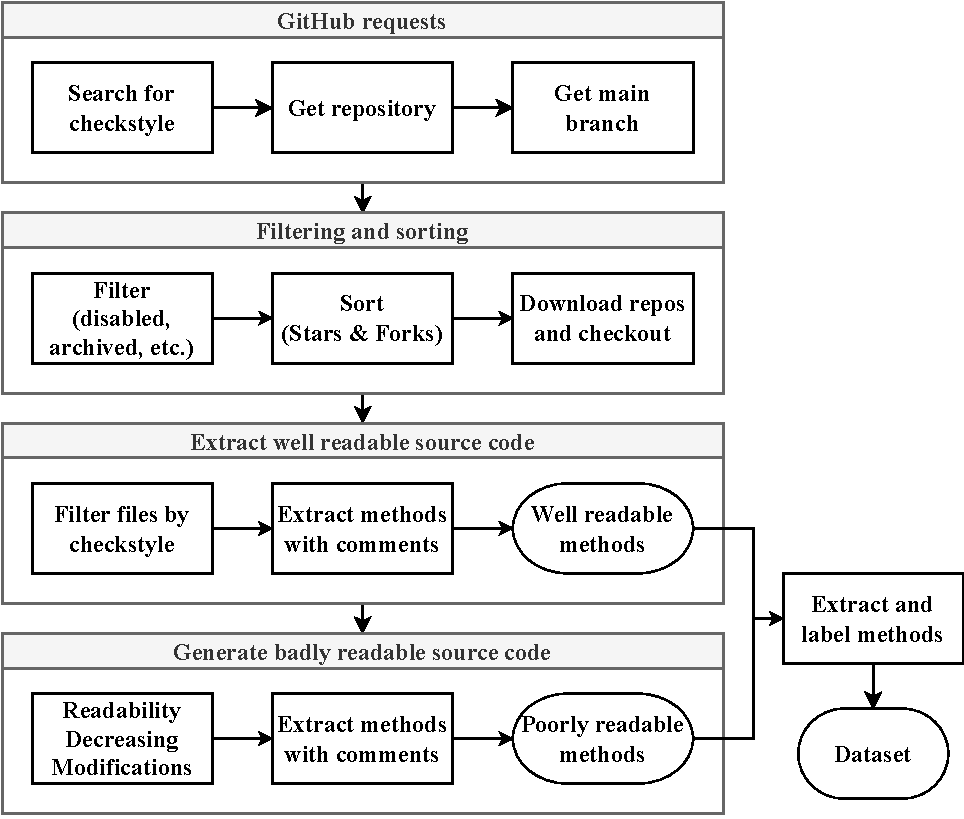
\includegraphics[width=0.9\textwidth]{img/dataset_generation.pdf}
		\caption{The used dataset generation approach.}
		\label{fig:dataset_generation}
	\end{figure}
	
	Our approach is divided into four parts (\autoref{fig:dataset_generation}). We use the first three steps to mine well readable Java code. In the final step, we modify the well readable code to achieve our second goal, namely poorly readable source code.
	
	We start by querying the GitHub REST API\curl{https://docs.github.com/en/rest}{2024-02-15} for repositories that use checkstyle (query string: \textquote{checkstyle filename:pom.xml}). The repository information (including the URL) is stored together with the main branches.
	We remove all repositories that are a fork of another repository, are archived, or are disabled.
	Additionally, we delete repositories whose language is not Java and those lacking a minimum of 20 stars and forks.
	% TODO: Intermediate result?
	% TODO: Why miteinbauen oder eher nicht?
	We sort the remaining repositories by their star and fork count (equally weighted). Then we clone the 100 best and check out their main branch.
	
	We run checkstyle against the project's own checkstyle configuration to obtain all Java class files that pass the own checkstyle test. For this we use a tool from Maximilian Jungwirth\curl{https://github.com/sphrilix/styler2.0}{2024-03-21} which is based on \textit{Styler}\curl{https://github.com/ASSERT-KTH/styler}{2024-03-11}~\cite{loriot2022styler}.
	From the Java class files that passed checkstyle, we extract all methods that have a comment of any kind at the beginning of the method. This results in \numOriginal methods which we assume to be well readable.
	
	We generate poorly readable code from the well readable one. To do this, we use the proposed \rdh tool (\Cref{REDEC}). We extract all methods starting with a comment.
	Originally, we planned not to require comments for the poorly readable dataset part. However, in this case, all well readable methods have a comment, while most of the poorly readable do not have one. This leads to shortcut learning, whether a method has a comment or not, instead of learning to distinguish the methods by all other criteria as well.
	
	We take the mined well readable methods and the modified poorly readable methods and combine them into the mined-and-modified dataset. We remove code snippets that are identical for the original and the modified variant (\Cref{REDEC}). We balance the dataset using random sampling.
	We label each well readable method and each poorly readable method with the corresponding mean rating scores obtained through a later user study (\Cref{Prolific Survey}).
	The created mined-and-modified dataset consists of \numSamplesAccurate code snippets.
	
\section{REDEC: Readability Decreaser} \label{REDEC}
	In this section, we take a look at how we achieved to decrease the readability of code using the \RDHa.
	\rdh uses a set of code modification heuristics that are applied to Java files. We call these \RDMs.
	
		\begin{table}[p]
		\centering
		\caption{All \RDMs with explanation and example.}
		\label{tab:rdh-description}
		\begin{tabular}{|p{0.03\textwidth}|p{0.24\textwidth}|p{0.43\textwidth}|p{0.135\textwidth}|}
			\hline
			\textbf{\#} & \textbf{Modification} & \textbf{Description} & \textbf{Example} \\
			\hline
			1 & \texttt{newline} & Replace a newline with none or multiple ones & \autoref{lst:java-method-poor}, Lines 5-6 \\
			\hline
			2 & \texttt{incTab} & Replace a tab indentation with none or multiple ones & \autoref{lst:java-method-poor}, Line 5 \\
			\hline
			3 & \texttt{decTab} & Replace a tab outdentation with none or more ones & \autoref{lst:java-method-poor}, Line 7 \\
			\hline
			4 & \texttt{space} & Replace a single space with multiple ones & \autoref{lst:java-method-poor}, Line 1 \\
			\hline
			5 & \texttt{newLine InsteadOf Space} & Replace a space with a newline & \autoref{lst:java-method-poor}, Line 3-4 \\
			\hline
			6 & \texttt{spaceInsteadOf Newline} & Replace a newline with a space & \autoref{lst:java-method-poor}, Line 2 \\
			\hline
			7 & \texttt{incTabInsteadOf DecTab} & Replace a tab outdentation with a tab indentation & \autoref{lst:java-method-poor}, Line 9 \\
			\hline
			8 & \texttt{decTabInsteadOf IncTab} & Replace a tab indentation with a tab outdentation & \autoref{lst:java-method-poor}, Line 8 \\
			\hline
			9 & \texttt{renameVariable} & Rename a variable declaration and its usages & \autoref{lst:java-method-poor}, Line 1-3 \\
			\hline
			10 & \texttt{renameField} & Rename a field declaration and its usages & \autoref{lst:java-class-file-poor}, Line 4 \\
			\hline
			11 & \texttt{renameMethod} & Rename a method declaration and its usages & \autoref{lst:java-method-poor}, Line 1 \\
			\hline
			12 & \texttt{inlineMethod} & Replace a method call with the called code & \autoref{lst:java-class-file-poor}, Line 7-8 \\
			\hline
			13 & \texttt{removeComment} & Remove a comment & \autoref{lst:java-method-poor}, Line 1 \\
			\hline
			14 & \texttt{add0} & Add a zero to a number & \autoref{lst:java-method-poor}, Line 2 \\
			\hline
			15 & \texttt{insertBraces} & Insert superfluous braces & \autoref{lst:java-method-poor}, Lines 3-4 \\
			\hline
			16 & \texttt{starImport} & Replace a specific imports with a star-import & \autoref{lst:java-class-file-poor}, Line 1 \\
			\hline
			17 & \texttt{inlineField} & Replace a static field with its value & \autoref{lst:java-class-file-poor}, Line 7 \\
			\hline
			18 & \texttt{partially Evaluate} & Partially evaluate a constant & \autoref{lst:java-class-file-poor}, Line 4 \\
			\hline
		\end{tabular}
	\end{table}
	
	\begin{listing}[p]
		\begin{sublisting}{\linewidth}
			\begin{minted}[linenos, frame=lines, framesep=2mm]{Java}
				/**
				* This method determines the sign of a given number and prints a corresponding message.
				*
				* @param number The input number to be checked.
				*/
				public static void checkNumberSign(int number) {
					if (number > 0) {
						System.out.println("Number is positive");
					} else if (number < 0) {
						System.out.println("Number is negative");
					} else {
						System.out.println("Number is zero");
					}
				}
			\end{minted}
			\caption{An example of a simple and well readable Java method.}
			\label{lst:java-method-well}
		\end{sublisting}
		
		\begin{sublisting}{\linewidth}
			\begin{minted}[linenos, frame=lines, framesep=2mm]{Java}
				public static void m0(int  v0) {
					if (v0 > (0+0)) { System.out.println("Number is positive");
					} else if ((v0 <
					0)) {
						System.out.println("Number is negative");
						
					} else {
						System.out.println("Number is zero");
				} }
			\end{minted}
			\caption{The same example as in \autoref{lst:java-method-well} but modified for poorer readability.}
			\label{lst:java-method-poor}
		\end{sublisting}
		\caption{Well readable (\autoref{lst:java-method-well}) vs. poorly readable (\autoref{lst:java-method-poor}) Java methods.}
		\label{lst:java-method}
	\end{listing}
	
	\begin{listing}[p]
		\begin{sublisting}{\linewidth}
			\begin{minted}[linenos, frame=lines, framesep=2mm]{Java}
				import java.util.Random;
				
				public class TimeConverter {
					public static final int MINUTES_PER_HOUR = 60;
					public static final int HOURS_PER_DAY = 24;
					public static final int MINUTES_PER_DAY = MINUTES_PER_HOUR * HOURS_PER_DAY;
					public static final int SEED = 4242;
					
					public int getRandomDays(int max) {
						Random random = new Random(SEED);
						return random.nextInt(max);
					}
					
					public int randomDaysInMinutes() {
						int days = getRandomDays(10);
						return days * MINUTES_PER_DAY;
					}
				}
			\end{minted}
			\caption{An example of a simple and well readable Java class file.}
			\label{lst:java-class-file-well}
		\end{sublisting}
		
		\begin{sublisting}{\linewidth}
			\begin{minted}[linenos, frame=lines, framesep=2mm]{Java}
				import java.util.*;
				
				public class TimeConverter {
					public static final int f0 = 1440;
					
					public int randomDaysInMinutes() {
						Random random = new Random(4242);
						int days = random.nextInt(10);
						return days * f0;
					}
				}
			\end{minted}
			\caption{The same example as in \autoref{lst:java-class-file-well} but modified for poorer readability.}
			\label{lst:java-class-file-poor}
		\end{sublisting}
		\caption{Well readable (\autoref{lst:java-class-file-well}) vs. poorly readable (\autoref{lst:java-class-file-poor}) Java class files.}
		\label{lst:java-class-file}
	\end{listing}

	%	From now on, we will use the abbreviation \textit{\rdh} or \textit{\rdh tool} when referring to the entire program. If a specific manipulation or a configuration of the \rdh tool is meant, we will use \textit{[name] \rdh} or \textit{[name]} instead.
	
	\rdh initially converts the Java code of a well readable Java class file into an Abstract Syntax Tree (AST, \Cref{Abstract Syntax Tree}) using the spoon library\curl{https://spoon.gforge.inria.fr/}{2024-15-02}~\cite{pawlak2016spoon}. In the end \rdh parses the AST back to Java code using the Pretty Printer of the spoon library~\cite{pawlak2016spoon}. If nothing else is done, this results in \nonet. Note that the code of \nonet is slightly different from the original code, as the Pretty Printer overwrites the styling and formatting of the original code by its default formatting.
	
	%	Renaming is done while the code is in its AST representation to ensure that the declarations and usages of variables (\texttt{renameVariable}), fields (\texttt{renameField}) and methods (\texttt{renameMethod}) are all renamed to the same new identifier.
	
	% What is available
	Various modifications can be made between the two steps and during pretty-printing. You can find a description of each modification in \autoref{tab:rdh-description} and examples of the modifications in \autoref{lst:java-method} and \autoref{lst:java-class-file}.
	
	In \autoref{tab:rdh-description} tab \textit{indentation} refers to the process of adding a tab ($\backslash t$) while \textit{outdentation} refers to the opposite, namely removing a tab ($\backslash t$). 
	%	For example, if the current tab count is 1 ($\backslash t \langle CODE \rangle$) (\autoref{lst:example-method-well}, Line 7) a tab indentation results in a tab count of 2 ($\backslash t \backslash t \langle CODE \rangle $) (\autoref{lst:example-method-well}, Line 8) and then a tab outdentation results in a tab count of 1 again ($ \backslash t \langle CODE \rangle$) (\autoref{lst:example-method-well}, Line 9).
	For example:
	\begin{enumerate}
		\item The current tab count is 1 ($\backslash t \langle CODE \rangle$) (\autoref{lst:java-method-well} Line 7).
		\item In the next line, we perform a tab indentation.
		\item The current tab count is now 2 ($\backslash t \backslash t \langle CODE \rangle $) (\autoref{lst:java-method-well}, Line 8).
		\item In the next line, we perform a tab outdentation.
		\item The current tab count is now 1 ($\backslash t \langle CODE \rangle $) (\autoref{lst:java-method-well}, Line 9).
	\end{enumerate}
		
	\rdh performs one part of the modifications on the Abstract Syntax Tree (AST) representation of the Java files. It executes another part when pretty-printing the AST back into Java files. The first part is executed on the AST to ensure that the functionality stays the same. For example, when REDEC renames a method, the declaration along with all references are renamed.	
	The second part is not encoded in the AST and is therefore executed at the source code level after the reverse transformation. For example, the AST does not encode line breaks. Changes to these line breaks must be applied to the source code rather than the AST. You can see which modifications are applied when in \autoref{tab:rdh-characteristics}.
	
	\rdh applies a modification to each occurrence of the object it refers to with a specified probability. Due to the use of probabilities it can happen that no modification is applied. For example, we execute \rdh and set only \texttt{removeComment} to a probability of 10~\%. Then the tool removes each comment of the given Java class files with a probability of 10~\%. The exact amount of removed comments is uncertain. It can happen (especially for short methods within the class files) that a method is not changed at all. For example, if a method only has a single comment and we use \texttt{removeComment}, the probability that the method is not changed (besides the changes of \nonet) is 90~\%.

	
%	We perform certain modifications on the AST to ensure that the functionality stays the same.
%	We apply other modifications on source code during pretty-printing as they cannot be displayed in the AST.
%	In \autoref{tab:rdh-characteristics} we can see which modifications are applied when.
	
	\begin{table}[tb]
		\centering
		\caption{Available \RDMs along with their execution type (on AST or Code), their configuration type (an array of probabilities or a single one), and whether they are included in the final dataset. \Cref{appendix:rdh-config-file} for a concrete configuration example.}
		\label{tab:rdh-characteristics}
		\begin{tabular}{llllc}
			\toprule
			\# & \Mod 						 & AST/Code 	& Config. Type 	& In Dataset \\
			\midrule
			1  & \texttt{newline}                & Code			& Array 		& \checkmark \\
			2  & \texttt{incTab}                 & Code			& Array 		& \checkmark \\
			3  & \texttt{decTab}                 & Code			& Array 		& \checkmark \\
			4  & \texttt{space}                  & Code			& Array 		& \checkmark \\
			5  & \texttt{newLineInsteadOfSpace}  & Code			& Single 		& \checkmark \\
			6  & \texttt{spaceInsteadOfNewline}  & Code			& Single 		& \checkmark \\
			7  & \texttt{incTabInsteadOfDecTab}  & Code			& Single 		& \checkmark \\
			8  & \texttt{decTabInsteadOfIncTab}  & Code			& Single 		& \checkmark \\
			9  & \texttt{renameVariable}         & AST			& Single 		& \checkmark \\
			10 & \texttt{renameField}            & AST			& Single 		& \checkmark \\
			11 & \texttt{renameMethod}           & AST			& Single 		& \checkmark \\
			12 & \texttt{inlineMethod}           & AST			& Single		& \\
			13 & \texttt{removeComment}          & Code			& Single 		& \checkmark \\
			14 & \texttt{add0}                   & AST			& Single		& \\
			15 & \texttt{insertBraces}           & AST			& Single		& \\
			16 & \texttt{starImport}             & AST			& Single		& \\
			17 & \texttt{inlineField}            & AST			& Single		& \\
			18 & \texttt{partiallyEvaluate}      & AST			& Single		& \\
			\bottomrule
		\end{tabular}
	\end{table}
	
%	\begin{itemize}
%		\item \texttt{renameVariable}: Renaming a variable declaration and its usages (\autoref{lst:example-method-badly}, Line 1)
%		\item \texttt{renameField}: Renaming a field declaration and its usages (\autoref{lst:java-class-file-rdh}, Line 6)
%		\item \texttt{renameMethod}: Renaming a method declaration and its usages (\autoref{lst:example-method-badly}, Line 1)
%		\item \texttt{add0}: Adding zero to numbers (\autoref{lst:example-method-badly}, Line 3)
%		\item \texttt{insertBraces}: Inserting superfluous braces (\autoref{lst:example-method-badly}, Line 1)
%		\item \texttt{starImport}: Replacing specific imports with star-import (\autoref{lst:java-class-file-rdh}, Line 1)
%		\item \texttt{inlineField}: Inlining the values of static fields into the code (\autoref{lst:java-class-file-rdh}, Line 8)
%		\item \texttt{partiallyEvaluate}: Partially evaluate constants (\autoref{lst:java-class-file-rdh}, Line 6)
%	\end{itemize}
	
%	\begin{table}[tb]
%		\centering
%		\caption{The \RDMs that are performed on the AST.}
%		\vspace{8pt}
%		\label{tab:ast-\RDMs}
%		\begin{tabular}{|p{0.15\textwidth}|p{0.6\textwidth}|p{0.125\textwidth}|}
%			\hline
%			\textbf{\rdh} & \textbf{Description} & \textbf{Example} \\
%			\hline
%			\texttt{rename Variable} & Renaming a variable declaration and its usages & \autoref{lst:example-method-badly}, Line 1 \\
%			\hline
%			\texttt{rename Field} & Renaming a field declaration and its usages & \autoref{lst:java-class-file-rdh}, Line 6 \\
%			\hline
%			\texttt{rename Method} & Renaming a method declaration and its usages & \autoref{lst:example-method-badly}, Line 1 \\
%			\hline
%			\texttt{add0} & Adding zero to numbers & \autoref{lst:example-method-badly}, Line 3 \\
%			\hline
%			\texttt{insert Braces} & Inserting superfluous braces & \autoref{lst:example-method-badly}, Line 1 \\
%			\hline
%			\texttt{star Import} & Replacing specific imports with star-import & \autoref{lst:java-class-file-rdh}, Line 1 \\
%			\hline
%			\texttt{inline Field} & Inlining the values of static fields into the code & \autoref{lst:java-class-file-rdh}, Line 8 \\
%			\hline
%			\texttt{partially Evaluate} & Partially evaluate constants & \autoref{lst:java-class-file-rdh}, Line 6 \\
%			\hline
%		\end{tabular}
%	\end{table}
		
	By default, \rdh generates the new identifiers for the rename modifications (\texttt{renameVariable}, \texttt{renameField}, and \texttt{renameMethod}) in an iterating manner. For each class file, we start with \textit{v0} for variables, \textit{f0} for fields, and \textit{m0}. We increase the index of each (0 at the beginning) by 1 whenever a name is used.
	We also added a mode that uses Code2Vec~\cite{alon2019code2vec} for the generation of identifiers for \texttt{renameMethod} instead. With that, we can predict more realistic method names. Code2Vec generates multiple method name predictions at once. By picking not the best one but instead the one with the longest name we aim to decrease readability while choosing realistic method names.
		
%	\begin{center}
%		\begin{tabularx}{\textwidth}{|X|X|X|}
%			\hline
%			\textbf{\rdh} & \textbf{Description} & \textbf{Example} \\
%			\hline
%			\texttt{newline} & Replacing newlines with none or multiple ones & \autoref{lst:java-class-file-rdh}, Line 2-6 \\
%			\hline
%			\texttt{incTab} & Replace a tab indentation with none or multiple ones & \autoref{lst:example-method-badly}, Line 1 \\
%			\hline
%			\texttt{decTab} & Replace a tab outdentation with one or more ones & \autoref{lst:example-method-badly}, Line TODO \\
%			\hline
%			\texttt{space} & Replacing a single space with multiple ones & \autoref{lst:example-method-badly}, Line 1 \\
%			\hline
%			\texttt{newLine InsteadOf Space} & Replacing a space with a newline & \autoref{lst:example-method-badly}, Line TODO \\
%			\hline
%			\texttt{space InsteadOf Newline} & Replacing a newline with a space & \autoref{lst:example-method-badly}, Line 1 \\
%			\hline
%			\texttt{incTab InsteadOf DecTab} & Replace a tab outdentation with an indentation & \autoref{lst:example-method-badly}, Line 2 \\
%			\hline
%			\texttt{decTab InsteadOf IncTab} & Replace a tab indentation with an outdentation & \autoref{lst:example-method-badly}, Line 2 \\
%			\hline
%		\end{tabularx}
%	\end{center}
	
	
%	table}[tb]
%		\centering
%		\caption{The \RDMs that are performed while pretty-printing}
%		\vspace{8pt}
%		\label{tab:code-\RDMs}
%		\begin{tabular}{|p{0.15\textwidth}|p{0.6\textwidth}|p{0.125\textwidth}|}
%			\hline
%			\textbf{\rdh} & \textbf{Description} & \textbf{Example} \\
%			\hline
%			\texttt{newline} & Replacing newlines with none or multiple ones & \autoref{lst:java-class-file-rdh}, Line 2-6 \\
%			\hline
%			\texttt{incTab} & Replace a tab indentation with none or multiple ones & \autoref{lst:example-method-badly}, Line 1 \\
%			\hline
%			\texttt{decTab} & Replace a tab outdentation with one or more ones & \autoref{lst:example-method-badly}, Line TODO \\
%			\hline
%			\texttt{space} & Replacing a single space with multiple ones & \autoref{lst:example-method-badly}, Line 1 \\
%			\hline
%			\texttt{newLine InsteadOf Space} & Replacing a space with a newline & \autoref{lst:example-method-badly}, Line TODO \\
%			\hline
%			\texttt{space InsteadOf Newline} & Replacing a newline with a space & \autoref{lst:example-method-badly}, Line 1 \\
%			\hline
%			\texttt{incTab InsteadOf DecTab} & Replace a tab outdentation with an indentation & \autoref{lst:example-method-badly}, Line 2 \\
%			\hline
%			\texttt{decTab InsteadOf IncTab} & Replace a tab indentation with an outdentation & \autoref{lst:example-method-badly}, Line 2 \\
%			\hline
%		\end{tabular}
%	\end{table}

	
%	\begin{itemize}
%		\item \texttt{newline}: Replacing newlines with none or multiple ones (\autoref{lst:java-class-file-rdh}, Line 2-6)
%		\item \texttt{incTab}: Replace a tab indentation more with none or multiple ones (\autoref{lst:example-method-badly}, Line 1)
%		\item \texttt{decTab}: Replace a tab outdentation with one or more ones (\autoref{lst:example-method-badly}, Line TODO)
%		\item \texttt{space}: Replacing a single space with multiple ones (\autoref{lst:example-method-badly}, Line 1)
%		\item \texttt{newLineInsteadOfSpace}: Replacing a space with a newline (\autoref{lst:example-method-badly}, Line TODO)
%		\item \texttt{spaceInsteadOfNewline}: Replacing a newline with a space (\autoref{lst:example-method-badly}, Line 1)
%		\item \texttt{incTabInsteadOfDecTab}: Replace a tab outdentation with a indentation (\autoref{lst:example-method-badly}, Line 2)
%		\item \texttt{decTabInsteadOfIncTab}: Replace a tab indentation with a outdentation (\autoref{lst:example-method-badly}, Line 2)
%	\end{itemize}
	\rdh does not support the removal of spaces, as this can cause keywords and/or identifiers to merge, which can result in the code no longer compiling.
	For example, consider the space between \textit{int} and \textit{number} in Line 6 in \Cref{lst:example-method}. If we remove the space, the result is \textit{intnumber}. Since the syntax is violated, the code no longer compiles.
	
%	\begin{sloppypar}
%	These include adding spaces (\texttt{space}), replacing spaces with newlines (\texttt{spaceInsteadOfNewline}), adding or removing newlines (\texttt{newline}), replacing newlines with spaces (\texttt{newLineInsteadOfSpace}), and changing the indentation of code in term of tabs (\texttt{incTab}, \texttt{decTab}, \texttt{incTabInsteadOfDecTab}, \texttt{decTabInsteadOfIncTab}).
%	\end{sloppypar}

	% What did we exclude and why
	For the final dataset, we exclude some of the modifications as we can see in \autoref{tab:rdh-characteristics}.
	We exclude \texttt{inlineMethod} as it increased the length of methods drastically and made the methods too long.
	While \texttt{starImport} might have an impact on the readability of class files, it has none on methods, since in Java the import statements are not within the methods. As we finally extract methods for our dataset, \texttt{starImport} has no impact.
	%	We did not include \texttt{partiallyEvaluate} as it might be that this modification increases readability instead of decreasing it.
	We chose not to include \texttt{add0}, \texttt{insertBraces}, \texttt{inlineField}, and \texttt{partiallyEvaluate} for the reason of a limited survey capacity.
	For the same reason, we do not investigate the usage of Code2Vec for \texttt{renameMethod} either.

	%	\begin{figure}[tb]
	%		\centering
	%		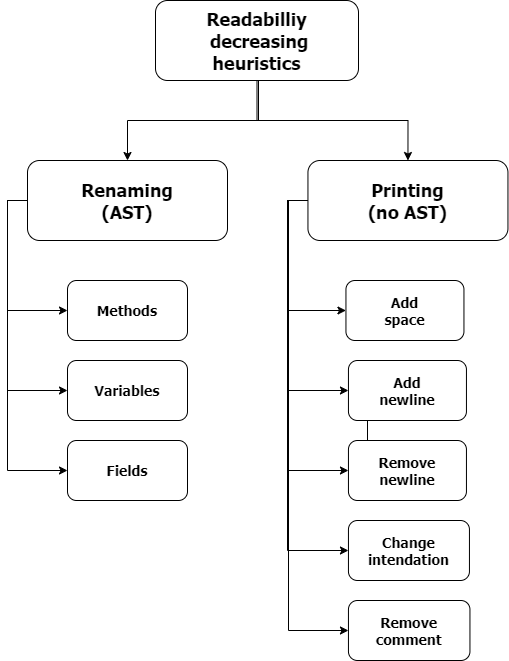
\includegraphics[width=0.75\textwidth]{img/\rdh.png}
	%		\caption{The available \RDHa.}
	%		\label{fig:rdh}
	%	\end{figure}
	
	% Cofig: Array vs Single
	The \rdh tool works with a configuration file in which one can specify a probability for each available \mod.
	For \mods of configuration type \textit{Array} (\texttt{newline}, \texttt{incTab}, \texttt{decTab} and \texttt{space}), an array of probabilities must be defined for the respective number of replacements. The probabilities of the array must sum up to 1.
	For \mods of configuration type \textit{Single} a single probability must be defined (\autoref{tab:rdh-characteristics}).
	For example, \texttt{spaceInsteadOfNewline} can be configured with $0.05$ meaning that each space is replaced with a newline ($\backslash n$) with a probability of 5~\%.
	\texttt{space} can be configured with $[0.0, 0.7, 0.2, 0.1]$ meaning that each space is replaced with
	\begin{itemize}
		\item no space with a probability of 0~\%
		\item a single space with a probability of 70~\% (no change)
		\item two spaces with a probability of 20~\%
		\item three spaces with a probability of 10~\% 
	\end{itemize}
		
	% Config: 
	We select the probabilities for the generated code snippets so that they are still realistic, i.e. that they could be written by humans. This is done empirically by examining exemplary outputs of REDEC with different configurations. You can find the resulting configurations in \autoref{tab:rdh_configurations} and an exemplary file for \nonet in \Cref{appendix:rdh-config-file}.
	\texttt{all7} is the average of the other 7 configurations: The probabilities of the other 7 configurations are added to one configuration and each probability is divided by 7.
	There is a special case regarding \texttt{removeComment}: \texttt{comments-remove} and \texttt{all7} use \texttt{removeComment} at 100~\% for the user survey (\Cref{Survey}). The reason for this is that a method without comments is realistic. For training and evaluation of the deep-learning model, the probability was set to 10~\% (for both affected configurations, \texttt{all7} and \texttt{removeComment}) to avoid shortcut learning (\Cref{Model training results}).
	
	%	\begin{table}[tb]
		%		\centering
		%		\caption{Chosen configurations and their probabilities for the \RDMs.}
		%		\vspace{8pt}
		%		\label{tab:rdh_configurations}
		%		\begin{tabular}{|l|l|l|}
			%			\hline
			%			\textbf{Configuration} & \textbf{Probabilities} \\
			%			\hline
			%			none & - \\
			%			\hline
			%			comments-remove & removeComment: 0.1 \\
			%			\hline
			%			newline-instead-of-space & newLineInsteadOfSpace: 0.15 \\
			%			\hline
			%			newlines-few & \begin{tabular}[t]{@{}l@{}}removeNewline: 0.3 \\ spaceInsteadOfNewline: 0.05\end{tabular} \\
			%			\hline
			%			newlines-many & \begin{tabular}[t]{@{}l@{}}add1Newline: 0.15 \\ add2Newlines: 0.05\end{tabular} \\
			%			\hline
			%			rename & \begin{tabular}[t]{@{}l@{}}renameVariable: 0.3 \\ renameField: 0.3 \\ renameMethod: 0.3\end{tabular} \\
			%			\hline
			%			spaces-many & \begin{tabular}[t]{@{}l@{}}Add1Space: 0.2 \\ Add2Spaces: 0.1 \\ spaceInsteadOfNewline: 0.05\end{tabular} \\
			%			\hline
			%			tabs & \begin{tabular}[t]{@{}l@{}}remove1IncTab: 0.2 \\ add1IncTab: 0.1 \\ remove1DecTab: 0.1 \\ add1DecTab: 0.1 \\ incTabInsteadOfDecTab: 0.05 \\ decTabInsteadOfIncTab: 0.05\end{tabular} \\
			%			\hline
			%			all7 & all probabilites/7\\
			%			\hline
			%		\end{tabular}
		%
		%	\end{table}
	
	\begin{table}[tb]
		\centering
		\caption{Chosen configurations and their probabilities for the \RDMs. For better readability, we write \textit{addX} and \textit{removeX} instead of the array configurations. For example, we write \textit{Add1Space:~20~\%} and \textit{Add2Spaces:~10~\%}, but the configuration is \textit{space:~[0.0, 0.7, 0.2, 0.1]}.}
		\label{tab:rdh_configurations}
		\begin{tabular}{|l|l|l|}
			\hline
			\textbf{Configuration} & \textbf{Probabilities} \\
			\hline
			just-pretty-print & - \\
			\hline
			comments-remove & removeComment: 10 \% or 100 \%  \\
			\hline
			newline-instead-of-space & newLineInsteadOfSpace: 15 \% \\
			\hline
			newlines-few & \begin{tabular}[t]{@{}l@{}}removeNewline: 30 \% \\ spaceInsteadOfNewline: 5 \%\end{tabular} \\
			\hline
			newlines-many & \begin{tabular}[t]{@{}l@{}}add1Newline: 15 \% \\ add2Newlines: 5 \%\end{tabular} \\
			\hline
			rename & \begin{tabular}[t]{@{}l@{}}renameVariable: 30 \% \\ renameField: 30 \% \\ renameMethod: 30 \%\end{tabular} \\
			\hline
			spaces-many & \begin{tabular}[t]{@{}l@{}}Add1Space: 20 \% \\ Add2Spaces: 10 \% \\ spaceInsteadOfNewline: 5 \%\end{tabular} \\
			\hline
			tabs & \begin{tabular}[t]{@{}l@{}}remove1IncTab: 20 \% \\ add1IncTab: 10 \% \\ remove1DecTab: 10 \% \\ add1DecTab: 10 \% \\ incTabInsteadOfDecTab: 5 \% \\ decTabInsteadOfIncTab: 5 \%\end{tabular} \\
			\hline
			all7 & all probabilites/7\\
			\hline
		\end{tabular}
	\end{table}
	
	%	\begin{table}[h]
		%		\centering
		%		\caption{Chosen configurations and their probabilities for the \RDMs}
		%		\vspace{8pt}
		%		\label{tab:rdh_configurations}
		%		\begin{tabular}{ll}
			%			\toprule
			%			\textbf{Configuration} & \textbf{Probabilities} \\
			%			\midrule
			%			none & - \\
			%			comments-remove & removeComment: 1.0 \\
			%			newline-instead-of-space & newLineInsteadOfSpace: 0.15 \\
			%			newlines-few & \begin{tabular}[t]{@{}l@{}}removeNewline: 0.3 \\ spaceInsteadOfNewline: 0.05\end{tabular} \\
			%			newlines-many & \begin{tabular}[t]{@{}l@{}}add1Newline: 0.15 \\ add2Newlines: 0.05\end{tabular} \\
			%			rename & \begin{tabular}[t]{@{}l@{}}renameVariable: 0.3 \\ renameField: 0.3 \\ renameMethod: 0.3\end{tabular} \\
			%			spaces-many & \begin{tabular}[t]{@{}l@{}}Add1Space: 0.2 \\ Add2Spaces: 0.1 \\ spaceInsteadOfNewline: 0.05\end{tabular} \\
			%			tabs & \begin{tabular}[t]{@{}l@{}}remove1IncTab: 0.2 \\ add1IncTab: 0.1 \\ remove1DecTab: 0.1 \\ add1DecTab: 0.1 \\ incTabInsteadOfDecTab: 0.05 \\ decTabInsteadOfIncTab: 0.05\end{tabular} \\
			%			all7 & all probabilities/7 \\
			%			\bottomrule
			%		\end{tabular}
		%	\end{table}
	
	% Config Examples

	
%	Some of the heuristics were not included in the final version of the mined-and-modified dataset. You can find them in \autoref{tab:not-included-\RDMs} together with the reason why they were not included.
%	\begin{table}[tb]
%		\centering
%		\caption{\RDMs that are not included in the final version of the mined-and-modified dataset and why.}
%		\vspace{8pt}
%		\label{tab:not-included-\RDMs}
%		\begin{tabular}{ll}
%			\toprule
%			Heuristic & Reason \\
%			\midrule
%			\texttt{inlineMethod} & Makes methods too long \\
%			\texttt{add0} & Limited survey capacity \\
%			\texttt{insertBraces} & Limited survey capacity \\
%			\texttt{starImport} & No effect after comment extraction \\
%			\texttt{inlineField} & Limited survey capacity \\
%			\texttt{partiallyEvaluate} & Might increase readability \\
%			\bottomrule
%		\end{tabular}
%	\end{table}

%	\begin{table}[tb]
%		\centering
%		\caption{Available \RDMs. For heuristics $1-4$ (\texttt{newline}, \texttt{incTab}, \texttt{decTab} and \texttt{space}), several probabilities can be defined for the respective number of replacements (\Cref{appendix:rdh-config-file}).}
%		\vspace{8pt}
%		\label{tab:\RDMs}
%		\begin{tabular}{lllc}
%			\toprule
%			\# & Heuristic 						 & On AST/Code & n Final Dataset \\
%			\midrule
%			1  & \texttt{newline}                & Code			& \checkmark \\
%			2  & \texttt{incTab}                 & Code			& \checkmark \\
%			3  & \texttt{decTab}                 & Code			& \checkmark \\
%			4  & \texttt{space}                  & Code			& \checkmark \\
%			5  & \texttt{newLineInsteadOfSpace}  & Code			& \checkmark \\
%			6  & \texttt{spaceInsteadOfNewline}  & Code			& \checkmark \\
%			7  & \texttt{incTabInsteadOfDecTab}  & Code			& \checkmark \\
%			8  & \texttt{decTabInsteadOfIncTab}  & Code			& \checkmark \\
%			9  & \texttt{renameVariable}         & AST			& \checkmark \\
%			10 & \texttt{renameField}            & AST			& \checkmark \\
%			11 & \texttt{renameMethod}           & AST			& \checkmark \\
%			12 & \texttt{inlineMethod}           & AST			& \\
%			13 & \texttt{removeComment}          & Code			& \checkmark \\
%			14 & \texttt{add0}                   & AST			& \\
%			15 & \texttt{insertBraces}           & AST			& \\
%			16 & \texttt{starImport}             & AST			& \\
%			17 & \texttt{inlineField}            & AST			& \\
%			18 & \texttt{partiallyEvaluate}      & AST			& \\
%			\bottomrule
%		\end{tabular}
%	\end{table}
	
	% Method extraction
	After applying \rdh to the Java files, we extract the methods. We require a method comment for all methods (\Cref{Dataset Generation Approach}). We therefore use \texttt{removeComment} after completing the method extraction.
	
\section{Construction of Questionnaires} \label{Construction of Questionnaires}
	We evaluate the generated dataset and the new approach with a survey (\Cref{Survey}). However, we cannot evaluate all mined-and-modified methods as the original methods consist of \numOriginal samples and there is an infinite number of possible configurations for \rdh that can be applied to each method.
	Therefore, we apply stratified sampling (\Cref{Stratified Sampling})~\cite{thompson2012sampling}, create specific configurations, and select the methods for our survey based on the resulting strata. You can find an overview of the approach in \autoref{fig:survey_pipeline}.
	
	\begin{figure}[tb]
		\centering
		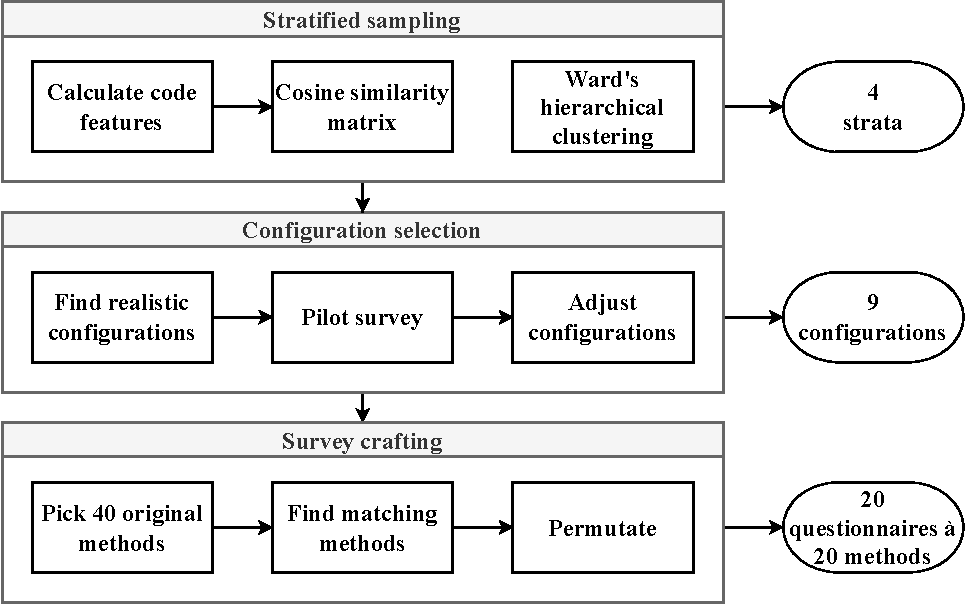
\includegraphics[width=0.9\textwidth]{img/survey_pipeline.pdf}
		\caption{Steps performed to craft questionnaires from the mined-and-modified dataset.}
		\label{fig:survey_pipeline}
	\end{figure}
	
	\textbf{Stratified sampling:} 
	We want to categorize the Java methods to make it easier to decide which ones to select. We also want to avoid over-representing very simple methods, such as Getters and Setters. Therefore, our first step is to apply stratified sampling~\cite{thompson2012sampling}. This allows us to divide the methods into different groups, so-called strata, based on handcrafted features (\Cref{Conventional Calculation Approaches}).
	Since we want to compare the original methods with their modified variants later, we perform the sampling only for the original methods and add the \rdh methods in a later step.

	We first calculate the handcrafted features for the original code snippets. We therefore use a tool of \citeauthor{scalabrino2018comprehensive}~\cite{scalabrino2018comprehensive}. We calculate a 110-dimensional feature vector for each original code snippet.
	Such features are, for example, the average line length and the code snippet length.
	Next, we compute the cosine similarity matrix between all feature vectors using scikit\curl{https://scikit-learn.org/stable/modules/generated/sklearn.metrics.pairwise.cosine_similarity.html}{2024-02-20}.
	The matrix contains the similarity between all calculated vector pairs, based on the cosine of the angle between the vectors. The distance between multiple vectors is called the cosine distance.
	Finally, using the fastcluster implementation~\cite{mullner2013fastcluster} of Ward's hierarchical clustering we cluster the methods into an arbitrary amount of strata.
	
	In each clustering step $x$, the two strata with the smallest cosine distance between their feature vectors are merged into one. This distance is the merged distance of the step, $MD_x$.
	For further investigation, we also calculate the difference between the merge distance and the merged distance of the previous step $x-1$:
	\begin{center}
		$\text{Difference to previous} = MD_x - MD_{x-1}$
	\end{center}
	For each step, you can find the merge distance together with the difference to the previous step in \autoref{fig:strata_merge_distances}.
	
	The graph shows that a strata size of 4 makes the most sense: the merge distance of 5 to 4 is small, so we should still perform this merge, but the merge distance of 4 to 3 is large, so it is better not to perform this merge.
	In general, other layer sizes are also suitable where the merge distance to the respective step is small and to the next step is large. The \textit{difference to previous} graph (\autoref{fig:strata_merge_distances}) depicts those points as minima. Therefore, for example, 6 or 8 are also suitable.
	Of these suitable sizes, a strata size of 4 is the last option with a small merge distance before the number of strata becomes too small.
	We therefore opted for 4 strata.
	
	We identify the type of methods within each of the 4 strata as described in \autoref{tab:strata_info}. We also add the number of methods within each stratum. 
	Stratum 0 comprises simple methods, such as Getters and Setters. Stratum 1 consists of the most complex methods across all strata. 
	Stratum 2 is characterized by methods containing numeric values with unexplained meanings, commonly referred to as magic numbers. Compared to the other strata, Stratum 2 has a smaller scope of 78 methods. 
	Stratum 3 contains methods of medium complexity that exceed the simplicity of the Getters and Setters in Stratum 0, but do not come close to the complexity of the methods in Stratum 1. 
	Overall, we split the methods according to their complexity, ranging from simple (Stratum 0) to medium (Stratum 3) to complex (Stratum 1), while Stratum 2 is a by-product.
	
	\begin{figure}[tb]
		\centering
		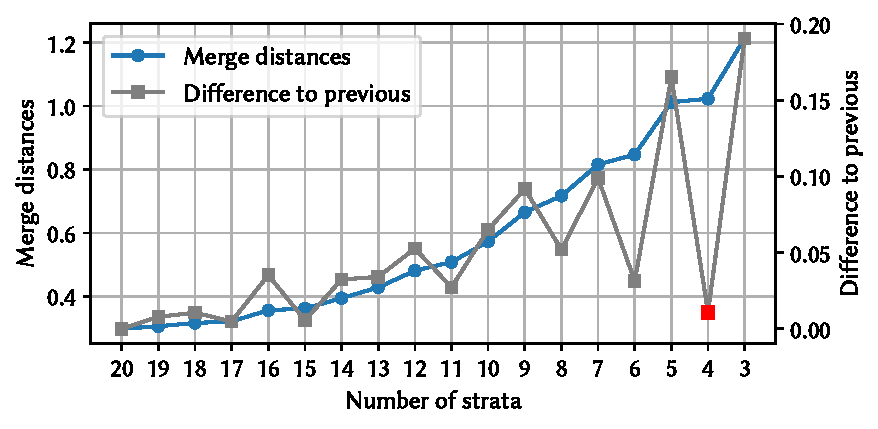
\includegraphics[width=\textwidth]{img/strata_merge_distances.pdf}
		\caption{Merge distances and difference to previous merge distance. The optimal difference to the previous merge distance is highlighted in red.} 
		\label{fig:strata_merge_distances}
	\end{figure}
	
	\textbf{Configuration selection:} The next step is to find realistic configurations for the \rdh tool. We select the first configurations by manually checking individual outputs of \rdh. Then we conduct a pilot study and adjust the configurations based on the feedback.
	The final 9 configurations can be found in \autoref{tab:rdh_configurations}. Together with the original methods this results in 10 groups.
	
%	\begin{table}[tb]
%		\centering
%		\caption{Computed strata and manually assigned name based on the methods within.}
%		\vspace{8pt}
%		\label{tab:survey_strata_labeles}
%		\begin{tabular}{ll}
%			\toprule
%			Stratum & Method Type \\
%			\midrule
%			Stratum 0 & Simple methods \\
%			Stratum 1 & Complex methods \\
%			Stratum 2 & Magic number methods \\
%			Stratum 3 & Medium complex methods \\
%			\bottomrule
%		\end{tabular}
%	\end{table}
		

	
%	\begin{table}[tb]
%		\centering
%		\caption{Strata distribution of sampled methods.}
%		\vspace{8pt}
%		\label{tab:sampled_methods}
%		\begin{tabular}{lrr}
%			\toprule
%			Stratum & Percentage & Count \\
%			\midrule
%			Stratum 0 & 10 \% & 4 \\
%			Stratum 1 & 40 \% & 16 \\
%			Stratum 2 & 10 \% & 4 \\
%			Stratum 3 & 40 \% & 16 \\
%			\midrule
%			\textbf{Total} & \textbf{100 \%} & \textbf{40} \\
%			\bottomrule
%		\end{tabular}
%
%	\end{table}
	
	\begin{table}[tb]
		\centering
		\caption{The strata properties (name, manually assigned type of methods, and the method count) and the number of methods sampled for the survey (in percent and the total count).}
		\label{tab:strata_info}
		\begin{tabular}{llr|rr}
			\toprule
			\multicolumn{3}{l|}{\textbf{Properties}} & \multicolumn{2}{l}{\textbf{Sampling}} \\
			Name & Type of Methods & Count & Percentage & Count \\
			\midrule
			Stratum 0 & Simple methods & 19016 & 10~\% & 4 \\
			Stratum 1 & Complex methods & 4280 & 40~\% & 16 \\
			Stratum 2 & Magic number methods & 78 & 10~\% & 4 \\
			Stratum 3 & Medium complex methods & 15938 & 40~\% & 16 \\
			\midrule
			\textbf{Total} & & \textbf{\numOriginal} & \textbf{100~\%} & \textbf{40} \\
			\bottomrule
		\end{tabular}
	\end{table}
	
	\textbf{Survey crafting:} Finally, we craft the questionnaires from the strata. We decided to provide all 10 configurations for each original method as we want to compare the original methods with their \rdh variants. We have a survey capacity of 400 code snippets (\Cref{Prolific Survey}). Therefore, the capacity for each \rdh variant is $400/10 = 40$ code snippets. We start by selecting 40 original code snippets and then we add all their \rdh variants.
	We opt for a random sample within the strata. However, we distribute the 40 snippets across the strata as shown in \Cref{tab:strata_info}:
	We sample 4 methods each from Stratum~0 and Stratum~2 and 16 methods each from Stratum~1 and Stratum~3.
	The reason for choosing this approach is the relatively high frequency of methods that do not differ from their original methods in Stratum 0 and Stratum 2 (\autoref{fig:sampling_not_different_overall}). Additionally, simple methods are rather uninteresting for the classification of readability, as they can be generated (e.g. by IDEs) and usually follow a straightforward pattern.
	
	%TODO: Add and link drawio "questionaire" graph
	\begin{figure}[tb]
		\centering
		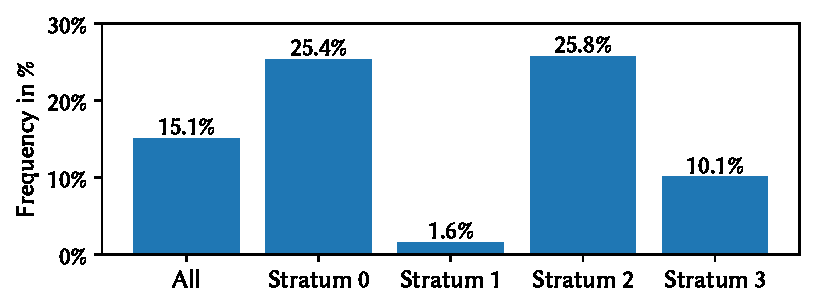
\includegraphics[width=\textwidth]{img/sampling_not_different_overall_ylim.pdf}
		\caption{Frequency of the case that a \rdh variant is not different from its original method.} 
		\label{fig:sampling_not_different_overall}
	\end{figure}
		
	After selecting the 40 original methods, we select all $9*40$ (\#configurations $*$ \#variant-capacity) \rdh variants that belong to the original methods next. We do this automatically based on the names of the original methods and the names of the \rdh variant methods. If \rdh renamed the method at an earlier stage due to the method renaming \mod, the new method no longer matches the original method, in which case we match them manually.
		
	Once we collected all 400 methods, we distributed them across the 20 questionnaires, each with 20 methods. To not manipulate the raters, we decided that a variant of each method must only appear once in each questionnaire. For example, if the original method is in one questionnaire, the \texttt{removeComment} variant (or another variant of the same method) must not be included in the same questionnaire.
		
	For this purpose, we create four permutation matrices with 10 snippets each. We chose the number 10 because it is possible to distribute 10 snippets, each with 10 variants, across at least 10 survey questionnaires without violating our condition. By combining two 10-permutation matrices, we achieve to create 10 survey questionnaires with 20 code snippets each. This approach implies that each questionnaire contains each kind of variant exactly twice. By doing this twice, we obtain the desired distribution of 20 questionnaires with 20 methods each. Our condition applies: There is only one variant of the same method in each questionnaire.
		
	Finally, the methods of each questionnaire are randomly shuffled within itself. We do this to minimize the impact of the position of a snippet or variant within a survey on the rating.

%	Each snippet of the well readable code (original) is labeled with the mean value of all ratings of the original variant across all survey results. Similarly, we label the all7 code snippets with their mean value. Note that in the binary classification with the underlying Towards model, this results in the original methods being labeled well readable and the all7 \rdh poorly readable.	
	
%	% We conclude a user study to evaluate the newly generated data for readability classifier models.
%	The goal of the user study is to answer the following key questions:
%	
%	\begin{enumerate}
%		\item Does the well-readable-assumption (\Cref{well-readable-assumption}) hold?
%		\item Does the poorly-readable-assumption (\Cref{poorly-readable-assumption}) hold?
%	\end{enumerate}
%	
%	We will achieve this by showing programmers code snippets that were generated with the presented approach. Therefore, human annotators give each code snippet a rating of its readability. The annotators are selected by Prolific\curl{https://www.prolific.com/}{2023-09-30}. Particular attention is paid to a high proportion of people from industry. The readability rating is based on a five-point Likert scale~\cite{likert1932technique} ranging from one (i.e., very 
%) to five (i.e., very readable). We apply the same rating as done previously~\cite{buse2009learning, dorn2012general, scalabrino2018comprehensive}, but, other than before, we will not use the rating for labeling the training data. Instead, we will only use the ratings to validate a few randomly selected code snippets out of many that are automatically labeled.
%	
%	\subsection{Comparing models}\label{compare-models}
%	Besides the user study we will evaluate our suggestions by comparing machine learning models against each other.
%	The comparisons are based on common metrics such as accuracy, F1-score and MCC~\cite{chicco2020advantages}. One can distinguish further between the following variants of comparing models:
%	
%	In one variant we compare models that have the same architecture (same layers, same weight initialization, same components, etc.) while they differ in the data they are trained on. For example, we can train a model with the merged and mined-and-modified datasets, separately and combined. If done for multiple model architectures we can evaluate how the differences in training data influence the model performance. 
%	
%	Another variant would be to compare models with different architecture but the same training data. In this way, we can evaluate newly introduced components by measuring and comparing the performance of such models.
%	
%	A third comparison variant is created by combining the first two. Both of them lead to many options in what to compare, especially if only small changes to training data or model architecture are done. To find out, if our suggestions lead to a better model overall, we will compare our newly created model with all changes at once to the state-of-the-art model of \citeauthor{mi2022towards}~\cite{mi2022towards}.
%	
%	\subsection{Research questions}\label{research-questions}
%	We come up with the following research questions:
%	
%	%	\begin{resq}What is the quality of our new approach for data generation?\end{resq} \label{RQ1}
%	%	Until now, the data for readability classification was generated manually. Therefore, human annotators ranked code snippets by their readability level based on a five-point Likert scale~\cite{likert1932technique} ranging from one (i.e., very unreadable) to five (i.e., very readable)~\cite{buse2009learning, dorn2012general, scalabrino2018comprehensive}. Our new data will be generated in an automatic approach, where no manual labeling of code is necessary. We want to compare the quality of this data to the data used for previous models.
%	
%	\begin{resq} \textbf{(mined-well)} Can automatically selected code be assumed to be well readable?\end{resq} \label{mined-well}
%	In our new approach for generating training data, we assume that the code from repositories is readable under certain conditions (\Cref{well-readable-assumption}). We want to check whether that holds. To answer this question we will use the results of the user study (\autoref{user-study}).
%	
%	\begin{resq} \textbf{(modified-poor)} Can poorly readable code be generated from well readable code?\end{resq} \label{modified-poor}
%	It is not sufficient to have only well readable code for training a classifier. We also need poorly readable code. Therefore, we will try to generate such code from the well readable code. We will investigate whether this is possible in principle, and we will propose an automated approach for archiving this: \RDMs.
%	
%	As the name already suggests, the applied transformations on the source code are only heuristics. To answer, whether the generated code is poorly readable (\Cref{poorly-readable-assumption}) we wildy (\autoref{user-study}).
%	
%	\begin{resq} \textbf{(best-heuristics)} Which heuristics are best to generate poorly readable code from well readable code?\end{resq} \label{best-heuristic}
%	We want to compare the modifications of the proposed heuristics for generating poorly readable code to each other. Therefore we will train the same classifier model with poorly readable code generated by different \RDMs. We will then evaluate the model variations against each other (\autoref{compare-models}) to answer the research question.
%	
%	\begin{resq} \textbf{(new-data)} To what extent can the new data improve existing readability models?\end{resq} \label{new-data}
%	It was shown that Deep Learning models get better the more training data is available~\cite{hestness2017deep}. This holds under the assumption that the quality of the data is the same or at least similar. We want to check if the quality of our new data is sufficient for improving the ier of \citeauthor{mi2022towards}~\cite{mi2022towards}. Therefore we will train their proposed model with and without the new data and then evaluate the models against each other (\autoref{compare-models}).
%	
%	% Next RQ on new page
%	\pagebreak
%	
%	%	\begin{resq} \textbf{(model-modifications)} Optional: How can existing Deep Learning approaches be further improved?\end{resq} \label{model-modifications}
%	%	In recent years it was shown that Deep Learning models can be further improved by modifying the structure of the architecture or by introducing new components, parts or layers to existing architectures. We suggest two improvements for the model of \citeauthor{mi2022towards}~\cite{mi2022towards}: Embedding spaces and tabs as semantic tokens and adding a method name fitting component. We will evaluate the proposed improvements as described earlier~\ref{suggestions}.
%	
%	\begin{resq} \textbf{(embedding-spaces)} Optional: To what extend does the embedding of spaces and tabs in semantic code representations improve readability classification?\end{resq} \label{embedding-spaces}
%	The state-of-the-art model of \citeauthor{mi2022towards}~\cite{mi2022towards} does consider spaces and tabs only in its visual component. We want to investigate if it can improve the quality of a Deep Learning based model if spaces and tabs are encoded as semantic tokens. We also want to investigate if this makes the visual component superfluous. We will evaluate the proposed improvement as described earlier (\autoref{compare-models}).
%	
%	\begin{resq} \textbf{(name-classifier)} Optional: To what extend does the usage of a method name classifier improve readability classification?\end{resq} \label{name-classifier}
%	Correct naming of identifiers is crucial for ensuring readability of software programs. It is of outstanding importance for readability of code that the name of methods fit the method bodies~\cite{liu2019learning}. We want to introduce a new component to the model of \citeauthor{mi2022towards}~\cite{mi2022towards} that is built similar to Code2Vec~\cite{alon2019code2vec}. We want to investigate if the newly introduced component improves the quality of the resulting model. We will evaluate the proposed improvement as previously described (\autoref{compare-models}).
	
\section{Readability Classification Model} \label{Readability Classification Model}

	In this section, we describe our approach for investigating whether it is possible to score a higher accuracy as the Towards model of \citeauthor{mi2022towards}~\cite{mi2022towards} in classifying code readability with the mined-and-modified dataset.
	
	We created our own implementation of the model using Keras\curl{https://keras.io/about/}{2024-02-20}. The model uses three encodings. A code representation encoding, a feature extraction encoding, and a code readability classification encoding. You can find an overview of the model architecture in \autoref{fig:model_pipeline}.
	
	\begin{figure}[tb]
		\centering
		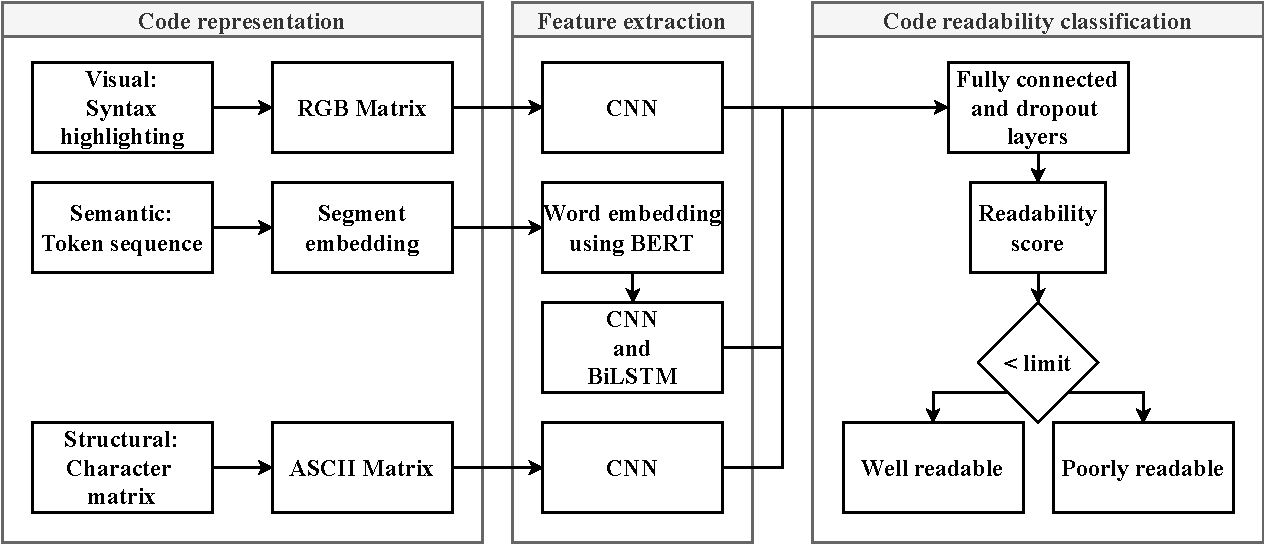
\includegraphics[width=\textwidth]{img/model_pipline.pdf}
		\caption{The architecture of the Towards model of \citeauthor{mi2022towards}~\cite{mi2022towards}.}
		\label{fig:model_pipeline}
	\end{figure}
	
	% Architecture
	The input for the model is a labeled dataset consisting of code snippets and their readability classes (poorly or well readable). In the code representation layer, the model generates three different code representations from each code snippet: A visual, a semantic, and a structural representation. 
	
	% Architecture: Visual embedding
	For the visual representation, the syntax of the code is highlighted. Therefore \citeauthor{mi2022towards} assigned each type of syntactic element a color (\autoref{tab:model-colors}). Instead of highlighting the words in the respective color, as done by an IDE, the words are replaced by color blocks instead (\autoref{fig:visual_encoding}). \citeauthor{mi2022towards} used Eclipse\curl{https://www.eclipse.org/}{2024-03-02} to highlight the code snippets and then took screenshots to obtain a RGB Matrix~\cite{mi2022towards}.
		
	\begin{table}[tb]
		\centering
		\caption{The color encoding used by the visual component of the Towards model~\cite{mi2022towards}.}
		\label{tab:model-colors}
		\begin{tabular}{lll}
			\toprule
			Element & Color & Hex Code \\
			\midrule
			Comment & \cellcolor{CommentColor} & \texttt{\#006200} \\
			Keyword & \cellcolor{KeywordColor} & \texttt{\#fa0200} \\
			Identifier & \cellcolor{IdentifierColor} & \texttt{\#01ffff} \\
			Literal & \cellcolor{LiteralColor} & \texttt{\#01ffff} \\
			Punctuation & \cellcolor{PunctuationColor} & \texttt{\#fefa01} \\
			Operator & \cellcolor{OperatorColor} & \texttt{\#fefa01} \\
			Generics & \cellcolor{GenericsColor} & \texttt{\#fefa01} \\
			Whitespace & \cellcolor{WhitespaceColor} & \texttt{\#ffffff} \\
			%			Unknown & \cellcolor{UnknownColor} & \texttt{\#ffffff} \\
			\bottomrule
		\end{tabular}
	\end{table}
	
%	\begin{listing}
%		\begin{minted}[linenos, frame=lines, framesep=2mm]{Java}
%    		/**
%			* Quits the application without any questions.
%			*/
%			public void quit() {
%				getConnectController().quitGame(true);
%				if (!windowed) {
%					gd.setFullScreenWindow(null);
%				}
%				System.exit(0);
%		\end{minted}
%		\label{lst:rdh-config-file}
%	\end{listing}
%	
%	\begin{figure}
%		\centering
%		
\includegraphics[width=\textwidth]{img/visual_encoding.png}
%		\caption{An example for a visual encoding of a code snippet.}
%		\label{fig:visual_encoding}
%	\end{figure}
	
	\begin{figure}
%		\begin{subfigure}{0.48\linewidth}
%			\begin{minted}[linenos, frame=lines, framesep=2mm]{Java}
%				// A method for counting
%				public void getNumber(){
%					int count = 0;
%					while(count < 10){
%						count++;
%					}
%				}
%			\end{minted}
%			\caption{An exemplary Java code snippet.}
%			\label{lst:java_code}
%		\end{subfigure}
		\begin{subfigure}[t]{0.48\textwidth}
			\centering
			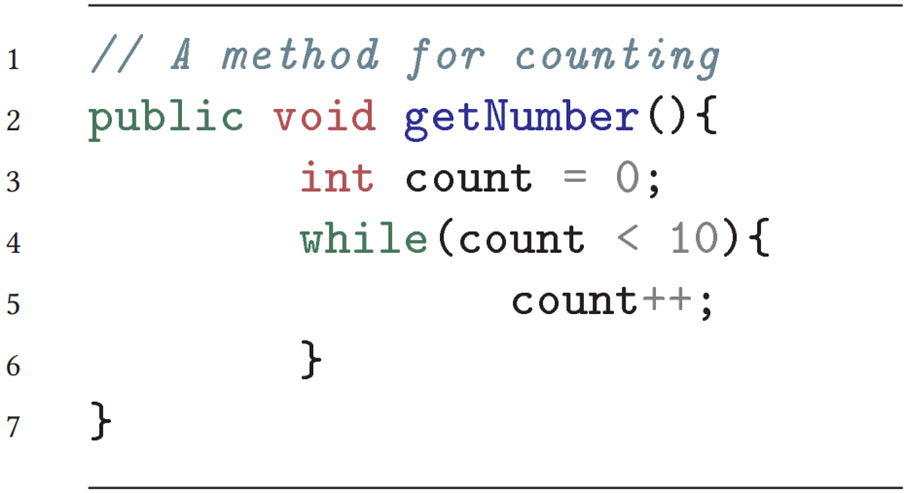
\includegraphics[width=\textwidth]{img/visual_encoding_code.png}
			\caption{An exemplary Java code snippet.}
			\label{lst:java_code}
		\end{subfigure}
		\begin{subfigure}[t]{0.48\textwidth}
			\centering
			
\includegraphics[width=\textwidth]{img/visual_encoding.png}
			\caption{The visual encoding of the code snippet in \autoref{lst:java_code}.}
			\label{fig:visual_encoding}
		\end{subfigure}
		\caption{A code snippet and its visual encoding.}
		\label{fig:visual_encoding_combined}
	\end{figure}
	
	% Architecture: Segment embedding
	For the semantic representation, we split the code into tokens (e.g., keywords and operators) and use BERT~\cite{devlin2018bert} to embed each token as a vector~\cite{mi2022towards}.
	
	% Architecture: Structural embedding
	For the structural representation, we split the code into characters and convert each into its ASCII value to obtain an ASCII matrix~\cite{mi2022towards}.
	
	% Architecture: Feature extraction (CNNs)
	The model takes the three representations as input. We perform feature extraction on the RGB matrix and the ASCII matrix using a CNN for each. Each of the CNNs consists of multiple convolution and max pooling layers and a single flatten layer~\cite{mi2022towards}. 
	
	% Architecture: Feature extraction Bidirectional LSTM
	On the token embedding the model performs feature extraction using a BERT embedding layer, convolution layers, a max pooling layer, and a Bidirectional LSTM (BiLSTM)~\cite{mi2022towards}.
	
	% Architecture: Classification
	After extracting the features from the three individual representations the output is merged and used as input for the final step: code readability classification. In this step, the model consists of multiple fully connected layers and a dropout layer. The output is a single value, namely the readability score. If the score is above a certain threshold, we classify the input as well readable, otherwise it is poorly readable~\cite{mi2022towards}.
	
	% Different: Model
	We implemented this model as described by \citeauthor{mi2022towards}~\cite{mi2022towards} with a few adjustments:
	In contrast to the publicly available code of \citeauthor{mi2022towards}\curl{https://github.com/swy0601/Readability-Features}{2024-02-20}, our model includes (batch) encoders required for the model to be trained on new data and to perform the prediction task for new code snippets. In addition, our model supports fine-tuning by freezing certain layers as well as storing intermediate results, such as the encoded dataset. During the evaluation, the model returns the evaluation statistics as a JSON file.
	
	% Different: Image encoding
	We made a further adjustment to the image encoding. To automate the generation of visual encodings we propose a different approach leading to a similar result. You can find an overview of our approach in \autoref{fig:visual_encoding_pipline}.
	
	\begin{figure}
		\centering
		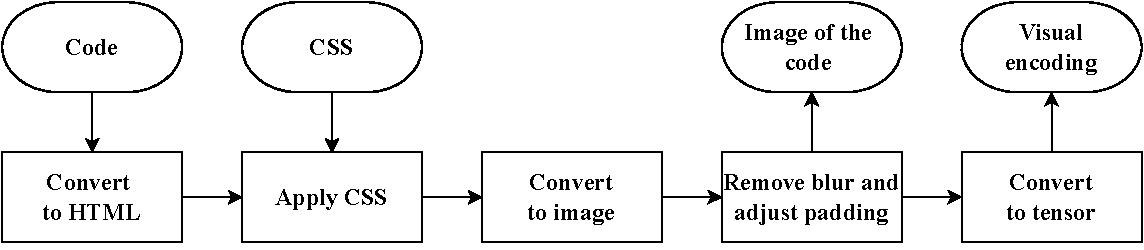
\includegraphics[width=\textwidth]{img/visual_encoding_pipline.pdf}
		\caption{The steps to automatically, visually encode code.}
		\label{fig:visual_encoding_pipline}
	\end{figure}
	
	In the first step, we use Imgkit\curl{https://pypi.org/project/imgkit/}{2024-03-02} to convert the code to HTML. Thereby, an HTML class is assigned to each type of syntactic element. Next, we apply syntax highlighting using a CSS style sheet (\Cref{appendix:model-visual-colors}). In the third step, we use pygments\curl{https://pygments.org/}{2024-03-02} to convert the HTML with the applied CSS to an image. We use pillow\curl{https://pypi.org/project/pillow/}{2024-03-02} to remove blur and adjust the padding of the image. Finally, we load the image using opencv-python\curl{https://pypi.org/project/opencv-python/}{2024-03-02} which allows us to convert the image to an RGB tensor that is suitable as a model input.
	The advantages of our approach are that it is fully automated and that the used colors can be adjusted easily via the CSS style sheet (\Cref{appendix:model-visual-colors}).
	
	% Problems
	During implementation, we encountered the following potential problem with the model:
	The token length for the BERT encoding (BERT-base-cased\curl{https://huggingface.co/google-bert/bert-base-cased}{2024-02-20}) used in the model is 100. We take a look at what implications this has, and therefore we first need to look at what a token comprises. In addition to special tokens that mark the beginning \textit{[CLS]} and the end \textit{[SEP]} of the input, each word represents a token. Furthermore, each special character is also represented by its own token. 
	Special characters are slashes~(\textbf{/}), parentheses~(\textbf{(},~\textbf{)},~\textbf{\{},~\textbf{\}}), commas~(\textbf{,}), semicolons~(\textbf{;}), arithmetic signs~(\textbf{=},~\textbf{<},~\textbf{>}) and many more.
	Java identifiers are split into several tokens according to the convention of upper and lower case. If an identifier is not present in the model's vocabulary, the tokenizer splits it further into sub-identifiers or characters that are in the vocabulary. 
	For example in \autoref{lst:print-greeting}, Line 6, the word \textquote{int} is split into the tokens \textquote{in} and \textquote{t} as \textquote{int} is not part of the vocabulary of BERT-base-cased.

	\begin{listing}[p]
		\begin{sublisting}{\linewidth}
			\begin{minted}[linenos, frame=lines, framesep=2mm]{Java}
				/**
				* This method determines the sign of a given number and prints a corresponding message.
				*
				* @param number The input number to be checked.
				*/
				public static void checkNumberSign(int number) {
					if (number > 0) {
						System.out.println("Number is positive");
					} else if (number < 0) {
						System.out.println("Number is negative");
					} else {
						System.out.println("Number is zero");
					}
				}
			\end{minted}
			\caption{An example of a simple and well readable Java method.}
			\label{lst:print-greeting-a}
		\end{sublisting}
		
		\begin{sublisting}{\linewidth}
			\begin{minted}[linenos, frame=lines, framesep=2mm]{Java}
				[CLS] / * *
				* This method determines the sign of a given number and prints a corresponding message .
				*
				* @ para m number The input number to be checked .
				* /
				public static void print S ign ( in t number ) {
				if ( number > 0 ) {
				System . out . print ln ( " Number is positive " ) ;
				} else if ( number < 0 ) {
				System . out . print ln ( " Number is negative " ) ;
				} else {
				System . out . print [SEP]
			\end{minted}
			\caption{The encoded-and-decoded variant of \autoref{lst:print-greeting-a} using BERT-base-cased with a limit of 100 tokens. Space characters separate the tokens. Newlines are preserved for readability.}
			\label{lst:print-greeting-b}
		\end{sublisting}
		\caption{A Java method and its encoded-and-decoded variant.}
		\label{lst:print-greeting}
	\end{listing}
	
	Consider the method from \autoref{lst:print-greeting-a}. With a token limit of 100, the last encoded token is the last \textit{print} in Line 12. Everything that comes after this is not encoded, which means that the information is lost for the semantic part of the model. Summarized, the model of \citeauthor{mi2022towards} only considers the first few lines of code snippets in its semantic component.
	
	The visual and structural encoders have similar limitations but to a smaller extent. The structural encoder encodes the first 50 lines of each code snippet and the visual encoder encodes the first 43 lines. While the constraints for these two encoders seem to be long enough to fully capture most code snippets, the semantic encoder seems to be too limited to do so in many cases.

	Although we want to point out these limitations, we retain them in order to make our results comparable with those of \citeauthor{mi2022towards} and thus enable a fair comparison of the datasets.
	
%	Our code is publicly available on GitHub\curl{https://github.com/LuKrO2011/master-thesis}{2024-03-21}.
	
%	You can find an overview over all programs used to create the merged dataset, the mined-and-modified dataset, the model and all our evaluation results in \autoref{fig:scripts_pipline}.
	
%	\begin{figure}[tb]
%		\centering
%		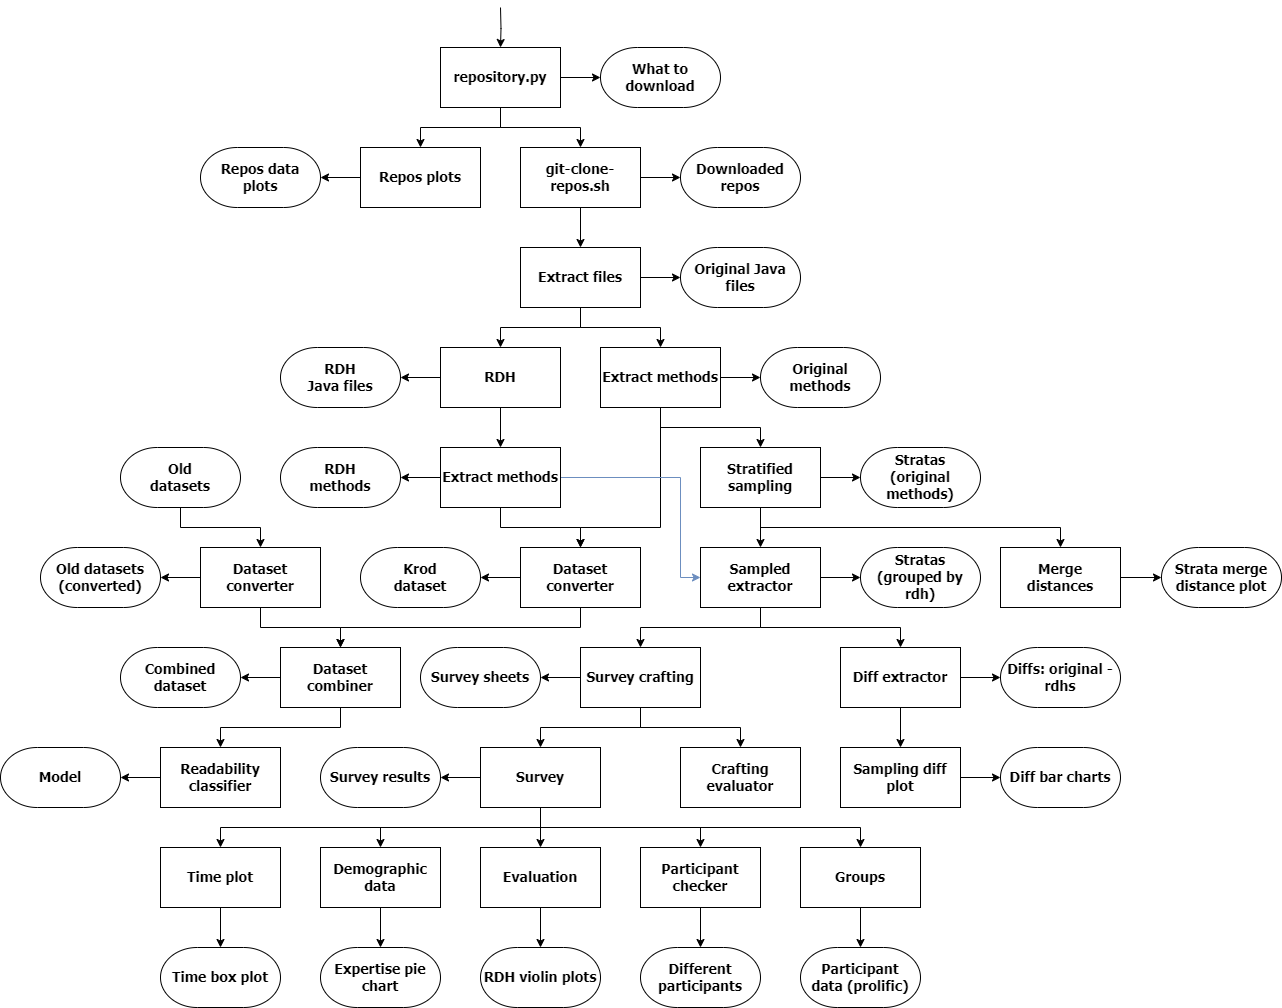
\includegraphics[width=\textwidth]{img/scripts_pipeline.png}
%		\caption{The used scripts and their output.}
%		\label{fig:scripts_pipline}
%	\end{figure}
%	
	
\chapter{Evaluation} \label{Evaluation}
	We tested the mined-and-modified dataset in two ways. We conducted a user study and evaluated the impact of using the dataset for the Towards model of \citeauthor{mi2022towards}~\cite{mi2022towards}. In detail, we answer the following questions with both experiments:
		
%	% User study
%	We are conducting a user study to determine the quality of the new dataset. In detail the aim of the user study is to answer the following key questions:
	\begin{enumerate}
		\item Does the well-readable-assumption (\Cref{well-readable-assumption}) hold?
		\item Does the poorly-readable-assumption (\Cref{poorly-readable-assumption}) hold?
	\end{enumerate}
	
	% Assumptions
	Our assumptions are as follows:
	\begin{enumerate}[label={Assumption \arabic*},ref={\arabic*},leftmargin=*]
		\item \label[assumption]{well-readable-assumption} \textbf{(well-readable-assumption)} The selected repositories contain mostly well readable code.
		\item \label[assumption]{poorly-readable-assumption} \textbf{(poorly-readable-assumption)} After applying \rdh, the code is poorly readable.
	\end{enumerate}
	
	% RQs
	Therefore, we come up with the following research questions:
	
	\begin{resq} \label[rq]{mined-well} \textbf{(mined-well)} Can automatically mined code be assumed to be well readable?\end{resq} 
	In our new approach for generating training data, we assume that the code from repositories is well readable under certain conditions (\Cref{well-readable-assumption}). We want to check whether that holds. To answer this question we use the results of the user study.
	
	\begin{resq} \label[rq]{modified-poor} \textbf{(modified-poor)} Can poorly readable code be generated from well readable code?\end{resq} 
	It is not sufficient to have only well readable code for training a classifier. We also need poorly readable code. Therefore, we try to generate such code from the well readable code. We investigate whether this is possible in principle and whether \rdh (\Cref{REDEC}) can achieve this.
	
	The modifications \rdh applies to the source code are heuristics. To answer whether the generated code is actually poorly readable (\Cref{poorly-readable-assumption}) we utilize the results of the user study.
	
	%	\begin{resq} \textbf{(best-heuristics)} Which heuristics are best to generate poorly readable code from well readable code?\end{resq} \label{best-heuristic}
	%	We want to compare the modifications of the proposed heuristics for generating poorly readable code to each other. Therefore we will use the results of the user study (\autoref{user-study}).
	
	\begin{resq} \label[rq]{new-data} \textbf{(new-data)} To what extent can the new data improve existing code readability classification models?\end{resq} 
	Previous research shows that Deep Learning models get better the more training data is available~\cite{hestness2017deep}. This applies under the assumption that the quality of the data is the same or at least similar. We want to check if the quality of our new data is sufficient for improving the deep learning-based readability classifier of \citeauthor{mi2022towards}~\cite{mi2022towards}. We train their proposed model with combinations of the merged and the mined-and-modified dataset and compare the results.

\section{Survey} \label{Survey}
	This section is divided into two parts: The pilot survey, which was used to improve the main survey pre-launch, and the main survey, which was used to answer our research questions and to craft our dataset.
	
\subsection{Pilot Survey} \label{Pilot Survey}
	
	% Experimental setup
	\textbf{1. Experimental setup:}
	We manually sampled 20 code snippets across all strata but mainly from Stratum 1 and Stratum 3 due to reasons mentioned in \Cref{Construction of Questionnaires}. From January 6 to 14, 2024 ten people took part in the survey. Eight of them were students and two of them worked in the industry. All of them have computer science knowledge. They were not paid for participating in the survey. Additionally to rating 20 code snippets, the participants were also asked to answer further questions to provide feedback about the survey:
	
	% Questions
%	They were asked the following additional questions:
	\begin{enumerate}
		\item \textit{Short answer}: How long did it take you to complete the survey?
		\item \textit{Single choice (1 (very unclear) to 5 (very clear)):} How clear was your task?
		\item \textit{Long answer:} What problems were with the task? If there were none, leave blank.
		\item \textit{Long answer:} What problems were there with the survey tool? If there were none, leave blank.
		\item \textit{Long answer:} What improvements would you make to the survey? If none, leave blank.
		\item \textit{Long answer:} Do you have any other feedback? If none, leave blank.
	\end{enumerate}
	
%	The participants answers can be found in \Cref{appendix:pilot-survey-feedback}.
	
	% Usage
%	The feedback of the pilot survey was used in the following ways to prepare the Prolific study:
%	\begin{itemize}
%		\item To adjust the survey texts and questions
%		\item To estimate how long completion of one questionnaire will take
%		\item To adjust the \rdh settings
%		\item To discover problems with the survey tool
%		\item To discover fundamental problems with the dataset
%	\end{itemize}
	
	% Threats
	\textbf{2. Threats to Validity:}
	The threats regarding the pilot survey are as follows:
	
	\textit{External Validity:}
	We did not sample the Java snippets for rating in a specific or automated way, so there is a selection bias. Participants coming from a private environment further exacerbate this bias. Due to both, the results do not generalize.
	
	\textit{Internal Validity:}	
	Ten people took part in the pilot survey. Due to the small number of participants, it is not possible to draw reliable conclusions about the strata or \rdh configurations. 	
	However, the results are sufficient to provide an indication.
	%	We adjusted the survey instructions, explanations, and questions after the conduction of the survey, which might influence the ratings of the participants.
	
	\textit{Construct Validity:}
	%	We adjusted the survey instructions, explanations, and questions after the conduction of the survey, which might influence the ratings of the participants.
	%	We do not define readability for the raters, as there are various definitions which slightly defer from each other (\Cref{Code Readability}). Instead we intuitive
	The accuracy of the participants' ratings for the code snippets is uncertain. We see no incentive for participants to intentionally provide incorrect ratings. We come to the conclusion to measure readability.
	
	None of the mentioned threats has any impact as we do not use the results of this survey for the evaluation of our dataset generation approach.
	The intention of the pilot survey was rather to prepare for the main survey.
	
	% Results
	\textbf{3. Results:}
	We analyze the results of the pilot survey regarding three aspects: the time it took to complete the survey, the feedback from the participants, and the ratings of the selected code snippets.
	
	\textit{Completion Time:} 
	\autoref{fig:survey_times} shows the time it took the participants to complete the pilot survey and thus to rate 20 code snippets according to their readability.
	The fastest participant completed the survey in 7 minutes and 35 seconds, while the slowest participant took 18 minutes. 
	Both, the average value and the mean value, are around 12 minutes. The boxplot (\autoref{fig:survey_times}) shows that the times are close together and there are no outliers in the time taken.
	We suspect that the participants in the pilot survey put more effort into completing the survey as we know them personally. 
	Other participants may not make as much effort, so we set the time estimation for a questionnaire below average at 10 minutes.
		
%	\begin{figure}[tb]
%		\centering
%		\begin{subfigure}{0.49\textwidth}
%			\centering
%			\includegraphics[width=\linewidth]{img/pilot_survey_time_box.png}
%			\caption{Time required by the participants to complete the pilot survey.}
%			\label{fig:pilot_survey_time_box.png}
%		\end{subfigure}
%		\hfill
%		\begin{subfigure}{0.49\textwidth}
%			\centering
%			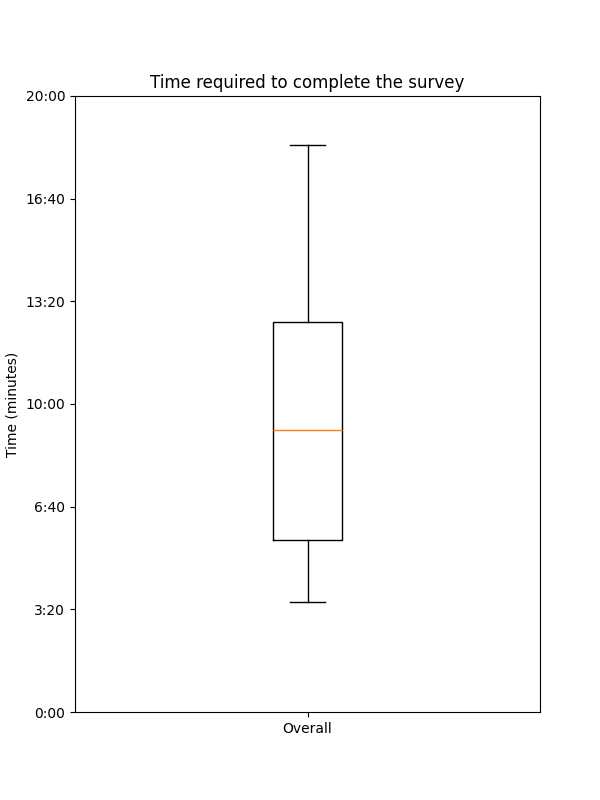
\includegraphics[width=\linewidth]{img/survey_time_box.png}
%			\caption{Time required by the participants to complete the Prolific survey.}
%			\label{fig:survey_time_box}
%		\end{subfigure}
%		\caption{Time required to complete the surveys.}
%		\label{fig:survey_time_both}
%	\end{figure}

	\begin{figure}[tb]
		\centering
		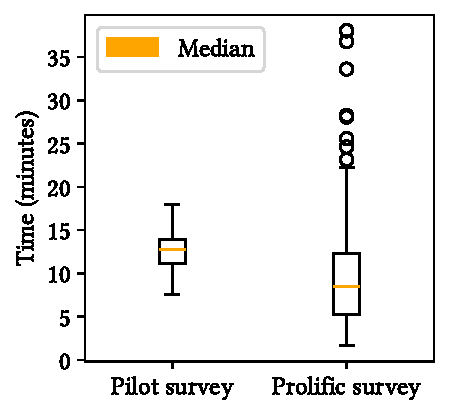
\includegraphics[width=0.5\textwidth]{img/survey_times.pdf}
		\caption{Time required to complete a questionnaire.}
		\label{fig:survey_times}
	\end{figure}
		
	\textit{Participant Feedback:}
	All feedback from the participants regarding the pilot survey is listed in \Cref{appendix:pilot-survey-feedback}.
	Most of the problems that occurred were due to the survey tool (e.g.: \textquote{I also felt that I should use the drop-down menu at the top left.}).
	%	Zusammengefasst:
	%	Feature Request: "You're done! Thank you for your participation!" - message at the end
	%	Feature Request: Hide comment fields
	%	Feature Request: Predefine code parser (per survey/snippet) and hide selection during survey for participants
	%	Feature Request: Possibility to show a hint or the task description again during the survey
	Some of the feedback was regarding fully qualified class names, such as \textquote{Java.io.InputStream}. We noticed that the Pretty Printer of the \rdh tool specified each imported method or class with its fully specified classifier. For example, instead of \textquote{InputStream}, \textquote{Java.io.InputStream} was written in the \rdh code snippets. This gave the participants the feeling that the code was not written by a human and drastically reduced readability. Therefore we adapted the \rdh tool to print the shorter name.
	%	A potential drawback is that it can no longer be assumed that the generated code will compile and behave exactly like the original. However, the compilation-property is lost anyway during method extraction.
	
		%	\begin{table}[htbp]
		%		\centering
		%		\begin{tabular}{llp{6cm}c}
			%			\toprule
			%			\textbf{Stratum} & \textbf{\rdh} & \textbf{File} & \textbf{Score} \\
			%			\midrule
			%			stratum\_0 & spaces-few & \seqsplit{hadoop\_FilePosition.Java\_bufferFullyRead.Java} & 3 \\
			%			stratum\_0 & tabs-few & \seqsplit{hadoop\_DataNodeFaultInjector.Java\_delayWriteToDisk.Java} & 4,3 \\
			%			stratum\_1 & all & \seqsplit{hudi\_HoodieMultiTableStreamer.Java\_populateTableExecutionContextList.Java} & 1,2 \\
			%			stratum\_1 & all2 & \seqsplit{flink\_SSLUtils.Java\_createInternalNettySSLContext.Java} & 1,3 \\
			%			stratum\_1 & newlines-few & \seqsplit{hudi\_Pipelines.Java\_hoodieStreamWrite.Java} & 1,7 \\
			%			stratum\_1 & spaces-many & \seqsplit{hadoop\_ActiveAuditManagerS3A.Java\_createExecutionInterceptors.Java} & 2,1 \\
			%			stratum\_1 & tabs-few & \seqsplit{hbase\_ZKMainServer.Java\_main.Java} & 2,2 \\
			%			stratum\_1 & tabs-many & \seqsplit{flink\_HiveParserSemanticAnalyzer.Java\_findCTEFromName.Java} & 2,2 \\
			%			stratum\_1 & misc & \seqsplit{hbase\_Encryption.Java\_decryptWithSubjectKey.Java} & 2,4 \\
			%			stratum\_1 & spaces-few & \seqsplit{hbase\_HBaseZKTestingUtility.Java\_startMiniZKCluster.Java} & 2,6 \\
			%			stratum\_1 & newlines-many & \seqsplit{pulsar\_LoadSimulationController.Java\_writeProducerOptions.Java} & 2,9 \\
			%			stratum\_1 & all-weak-r & \seqsplit{hadoop\_SingleFilePerBlockCache.Java\_getIntList.Java} & 3 \\
			%			stratum\_1 & comments-remove & \seqsplit{flink\_MemorySegment.Java\_get.Java} & 3,1 \\
			%			stratum\_1 & methods & \seqsplit{flink\_HiveParserSemanticAnalyzer.Java\_processPTFSource.Java} & 3,7 \\
			%			stratum\_2 & newlines-few & \seqsplit{zxing\_ModulusPoly.Java\_isZero.Java} & 2,4 \\
			%			stratum\_2 & methods & \seqsplit{hibernate-validator\_PESELValidator.Java\_year.Java} & 3,7 \\
			%			stratum\_2 & tabs-few & \seqsplit{framework\_WindowMoveListener.Java\_getTicketNumber.Java} & 3,8 \\
			%			stratum\_3 & tabs-many & \seqsplit{hadoop\_S3AInputPolicy.Java\_getPolicy.Java} & 1,7 \\
			%			stratum\_3 & newlines-many & \seqsplit{hadoop\_CompressionCodec.Java\_createInputStreamWithCodecPool.Java} & 3,3 \\
			%			stratum\_3 & methods & \seqsplit{hbase\_PreviousBlockCompressionRatePredicator.Java\_updateLatestBlockSizes.Java} & 4,6 \\
			%			\bottomrule
			%		\end{tabular}
		%		\caption{Data with Highlighted Row}
		%		\label{tab:pilot_survey_results}
		%	\end{table}
	
	%	\begin{table}[htbp]
		%		\centering
		%		\caption{Mean score ratings for the pilot survey}
		%		\vspace{8pt}
		%		\label{tab:pilot_survey_results}
		%		\begin{tabular}{llp{6cm}r}
			%			\toprule
			%			\textbf{Stratum} & \textbf{Feature} & \textbf{File} & \textbf{Score} \\
			%			\midrule
			%			stratum\_3 & methods & \seqsplit{hbase\_PreviousBlockCompressionRatePredicator.Java\_updateLatestBlockSizes.Java} & 4,6 \\
			%			stratum\_0 & tabs-few & \seqsplit{hadoop\_DataNodeFaultInjector.Java\_delayWriteToDisk.Java} & 4,3 \\
			%			stratum\_2 & tabs-few & \seqsplit{framework\_WindowMoveListener.Java\_getTicketNumber.Java} & 3,8 \\
			%			stratum\_1 & methods & \seqsplit{flink\_HiveParserSemanticAnalyzer.Java\_processPTFSource.Java} & 3,7 \\
			%			stratum\_2 & methods & \seqsplit{hibernate-validator\_PESELValidator.Java\_year.Java} & 3,7 \\
			%			stratum\_3 & newlines-many & \seqsplit{hadoop\_CompressionCodec.Java\_createInputStreamWithCodecPool.Java} & 3,3 \\
			%			stratum\_1 & comments-remove & \seqsplit{flink\_MemorySegment.Java\_get.Java} & 3,1 \\
			%			stratum\_0 & spaces-few & \seqsplit{hadoop\_FilePosition.Java\_bufferFullyRead.Java} & 3,0 \\
			%			stratum\_1 & all-weak-r & \seqsplit{hadoop\_SingleFilePerBlockCache.Java\_getIntList.Java} & 3,0 \\
			%			stratum\_1 & newlines-many & \seqsplit{pulsar\_LoadSimulationController.Java\_writeProducerOptions.Java} & 2,9 \\
			%			stratum\_1 & spaces-few & \seqsplit{hbase\_HBaseZKTestingUtility.Java\_startMiniZKCluster.Java} & 2,6 \\
			%			stratum\_1 & misc & \seqsplit{hbase\_Encryption.Java\_decryptWithSubjectKey.Java} & 2,4 \\
			%			stratum\_2 & newlines-few & \seqsplit{zxing\_ModulusPoly.Java\_isZero.Java} & 2,4 \\
			%			stratum\_1 & tabs-few & \seqsplit{hbase\_ZKMainServer.Java\_main.Java} & 2,2 \\
			%			stratum\_1 & tabs-many & \seqsplit{flink\_HiveParserSemanticAnalyzer.Java\_findCTEFromName.Java} & 2,2 \\
			%			stratum\_1 & spaces-many & \seqsplit{hadoop\_ActiveAuditManagerS3A.Java\_createExecutionInterceptors.Java} & 2,1 \\
			%			stratum\_1 & newlines-few & \seqsplit{hudi\_Pipelines.Java\_hoodieStreamWrite.Java} & 1,7 \\
			%			stratum\_3 & tabs-many & \seqsplit{hadoop\_S3AInputPolicy.Java\_getPolicy.Java} & 1,7 \\
			%			stratum\_1 & all2 & \seqsplit{flink\_SSLUtils.Java\_createInternalNettySSLContext.Java} & 1,3 \\
			%			stratum\_1 & all & \seqsplit{hudi\_HoodieMultiTableStreamer.Java\_populateTableExecutionContextList.Java} & 1,2 \\
			%			\bottomrule
			%		\end{tabular}
		%	\end{table}
	
	\begin{table}[tb]
		\centering
		\caption{Mean score ratings for the pilot survey. 
%			\texttt{all2} and \texttt{all4} consist similar to \texttt{all7} of all configurations but with $/2$ and $/4$ for all probabilities.
		}
		\label{tab:pilot_survey_results}
		\begin{tabular}{llr}
			\toprule
			Stratum & \rdh configuration & Score \\
			\midrule
			Stratum 3 & original & 4.6 \\
			Stratum 0 & tabs-few & 4.3 \\
			Stratum 2 & tabs-few & 3.8 \\
			Stratum 1 & original & 3.7 \\
			Stratum 2 & original & 3.7 \\
			Stratum 3 & newlines-many & 3.3 \\
			Stratum 1 & comments-remove & 3.1 \\
			Stratum 0 & spaces-few & 3.0 \\
			Stratum 1 & all4 & 3.0 \\
			Stratum 1 & newlines-many & 2.9 \\
			Stratum 1 & spaces-few & 2.6 \\
			Stratum 1 & misc & 2.4 \\
			Stratum 2 & newlines-few & 2.4 \\
			Stratum 1 & tabs-few & 2.2 \\
			Stratum 1 & tabs-many & 2.2 \\
			Stratum 1 & spaces-many & 2.1 \\
			Stratum 1 & newlines-few & 1.7 \\
			Stratum 3 & tabs-many & 1.7 \\
			Stratum 1 & all2 & 1.3 \\
			Stratum 1 & all & 1.2 \\
			\bottomrule
		\end{tabular}
	\end{table}
	
	\textit{Ratings:}
	We adjusted the \rdh configurations. The rating for the last places (\autoref{tab:pilot_survey_results}), such as \textit{1.2} for \textit{Stratum 1 - all}, suggest that these code snippets were particularly poorly readable. 
	Thus, we re-examined the \rdh configurations and found that some of them are over-configured. This not only affects their readability but also makes them look as if they were not written by human hands. Therefore, we reduced the probabilities for these configurations.
	
	After adjusting the \rdh configurations and the survey tool according to the feedback, we launched the Prolific survey.

\subsection{Prolific Survey} \label{Prolific Survey}
	In this section, we summarize the results of the main survey conducted via Prolific\curl{https://app.prolific.com/}{2024-02-21}.
		
\textbf{1. Experimental setup:}
	We conducted the survey using Tien Duc Nguyen's Code Annotation Tool (\autoref{fig:survey_tool}) along with the platform Prolific for the recruitment and payment of participants.
	The survey was conducted between January 31 and February 7, 2024. A total of 221 participants took part. 11 participants answered each of the 20 questionnaires (similar to the survey of \citeauthor{scalabrino2018comprehensive}~\cite{scalabrino2018comprehensive}). In one survey, we assigned one more participant by mistake. We include his results in the evaluation. We estimated the time to complete one questionnaire at 10 minutes (\Cref{Pilot Survey}). Prolific set the maximum time allowed at 44 minutes. Participants who took longer received a time-out.
	%	According to an online calculator\footnote{https://www.calculator.net/sample-size-calculator.html} 
	This results in a margin of error of 29.55\% at a confidence of 95\% for an individual snippet.
%	The margin of error is a statistic that indicates the amount of sampling error. The smaller the margin of error, the more certain it is that a survey result corresponds to the actual value. 
	A margin of error of 29.55\% means that the actual readability value of a code snippet varies by up to 29.55\% in both directions from the evaluation result.
	However, we aggregate over strata and multiple snippets later to reduce the margin of error.
	Each questionnaire consists of 20 code snippets. Consequently, 400 different code snippets are rated in total. The questionnaires were configured in a way that each participant could only take part in one of the questionnaires. You can find the texts for the survey in \Cref{appendix:prolific-survey-texts}. We crafted the questionnaires as described in \Cref{Construction of Questionnaires}.
		
	\begin{figure}[tb]
		\centering
		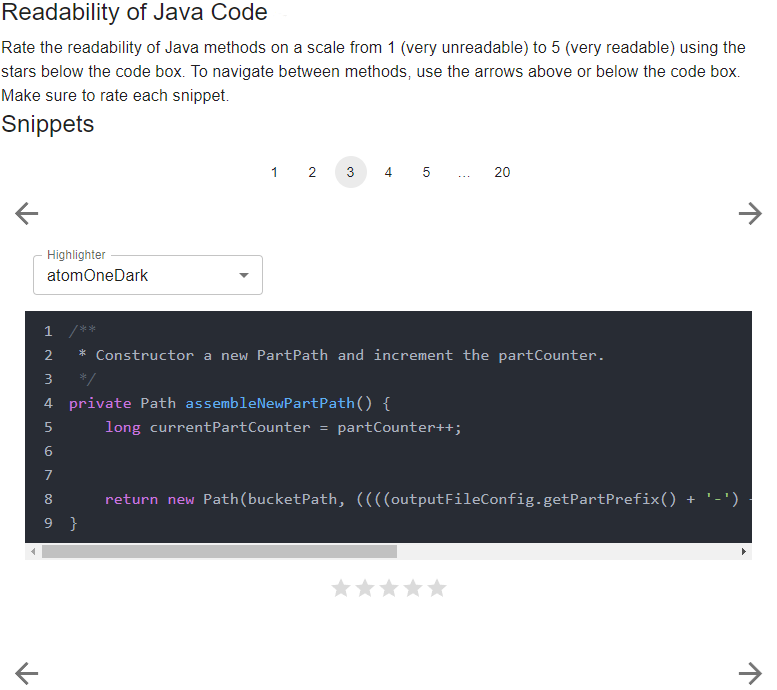
\includegraphics[width=\textwidth]{img/survey_tool.png}
		\caption{Tien Duc Nguyen's tool for rating a code snippet from the perspective of a survey participant.}
		\label{fig:survey_tool}
	\end{figure}

	% Target population
	The target population consists of Java programmers selected by Prolific. They may be students or work in industry. They can come from any country. Overall, there were no requirements other than familiarity with Java.
	
%	(see also \autoref{tab:prolific-audience}).
	
%	\begin{table}[tb]
%		\centering
%		\caption{Target population for the Prolific survey.}
%		\vspace{8pt}
%		\label{tab:prolific-audience}
%		\begin{tabular}{ll}
%			\toprule
%			Type & Target Population \\
%			\midrule
%			Target Audience      & Java programmers \\
%			Unit of Observation  & Java programmers \\
%			Unit of Analysis     & Java programmers \\
%			Search Unit          & Selected by Prolific (Programming Languages: Java)\\
%			Source of Sampling   & Prolific \\
%			\bottomrule
%		\end{tabular}
%	\end{table}
	
	% Internal/Research Questions
	The internal research questions are as follows:
	\begin{itemize}
		\item Does the well-readable-assumption (\Cref{well-readable-assumption}) hold?
		\item Does the poorly-readable-assumption (\Cref{poorly-readable-assumption}) hold?
	\end{itemize}
	
	The results of these questions are equally important, and thus none of them is prioritized over the other.
	To answer them, the assumptions	are considered as hypotheses along with the following associated null hypotheses:
	\begin{itemize}
		\item For \Cref{well-readable-assumption}: The mined code (original) is on average not better readable than the code from previous studies.
		\item For \Cref{poorly-readable-assumption}: The readability of modified code does not significantly deteriorate compared to the original code snippet.
	\end{itemize}
	
	% Questionnaire Attributes
	The survey neither contained demographic questions nor filter questions. Besides the readability questions, we asked each participant the following dependent question: \textquote{How would you describe your familiarity with Java?}. The participant could answer within a five-point Likert scale: expert (5), advanced (4), intermediate (3), beginner (2), novice (1).
	
\textbf{2. Threats to Validity:}
	We identified the following threats:
	
	\textit{External Validity:}
	Due to our questionnaire construction approach (\Cref{Construction of Questionnaires}), we have a larger proportion of code snippets from Stratum 1 and Stratum 3 (\Cref{Construction of Questionnaires}). While we argue that we avoided spending resources on labeling data that is likely not different from the original methods or rather uninteresting, this might also introduce statistical errors to our survey results.
	However, stratified sampling is well-defined and proven in practice. The approach ensures that our sample represents all parts of the population under investigation.
	Ensuring a well-defined target population is critical to the survey's quality.
	To mitigate the threat of an inadequately defined target population, we define it explicitly.
	
	\textit{Internal Validity:}	
	To prevent concluding from an insufficient number of responses, we scale our survey to an appropriate size. This guarantees that we collect a substantial volume of responses, allowing for robust statistical analysis.
	Survey participants are paid for taking part and completing a questionnaire. However, they receive the same amount of money regardless of their speed. Therefore, they receive more pay per minute if they hurry. This could have an impact on the accuracy with which they scored the code snippets. A comparison between the time required by a participant for a pilot questionnaire and a Prolific questionnaire (\autoref{fig:survey_times}) supports this argument. Especially the ratings of participants requiring less than 3 minutes (\autoref{fig:survey_time_less_than_180}) to complete a questionnaire could have a negative impact on validity. 
	
	\textit{Construct Validity:}
	The accuracy of the participants' ratings for the code snippets is uncertain. Apart from the already mentioned aspect that participants might hurry, we see no incentive for participants to deliberately give false ratings. We come to the conclusion to measure readability.
	
\textbf{3. Results:}
	We analyze the results of the Prolific survey regarding three aspects: the time it took to complete the survey, the participants' familiarity with Java, and the ratings about the \rdh configurations.

	\textit{Completion time:}
	You can find an overview of the time that the participants required in \autoref{fig:survey_times} and \autoref{fig:survey_time_histogramm}.
	The fastest participant completed the survey in 1 minute and 39 seconds, while the slowest participant needed about 38 minutes. 
	The average time is 9 minutes and 45 seconds. The median time is 8 minutes and 30 seconds. The boxplot (\autoref{fig:survey_times}) shows that the completion times are not as close together as they are in the pilot survey. There are a couple of outliers.
	
	We pay attention to the number of participants who took less than 3 minutes to complete a questionnaire (\autoref{fig:survey_time_less_than_180}), as we assume that this is hardly possible without randomly selecting answers. In almost all questionnaires, the number of participants who took less than 3 minutes is either 0 or 1, while there is only one questionnaire where two participants took less than 3 minutes.
	Overall, there are only a few participants who took less than 3 minutes. We assume that most participants completed the survey with reasonable effort.
		
	\begin{figure}[tb]
		\centering
		\begin{subfigure}{0.49\textwidth}
			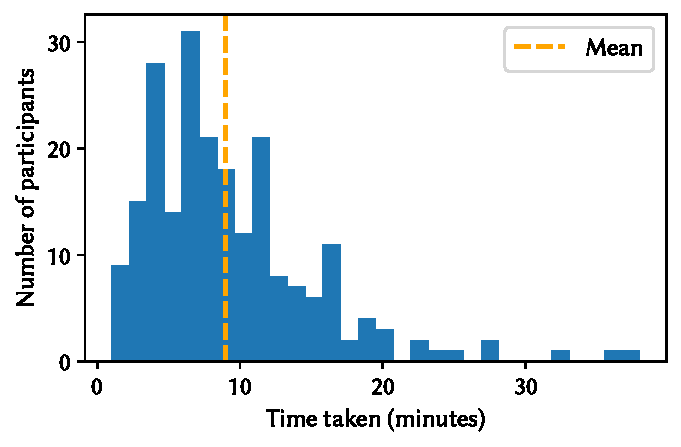
\includegraphics[width=\linewidth]{img/survey_time_histogramm.pdf}
			\caption{Time required by participants to complete the survey.}
			\label{fig:survey_time_histogramm}
		\end{subfigure}
		\hfill
		\begin{subfigure}{0.49\textwidth}
			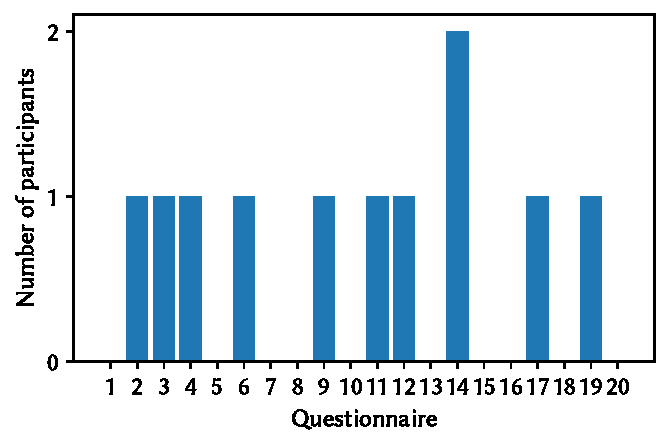
\includegraphics[width=\linewidth]{img/survey_time_less_than_180.pdf}
			\caption{Participants per questionnaire requiring less than 3 minutes.}
			\label{fig:survey_time_less_than_180}
		\end{subfigure}
		\caption{Time analysis of participants completing the Prolific survey.}
		\label{fig:survey_time_prolific}
	\end{figure}
	
	\textit{Familiarity with Java:}
%	The participants' familiarity with Java is shown in \autoref{fig:survey_Java_familiarity_pie}. According to their own estimation, 44.8~\% of the participants are experts with Java. Another 44.8~\% of the participants are either advanced or intermediate. This high level of familiarity with Java suggests that the quality of the evaluations received is also high.
	\autoref{fig:survey_Java_familiarity_pie} shows the participants' familiarity with Java. According to their estimation, most participants (43.3~\%) have intermediate Java knowledge. 
	29.0~\% of the participants stated that they are either advanced or experts in Java. This high level of familiarity with Java suggests that the quality of the evaluations received is high.
	
	\begin{figure}[tb]
		\centering
		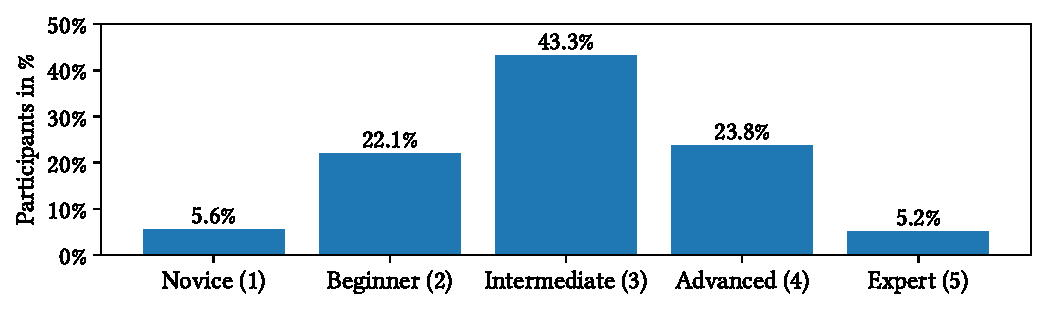
\includegraphics[width=\textwidth]{img/survey_java_familiarity_bar.pdf}
		\caption{Familiarity of Prolific survey participants with Java.}
		\label{fig:survey_Java_familiarity_pie}
	\end{figure}
		
	\textit{Ratings:}
	You can find the ratings for each \rdh configuration for all strata in \autoref{fig:survey_time_all}. We added the ratings of the merged dataset for comparison. \autoref{fig:survey_ratings_violin_all} visualizes the distribution of ratings for each score from 1 to 5. It also shows the mean value and mode of the ratings for each variant. To facilitate comparison with the original methods, the mean value of the ratings of the original methods across all variants is marked with a red dashed line. The original method and the \texttt{just-pretty-print} method are the most frequently rated with a score of 4 and their mean values of 3.69 and 3.67 are comparatively the highest.
		
	In line with our expectation, we see that the ratings for \nonet and \texttt{original} only differ by a negligible amount of 0.02. A Mann-Whitney-U-Test shows that the probability, that the difference between \nonet and \texttt{original} is due to random variation, is 92~\%.
%	There is no significant difference between the two, as a Mann-Whitney U test confirmed. The probability that the difference between \nonet and \texttt{original} is due to random variation is 92~\%. 
	Therefore, we are sure that not the Pretty Printer but the modifications caused the differences in readability.
	
	\begin{sloppypar}
	The violins of \autoref{fig:survey_ratings_violin_all} illustrate the distribution of the ratings in detail. Note that the evaluators were only able to rate the discrete values from 1 to 5. The deflections of the violins in between are for better visualization. The figure shows that for \texttt{original} and \texttt{just-pretty-print} most of the ratings are 3, 4, or 5. In addition, the violins of \texttt{merged} and \texttt{all7} look similar, with the latter having more 2 ratings. The violins of \texttt{newlines-many}, \texttt{rename} and \texttt{spaces-many} show more better (3, 4 and 5) and less worse (1 and 2) ratings than the ones of \texttt{comments-remove}, \texttt{newlines-instead-of-space}, \texttt{newlines-few} and \texttt{tabs}.
	\end{sloppypar}
		
	\autoref{fig:survey_ratings_violin_all} also shows that the mean value of the original methods is 3.69 and the mean value of the merged dataset is 3.34. The difference of 0.35 has statistical significance:
	We perform a Mann-Whitney-U-Test for the rating values of the 40 original code snippets of the mined-and-modified dataset against all rating values of the merged dataset. The resulting $p$ value is \num{1.11e-09}, which is far below the $5~\%=\num{5e-2}$ threshold and confirms statistical significance.
	
%	while for all7 it is 3.26	
%	We label each method in both groups with the corresponding mean score.

	\begin{summary}{\hyperref[mined-well]{RQ 1 - mined-well}}
		%		The readability ratings of code snippets mined from Github are not very accurate as we take the mean of all ratings for all methods and assign it to each snippet.
		The mean score for the \texttt{original} methods of the mined-and-modified dataset (3.69) is significantly larger than the mean score for all ratings in the merged dataset (3.34). Therefore we reject the null hypothesis and conclude that the well readable assumption (\Cref{well-readable-assumption}) holds.
		%		and answer the research question \ref{mined-well}: Yes, automatically selected code can be assumed to be well readable.
	\end{summary}
	
	\begin{figure}[p]
		\centering
		\begin{subfigure}{\linewidth}
			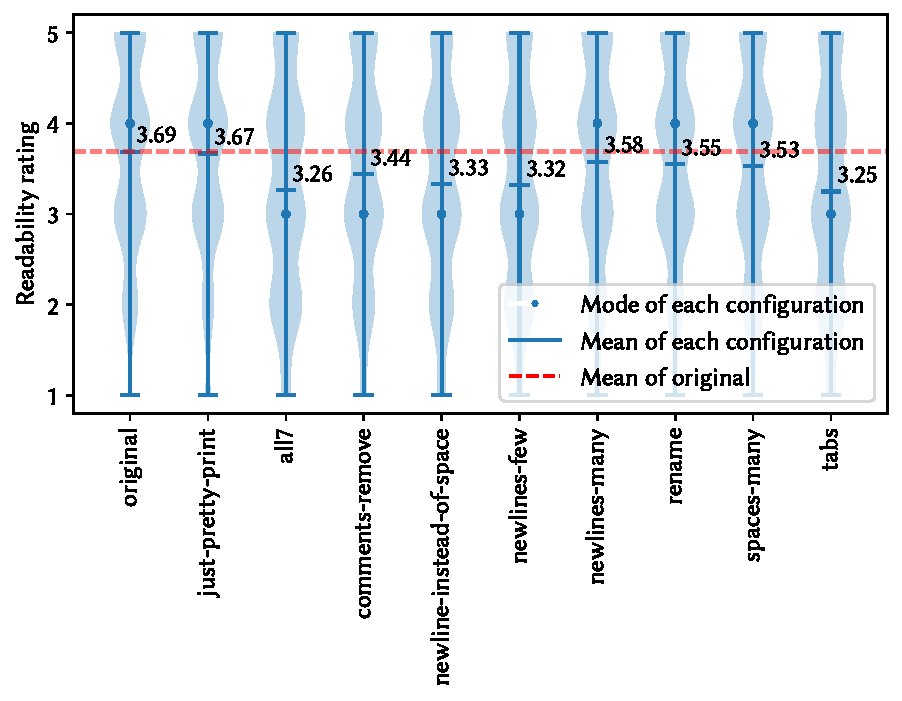
\includegraphics[width=0.9\textwidth]{img/survey_ratings_violin_all.pdf}
			\caption{Survey ratings for each \rdh configuration and all strata.}
			\label{fig:survey_ratings_violin_all}
		\end{subfigure}
		\hfill
		\begin{subfigure}{\textwidth}
			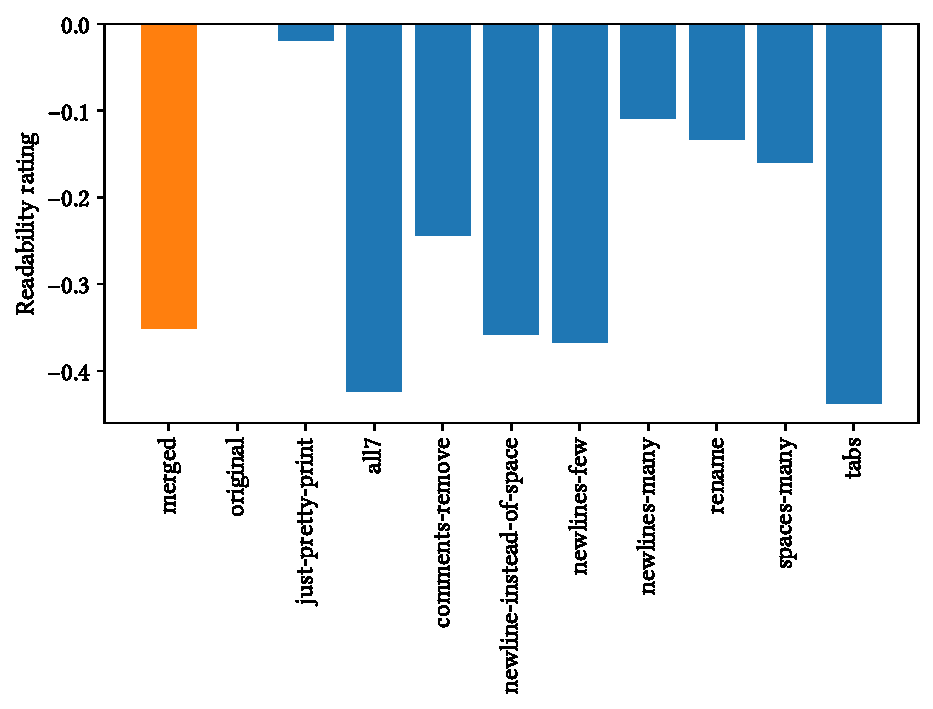
\includegraphics[width=0.9\linewidth]{img/survey_ratings_bar_all.pdf}
			\caption{Relative survey ratings for each \rdh configuration and all strata compared to all original methods.}
			\label{fig:survey_ratings_bar_all}
		\end{subfigure}
		\caption{Survey ratings for each \rdh configuration and all strata. Additionally, merged is added.}
		\label{fig:survey_time_all}
	\end{figure}
	
	\begin{sloppypar}
	\autoref{fig:survey_ratings_bar_all} shows the differences in mean values more precisely. \rdh reduces the readability for the configurations \texttt{all7}, \texttt{comments-remove}, \texttt{newlines-instead-of-space}, \texttt{newlines-few} and \texttt{tabs} the most. The tool also reduces readability for \texttt{newlines-many}, \texttt{rename}, and \texttt{spaces-many}, but not as much. 
	\end{sloppypar}
	To determine whether the deviations are statistically significant we utilize the Mann-Whitney-U-Test once more. We compare the ratings for all snippets for a \rdh configuration with the corresponding \nonet snippets. \autoref{tab:survey_statistical_evidence} shows the results.
	%	We do a statistical evaluation to find out whether the values could be random deviations or whether they are statistically significant (\autoref{tab:survey_statistical_evidence}).
	%	To answer our second research question, we analyzed whether the difference in ratings between the different \rdh configurations is statistically significant. 
	%	To do this, we used the Mann-Whitney U test to compare the ratings for all snippets for a \rdh configuration with the corresponding \nonet snippets. The results can be found in \autoref{tab:survey_statistical_evidence}.
	We can be sure that the scores of all methods except \texttt{newlines-many} and \texttt{rename} are indeed statistically different from the scores of \nonet. 
	
	If we consider binary readability classification and split the data into two classes (poorly readable: 1,2; well readable: 3-5) all but \texttt{rename} are statistically different from \nonet. This includes \texttt{newlines-many} ($p=0.035=3.5~\% < 5~\%$) for which we could not confirm statistical difference without binary classification.

	Besides \nonet, this leaves \texttt{rename} where we can not confirm statistical significance. Overall, we showed that \rdh reduces the readability of source code.

%	\begin{table}[h]
%		\centering
%		\caption{Mann-Whitney U test results of none against each \rdh}
%		\vspace{8pt}
%		\label{tab:survey_statistical_evidence}
%		\begin{tabular}{lS[table-format=1.2e-2]}\dfrac{Zähler}{Nenner}
%			\toprule
%			\textbf{Condition} & \textbf{$p$} \\
%			\midrule
%			None - Methods & \cellcolor{red!25}\num{9.22e-1} \\
%			None - Newlines Few & \cellcolor{green!25}\num{5.23e-6} \\
%			None - Spaces Many & \cellcolor{green!25}\num{4.07e-2} \\
%			None - Newlines Many & \cellcolor{red!25}\num{3.00e-1} \\
%			None - Comments Remove & \cellcolor{green!25}\num{3.64e-3} \\
%			None - Rename & \cellcolor{red!25}\num{9.90e-2} \\
%			None - Newline Instead Of Space & \cellcolor{green!25}\num{4.57e-6} \\
%			None - Tabs & \cellcolor{green!25}\num{3.06e-8} \\
%			None - All7 & \cellcolor{green!25}\num{1.80e-7} \\
%			\bottomrule
%		\end{tabular}
%	\end{table}

	\begin{table}[tb]
		\centering
		\caption{Mann-Whitney-U-Test results of each \rdh configuration against \nonet. When \textbf{$p$} is smaller than $5~\%=\num{5e-2}$ (\textbf{bold}) we conclude that the difference is significant.}
		\label{tab:survey_statistical_evidence}
		\begin{tabular}{lS[table-format=1.2e-2]}
			\toprule
			Comparison against & \textbf{$p$} \\
			\midrule
			methods & \num{9.22e-1} \\
			\textbf{newlines-few} & \num{5.23e-6} \\
			\textbf{spaces-many} & \num{4.07e-2} \\
			newlines-many & \num{3.00e-1} \\
			\textbf{comments-remove} & \num{3.64e-3} \\
			rename & \num{9.90e-2} \\
			\textbf{newline-instead-of-space} & \num{4.57e-6} \\
			\textbf{tabs} & \num{3.06e-8} \\
			\textbf{all7} & \num{1.80e-7} \\
			\bottomrule
		\end{tabular}
	\end{table}
		
	\begin{summary}{\hyperref[modified-poor]{RQ 2 - modified-poor}}
		All of the 7 configurations but \texttt{rename} decrease readability by a significant extent compared to \nonet. We estimate the readability decrease for a certain probability of a certain type as can be seen in \autoref{fig:survey_ratings_bar_all}. We reject the null hypothesis and conclude that the poorly readable assumption (\Cref{poorly-readable-assumption}) holds.
	\end{summary}

% TODO: Add "Threats to Validity"?
\section{Model Training Results} \label{Model training results}
	We use the notation \texttt{(train-evaluate)} to describe on which dataset the Towards model~\cite{mi2022towards} is trained and evaluated. 
%	\textit{mam} stands for our new mined-and-modified dataset. We use 10-fold cross-validation for evaluation.
	We aim to investigate the following things:
	
	\textbf{Model evaluation:}
	To confirm that our implementation of the model scores similar accuracy as the original one of \citeauthor{mi2022towards}~\cite{mi2022towards}, we train and evaluate the model on the merged dataset (\texttt{merged-merged}).
	
	\textbf{Internal evaluation:} 
	To investigate how the model captures the readability aspects of the mined-and-modified (short: \texttt{mam}) dataset, we train and evaluate it on this dataset (\texttt{mam-mam}). We examine how effectively the model captures the differences between the \texttt{original} and \texttt{all7} methods which are modified with \rdh.
	
	\textbf{Cross evaluation:} 
	To assess how effective the mined-and-modified dataset is for predicting readability, we train the model on the mined-and-modified dataset and then evaluate its performance on the merged dataset (\texttt{mam-merged}). We train the model on the merged dataset and evaluate it on the merged dataset (merged-merged) and on the mined-and-modified dataset (\texttt{merged-mam}).
	
	\textbf{Fine-tuning:} 
	To assess the accuracy we can score in predicting readability we investigate training on the mined-and-modified dataset and fine-tuning and evaluating on the merged dataset (\texttt{finetune-merged}).		
	
	\autoref{tab:dataset_performance} specifies on which dataset we train (\texttt{Train}) and on which dataset we evaluate (\texttt{Eval}) the Towards model. The table shows the results for each combination using the following evaluation metrics: Accuracy (\texttt{Acc}), Precision (\texttt{Prec}), Recall (\texttt{Rec}), Area under the Curve (\texttt{AUC}), F1-Score (\texttt{F1}) and the Matthews Correlation Coefficient (\texttt{MCC})~\cite{chicco2020advantages}. We delve into important intricacies below.
		
	\begin{table}[tb]
		\centering
		\caption{Performance of different dataset configurations for the same model. 
%		\textit{mam} stands for the mined-and-modified dataset. 
		\texttt{finetune} is training on the mined-and-modified dataset and fine-tuning on the merged one.
		}
		\label{tab:dataset_performance}
		\begin{tabular}{llrrrrrr}
			\toprule
			Train & Eval & Acc & Prec & Rec & AUC & F1 & MCC \\
			\midrule
			merged      & merged   	& 84.7 \% & 87.7 \% & 82.3 \% & 85.0 \% & 83.7 \% & 70.4 \% \\
			mam        	& mam    	& 92.2 \% & 92.3 \% & 92.0 \% & 92.2 \% & 92.2 \% & 84.4 \% \\
			mam			& merged    & 61.9 \% & 66.7 \% & 54.5 \% & 60.6 \% & 60.0 \% & 24.8 \% \\
			merged      & mam	    & 56.8 \% & 54.7 \% & 78.7 \% & 66.7 \% & 64.6 \% & 15.2 \% \\
			finetune	& merged    & 83.3 \% & 84.3 \% & 79.1 \% & 81.7 \% & 81.1 \% & 63.7 \% \\
%			mmm			& mmm  		& 74.5 \% & 76.6 \% & 71.5 \% & 74.0 \% & 73.2 \% & 49.2 \% \\
%			strong5		& strong5	& 93.4 \% & 90.8 \% & 96.6 \% & 93.7 \% & 93.6 \% & 86.9 \% \\
%			strong5		& merged	& 33.3 \% & 20.0 \% & 09.1 \% & 14.5 \% & 12.5 \% & -36.2 \% \\
%			strong8		& strong8	& 91.7 \% & 91.2 \% & 92.4 \% & 91.8 \% & 91.8 \% & 83.5 \% \\
%			strong8		& merged	& 61.9 \% & 66.7 \% & 54.5 \% & 60.6 \% & 60.0 \% & 24.8 \% \\
			\bottomrule
		\end{tabular}
	\end{table}

	\textbf{Model evaluation:}
	We train and evaluate the model on the merged dataset (\texttt{merged-merged}) and obtain an accuracy of 84.7~\% . This is similar to the results of \citeauthor{mi2022towards} (84.7~\% vs 85.3~\%). The deviation of 0.6~\% accuracy might be due to the randomness of the splits for 10-fold cross-validation. We can confirm the results of the paper~\cite{mi2022towards}.
	
	\textbf{Internal evaluation:}
	We train and evaluate the model on the mined-and-modified dataset (\texttt{mam-mam}) and obtain an average accuracy of 92.2~\%.
	The Towards model architecture is well suited for learning the structure of the mined-and-modified dataset. It learns the differences between \texttt{original} and \texttt{all7} methods and learns how to predict whether \rdh modified a code snippet. 

	\textbf{Cross evaluation:}
	We train the model on the mined-and-modified dataset and evaluate it on the merged dataset (\texttt{mam-merged}) and obtain an accuracy of 61.9~\%. This is 22.8~\% worse than the accuracy we get when we train and evaluate the model on the merged dataset (\texttt{merged-merged}). When we train the model on the merged dataset and evaluate it on the mined-and-modified one (\texttt{merged-mam}), we get an accuracy of 56.8~\%, which is close to the approximate accuracy of 50.0~\% of a random classifier.
	If the scores for \texttt{mam-merged}, \texttt{merged-merged}, and\texttt{ merged-mam} would be similar, we would conclude that both datasets, the merged and the mined-and-modified one, address readability in general. Since this is not the case and we know for both datasets that they address aspects of readability we conclude that we address different aspects of readability.
	
	%	Furthermore, the accuracy of mam-merged is 8.1~\% better than merged-mam. 
	%	This indicates that the mined-and-modified dataset includes aspects of readability that the merged dataset does not have.
	%	This indicates that our dataset is not suitable for a general classification of readability, but we may have found a subproblem. However, adding more features to reduce readability and well-designed data augmentation could overcome this limitation.
	%	We conclude, that the aspects of readability learned with the merged dataset differ from those of the mined-and-modified dataset.
	%	Otherwise, the values for merged-mam and krod-all would be similar to the value for all-all. This indicates that our dataset is not suitable for a general classification of readability, but we may have found a subproblem. However, adding more features to reduce readability and well-designed data augmentation could overcome this limitation.
	
	%	While the model trained on the mined-and-modified dataset is able to classify readability to a certain degree, the opposite is not the case, as 53.8~\%  is almost a random classifier. This suggests that fine-tuning a model trained on the mined-and-modified dataset using the entire dataset could lead to better results than the original Towards model.
	
	\begin{sloppypar}
	\textbf{Fine-tuning:}
	%	We tried to overcome possible limitations by training the model on the merged-and-modified dataset and fine-tune it on the merged dataset.
	We tried to fine-tune the merged dataset by freezing different layers of the model trained with the mined-and-modified dataset (\texttt{finetune-merged}). During evaluation, we achieved the best results when freezing the input layers as well as the first convolution and pooling layer of all encoders. 
	However, when evaluated on the merged dataset, the performance is still worse than the merged-merged variant.
%	This is in direct contrast to our earlier assumption that such fine-tuning could lead to better results.
	Our explanation for this is that the model is too small to be effective with the larger amount of data. Introducing more or bigger layers so that the model can store more features internally could lead to an improvement. However, this is not part of this work, in which we mainly focus on a new dataset.
	\end{sloppypar}
	
	\begin{summary}{\hyperref[new-data]{RQ3 - new-data}}
%		When trained and evaluated on the mined-and-modified dataset, the model achieves an accuracy of 92.2~\%.
%		When evaluated on the merged dataset, the model trained with the mined-and-modified dataset achieves an accuracy of 61.9~\%. For comparison: When trained with merged dataset, the model achieves 84.7~\%.
%		We conclude that the mined-and-modified dataset captures different aspects of readability. 
%		We do not outperform the model trained on the merged dataset only.
		When trained with the mined-and-modified dataset and evaluated on the merged dataset, the model achieves an accuracy of 61.9~\%. For comparison: When trained and evaluated using the merged dataset, the model achieves an accuracy of 84.7~\%.
		We conclude that the mined-and-modified dataset does not improve code readability classification using the Towards model.
	\end{summary}
	
	%	We also trained the model with a random sample of 210 data points to gain insight into what a change in training size might do. As we can see, the model has similar metrics to the all-all model. If we now compare the accuracy of the new-new compared to the merged-merged model, we see that with a larger dataset an improvement of about 8~\% is possible. Similar results are suggested by previous research on data augmentation, where an accuracy of 87.3~\% was achieved \citeauthor{mi2021effectiveness}. This emphasizes the importance of finding new ways of generating data for readability classification. 
	
\chapter{Discussion} \label{Discussion}

	% TODO: Inter-rater-agreement for readability (see dorn)

	% Zusammenhang: Studie und Model Eval
	Our survey (\Cref{Pilot Survey}) shows that the mined-and-modified dataset captures readability. The model training results (\Cref{Model training results}) show that the mined-and-modified dataset captures different aspects of readability compared to the merged dataset. 	
	% Different aspects of readability
	The question arises as to what the different aspects are and whether it is possible to extend \rdh (\Cref{REDEC}) so that the same aspects are captured. We assume that we could achieve better evaluation results on the merged dataset than previous models.
	
	% Model Restrictions
	We fine-tune the model with the merged dataset after training with the mined-and-modified dataset and evaluate it on the merged dataset (\Cref{Model training results}). We expect the classification accuracy of the resulting model to exceed that of the model trained on the merged dataset only.
	Our expectations are not met. This could be because the Towards model structure is designed for a much smaller dataset and therefore cannot capture all the features of the mined-and-modified dataset while allowing for fine-tuning.

	% Merging existing datasets	
	When merging existing datasets \citeolddataset into a single dataset (\Cref{Work on Existing Datasets}), we set the readability score of a code snippet as the mean value of all its ratings. As only a limited number of people participated in each survey, this may introduce errors due to statistical deviations.
	Furthermore, the surveys were conducted under different conditions, e.g. different raters, different numbers of raters per snippet, different rater biases, and different code scopes. When merging the datasets, we do not take these inequalities into account. This could lead to a bias in the merged dataset. However, previous approaches did this similarly.
	
	% Mean assignment
	The main advantage of our approach is the automation of data generation.
%	 and the elimination of manual, labor-intensive labeling. 
	This comes with a drawback: The score labels of the methods of the mined-and-modified dataset are estimations and not exact values (\Cref{Dataset Generation Approach}). However, accurate ratings would require human annotators to manually review \numSamples code snippets which is not feasible. In addition, with two-class classification, we need to distinguish between well and poorly readable code, which we can do without exact labels.
	
	% Initial configurations
	We determined the configuration for the REDEC tool empirically~(\Cref{REDEC}). This was necessary because we first have to define configurations in order to obtain results.
%	We used the pilot survey to get an indication of which configurations should be adjusted, but they are empirically determined.
	We proved significance for most configurations, but for the \texttt{rename} configuration we suggest to intensify the configuration.
	
	% Realistic code snippets
	We tried to choose the configurations for REDEC so that the modified code snippets are realistic, but whether they actually are has not been investigated~(\Cref{REDEC}). One goal was to exceed the classification accuracy with our dataset through fine-tuning, and for this goal it is a secondary aspect that the snippets are realistic. We decided not to ask for realism in our study due to resource limitations. 
	If we use the dataset beyond training of a model, we must investigate to what extent our modifications change the realism of code snippets.
	
	% Shortcut learning
	The probabilities for \texttt{removeComments} for the survey and the model training dataset differ (\Cref{Dataset Generation Approach} and \Cref{REDEC}). When conducting the survey, we argued that realistic methods do not require comments. Therefore, we set the probability for \texttt{removeComments} to 100~\%. However, when applying the model training, this led to shortcut learning of whether a method has a comment or not, instead of learning to distinguish based on all applied modifications. Therefore, we adopted \rdh so that \texttt{removeComments} is not applied to the Java files. Instead, we applied it separately after the method extraction with a probability of 10~\%.
	Thus, the configurations \texttt{commentsRemove} and \texttt{all7} of the survey results (\Cref{Survey}) do not exactly match the configurations of the model training (\Cref{Model training results}).
	We hardly rely on the survey results to train the model. We argue that this is a rather minor threat.
	
	% Other heurisitc shortcuts
	By modifying code, REDEC introduces certain patterns for poorly readability (\Cref{REDEC}). For example, \texttt{comments-remove} removes a comment. This allows the classifier to decide that a method without a comment is poorly readable. \texttt{rename} introduces the pattern \textit{v/m/f + number}, which the classifier can use to infer poor readability. Patterns from changes that alter line breaks, spaces and tabs are more complex to infer, but we suggest that they are present. One could argue that the individual patterns are shortcuts that the classifier can learn to determine readability. However, combining these patterns with a certain probability requires the model to learn all patterns. We suggest that the model overcomes shortcuts and learns code features instead. These features determine the readability of code, as our survey results showed (\Cref{Prolific Survey}).
	
	% Small merged dataset
	When comparing the model performance trained on the mined-and-modified and merged dataset, it should be noted that the merged dataset is small~(\Cref{Work on Existing Datasets}). Consequently, comparisons to classifiers trained on the merged dataset may be unreliable.
	
	% Usage with other models uncertain? or future work?
	We use a state-of-the-art model to evaluate the mined-and-modified dataset~(\Cref{Model training results}). We chose the Towards model due to its high accuracy and as it uses different encodings to represent the code snippets~(\Cref{Readability Classification Model}). Evaluation on just this single model does not allow generalization to all readability classification models. For further and more general evaluation of our dataset it is necessary to consider other state-of-the-art models or other encodings as well.

	
\chapter{Conclusions and Future Work} \label{Conclusions}
	% Summary with Implications: So what?	
	Recent research in the field of code readability classification focused on various deep learning model architectures to further improve accuracy. Researchers paid little attention to the fact that only 421 labeled code snippets are available to train these models. We introduced a novel approach to generate data with which we created a dataset of \numSamples code snippets (\Cref{Mined and Modified Code for Dataset Generation}). Although our results show that the mined-and-modified dataset does not capture the same aspects of readability as the merged one (\Cref{Evaluation}), it still captures readability and could accordingly help to improve the classification of code in future research.
	
	% Future work	
	% New dataset style
	The new approach for generating data has an advantage that is not yet used in this work: For the first time, it is possible to generate a dataset with one well readable and a second, less readable, and functionally equivalent code snippet. This could be used to train various models, including Transformers. Such a Transformer could take the code as input and improve its readability. We suspect that such a tool could be of great benefit to programmers.	
	
	% Languages	
	A current limitation of the mined-and-modified dataset is that it only works for Java code. We suggest to overcome this limitation by extending the tool to other programming languages. This is a complex task, as one has to adapt the \RDH to work with another language. Furthermore, a general tool that works for all languages is difficult if not impossible.
	
	% More surveys	
	%	To further improve the readability estimates for both the good and poorly readable code, further surveys could be conducted. By splitting the code snippets into more granular clusters and obtaining a more accurate average by asking more people about the readability of the code within the same cluster, one can increase the accuracy of the label estimation. Such an improvement can then in turn improve the predictions of the model as it learns from this data.
	
	% Syntax Tree	
	As \citeauthor{mi2023graph} suggested, another useful representation for code readability studies could be the syntax tree representation of code~\cite{mi2023graph}. One could try to improve the performance of the Towards model~\cite{mi2022towards} by adding another representation encoding extractor for Java code that automatically extracts the Abstract Syntax Tree of the code.
	
	% Method name fitting
	An important aspect of the readability of code is the naming. For the scope of methods, the method names are the most important part. Therefore, the Towards model could be improved by adding a component that explicitly takes into account how well a method name matches its body. This component might be similar to Code2vec~\cite{alon2019code2vec}.
	
	% Other encodings and model structure
	Further research could consist of finding and evaluating other encodings that represent the code readability or developing a different structure for some layers of the models.
	We suggest increasing the size and depth of the layers so that the mined-and-modified dataset can be made useful.
	
	% More heuristics
	The modifications described in this work (\Cref{REDEC}) are part of the possible modifications that can be developed. Additional modifications could further improve the diversity of poorly readable code. This could increase the number of internal features that a model can learn, which in turn could increase the accuracy of the model.
	
	% Rename
	REDEC supports two ways of renaming identifiers: an iterative method and the use of Code2Vec for method names~(\Cref{REDEC}). In the iterative approach, the names are shortened in many cases (e.g. \textit{v0} or \textit{m0}). We remove the meaning encoded in the name of the identifier, which should make it less readable. However, short method names tend to increase readability which contradicts our objective. The Code2Vec approach only supports method names and is therefore very limited. Since both approaches have drawbacks, this suggests that another way of determining the target identifier must be developed.
	
	% Implications for software development (costs)
	% TODO: Here or chapter before?
	With our new dataset, we generated a large amount of data to train readability deep learning classifiers. When integrated into an IDE, this gives developers feedback on the readability of their code~\cite{choi2020metric}, allowing them to measure and improve the readability of their code. The code becomes more readable, which enables efficient collaboration, comprehension and maintenance~\cite{posnett2011simpler, aggarwal2002integrated}.
	In addition, readability is the most time-consuming act in software maintenance and consumes over 70~\% of the total lifecycle cost of a software product~\cite{buse2009learning, deimel1985uses, rugaber2000use, boehm2001defect}. Our dataset can therefore contribute to reduce software costs in the future.
	
	% Summary
	In summary, there are many opportunities to further investigate and thus most likely improve the classification of code readability. Our new dataset and the generation approach serve as a foundation for this.
	
\authorshipDeclaration
	
\backmatter

\printbibliography	
	% Appendix settings
%	\pagenumbering{roman}
	\appendix
%	\renewcommand{\thechapter}{\alph{chapter}}
%	\renewcommand{\thesection}{\Roman{section}}
%	\renewcommand{\thesubsection}{\fnsymbol{subsection}}
	
%\pagebreak

\chapter{Pilot Survey Feedback}\label{appendix:pilot-survey-feedback}

	\textbf{How clear was your task?} (1 = Very Unclear, 5 = Very Clear)
	\begin{figure}[h!]
		\centering
		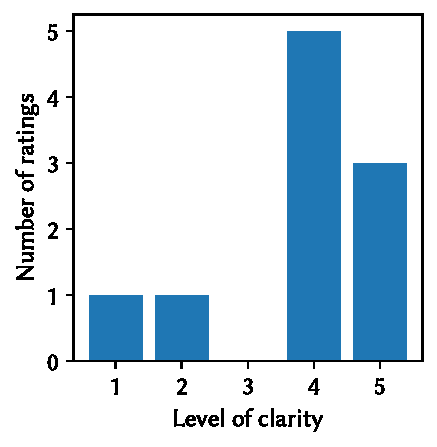
\includegraphics[width=0.48\textwidth]{img/pilot_survey_task_clearness.pdf}
%		\caption{Answers of the pilot survey participants to the question "How clear was your task?".}
		\label{fig:pilot-task-clear}
	\end{figure}
	
	\textbf{What problems were with the task? If there were none, leave blank.}
	\begin{itemize}
		\item Did at first not know where to rate the code.
		\item I was confused about the textfield for the comments because I only remembered that we should rate the code snippets, not that we have to make comments. Since I was not able to navigate back to the task description, I did not know what to do with them.
%		\item Für einen Anfänger mit sehr wenig Java Erfahrung ist meiner Meinung nach der Code zu kompliziert.
		\item Translated from German: In my opinion, the code is too complicated for a beginner with very little Java experience.
		\item In the first place, I didn't really understand what readability meant. But after slide 3 or 4, I understood what this was about.
		\item I found it difficult to categorize the first examples because you don't know what's still to come. For example, what the least readable code is.
	\end{itemize}

	\textbf{What problems were there with the survey tool? If there were none, leave blank.}
	\begin{itemize}
		\item Mobile is not easy to use because of the scrolling needed to complete the survey.
		\item First, I needed to figure out how this tool works and that the rating is done with the stars below. I thought I should write my rating as a comment in the comment field below. After number 20, I didn't know whether I could close the survey or not.
		\item I also thought that I should use the drop-down menu on the upper left.
		\item It is sometimes necessary to swipe horizontally to see all of the code, which is a bit inconvenient.
		\item Translated from German: In my opinion, the tool is not suitable for beginners. The code is too convoluted and sometimes incomprehensible.
		\item After finishing the task, at least a message should be shown.
		\item I didn't understand what the button at the top left meant, where you could select the programming language. There were too many fonts to choose. I also wasn't sure whether to write a comment or not. It wasn't described at the beginning.
	\end{itemize}

	\textbf{What improvements would you make to the survey? If none, leave blank.}
	\begin{itemize}
		\item Maybe one sentence that one should use the stars for the rating, then it would be clear. Also, the submit note after the last question could contain that one can close the survey now.
		\item I suggest making the task description accessible during the rating.
		\item Maybe the option to leave the survey when clicking to submit.
		\item Mehr Hilfestellung zum Lesen des Codes. Mehr Beschreibung oder ein zusätzliches Cheat Sheet mit Bedeutungen von Befehlen.
		\item I think it's a good idea to ask the participant at the beginning to explain what readability means for him.
		\item I would leave out the buttons described above. I was missing a scrollbar at the bottom of the code-window. A conclusion page with a message like "Thank you for your participation", "You're Done!" or other further information was missing, too.
	\end{itemize}
	
	\pagebreak
	
	\textbf{Do you have any other feedback? If none, leave blank.}
	\begin{itemize}
		\item There were drop downs for the programming language, but choosing another language did not change anything. It was a bit confusing that (almost?) all code snippets had very long imports within the code, which made them poorly readable.
		\item I spent the most time understanding methods with complete Java import names. (org.foo.bar.ClassName).
		\item GOOD LUCK
	\end{itemize}
	

\chapter{\RDMs Configuration File}\label{appendix:rdh-config-file}
	\begin{listing}[h!]
		\begin{minted}[linenos, frame=lines, framesep=2mm]{YAML}
			newline:
			- 0.0  # Probability for no newline
			- 1.0  # Probability for one newline
			incTab:
			- 0.0  # Probability for no tab
			- 1.0  # Probability for one tab
			decTab:
			- 0.0  # Probability for no tab
			- 1.0  # Probability for one tab
			space:
			- 0.0  # Probability for no space; Must be 0.0
			- 1.0  # Probability for one space
			newLineInsteadOfSpace: 0
			spaceInsteadOfNewline: 0
			incTabInsteadOfDecTab: 0
			decTabInsteadOfIncTab: 0
			renameVariable: 0
			renameField: 0
			renameMethod: 0
			inlineMethod: 0
			removeComment: 0
			add0: 0
			insertBraces: 0
			starImport: 0
			inlineField: 0
			partiallyEvaluate: 0
		\end{minted}
		\label{lst:rdh-config-file}
	\end{listing}
	

\chapter{Prolific Survey Texts}\label{appendix:prolific-survey-texts}
	\textbf{On Prolific:}
	
	Readability of Java Code
	
	We study the readability of Java source code. Therefore, please read Java methods and rate their readability on a scale from 1 (very unreadable) to 5 (very readable).
	
	\textbf{At the top of the tool:}
	
	Readability of Java Code
	
	Read the Java methods and rate their readability on a scale from 1 (very unreadable) to 5 (very readable) using the stars below the code box. To navigate between methods, use the arrows above or below the code box. Make sure to rate each snippet.
	
	\textbf{Introduction page 1:}
	
	This study aims to investigate the readability of Java source code. In this survey, we will show you 20 Java methods. Please read the methods thoroughly and rate how readable you think they are. Before we begin, please answer the following question:
	
	How would you describe your familiarity with Java?
	\begin{enumerate}
		\item Expert
		\item Advanced
		\item Intermediate
		\item Beginner
		\item Novice
	\end{enumerate}
	
	\pagebreak
	
	\textbf{Introduction Page 2:}
	
	Below is an example of the interface for displaying and rating the code. Use the stars below the code box for your rating. Please rate the readability on a scale from 1 (very unreadable) to 5 (very readable). At the top left, you can adjust the syntax highlighting and theme (dark/light) according to your preferences (optional). Comments are not available during this survey.
	
	[EXAMPLE]
	
	\textbf{Introduction Page 3:}
	
	This survey should take about 10 minutes to complete. Now you are ready to go! 


\chapter{Towards Model - Visual Encoding Colors}\label{appendix:model-visual-colors}	
	The following CSS was used to generate the background colors for the visual encoding. 
	You can find an overview over all tokens on the pygments homepage\curl{https://pygments.org/docs/tokens/}{2024-03-02}.

%	of the Towards model of \citeauthor{mi2022towards}~\cite{mi2022towards}

%/* Global Styles */
%* {
%	color: #fff;
%	background-color: #fff;
%	font-size: 2px;
%	padding: 0;
%	margin: 0;
%}

%	\begin{figure}[h!]
		\begin{minted}[linenos, frame=lines, framesep=2mm]{CSS}
			/* Comment Styles */
			.c, .ch, .cm, .cp, .cpf, .c1, .cs {
				background-color: #006200;
				color: #006200;
			}
			
			/* Keyword Styles */
			.k, .kc, .kd, .kn, .kp, .kr, .kt {
				background-color: #fa0200;
				color: #fa0200;
			}
			
			/* Parentheses, Semicolon, Braces Styles */
			.p, .o, .ow {
				background-color: #fefa01;
				color: #fefa01;
			}
			
			/* Whitespace Styles */
			.w {
				background-color: #fff;
				color: #fff;
			}
			
			
			/* Names/Identifiers Styles */
			.n, .na, .nb, .nc, .no, .nd, .ni, .ne, .nf, .nl, .nn, .nt, .nv {
				background-color: #01ffff;
				color: #01ffff;
			}
			
			/* Literals Styles */
			.m, .mb, .mf, .mh, .mi, .mo, .s, .sa, .sb, .sc, .dl, .sd, .s2, .se, .sh, .si, .sx, .sr, .s1, .ss, .b, .bp, .f, .fm, .v, .vc, .vg, .vi, .vm, .i, .il {
				background-color: #01ffff;
				color: #01ffff;
			}
			
			/* Error Styles */
			.err {
				background-color: #fff;
				color: #fff;
			}
			
			/* Generics Styles */
			.g, .gd, .ge, .ges, .gr, .gh, .gi, .go, .gp, .gs, .gu, .gt {
				background-color: #fefa01;
				color: #fefa01;
			}
		\end{minted}
		\label{lst:model-visual-css}
%	\end{figure}
	
\end{document}
